
%%
%% 
%% 
%%

\documentclass[letterpaper,10pt,conference]{ieeeconf}
\IEEEoverridecommandlockouts 

\newcommand{\stt}[1]{{\small\tt #1}} %\small\tt too small here
\newcommand{\powprof}{\stt{powprofiler}}
\newcommand{\figpath}{./figures}
\newcommand{\iu}{{i\mkern1mu}}
\let\labelindent\relax

\usepackage[inline]{enumitem}
\usepackage{booktabs}
\usepackage{flushend}
\usepackage{tikz}
\usetikzlibrary{automata,positioning,decorations.pathreplacing}
\usepackage[left=1in,right=1in,top=1in,bottom=1in]{geometry} 

%% citation packege
\usepackage{cite}

%% figures package
%\usepackage[pdftex]{graphicx}
%\graphicspath{{figures/}}
%\DeclareGraphicsExtensions{.pdf,.jpeg,.png}

%% math package
\usepackage{amsmath}
\usepackage{mathtools}
\usepackage{amssymb}
\usepackage{arydshln}
\DeclarePairedDelimiter{\ceil}{\lceil}{\rceil}

\let\proof\relax
\let\endproof\relax
\usepackage{amsthm}

%% pseudocode package
\usepackage{algpseudocode}

%% packages for alignment
%\usepackage{array}
%\usepackage{mdwmath}
%\usepackage{mdwtab}
%\usepackage{eqparbox}

%% packages for subfigures (eventually)
\usepackage[tight,footnotesize]{subfigure}
%\usepackage[caption=false]{caption}
%\usepackage[font=footnotesize]{subfig}
%\usepackage[caption=false,font=footnotesize]{subfig}

%% package for urls
\usepackage{url}

%% hyperref
% and an override to make hyperref work with ieeeconf.cls
\makeatletter
\let\NAT@parse\undefined
\makeatother
\usepackage{hyperref}

\usepackage{textpos}

\DeclarePairedDelimiter\abs{\lvert}{\rvert}%
\DeclarePairedDelimiter\norm{\lVert}{\rVert}%

%% correct bad hyphenation here
\hyphenation{}

\renewcommand{\qedsymbol}{$\blacksquare$}

\theoremstyle{definition}
\newtheorem{thm}{Theorem}[section]
\newtheorem{lem}[thm]{Lemma}
\newtheorem{prop}[thm]{Proposition}
\newtheorem{assm}[thm]{Assumption}
\newtheorem{cor}{Corollary}
\newtheorem{conj}{Conjecture}[section]
\newtheorem{defn}{Definition}[section]
\newtheorem{exmp}{Example}[section]
\newtheorem{rem}{Remark}

\DeclareMathOperator*{\argmax}{arg\,max}
\DeclareMathOperator*{\argmin}{arg\,min}

\algdef{SE}[DOWHILE]{Do}{doWhile}{\algorithmicdo}[1]{\algorithmicwhile\ #1}%

% just lines in pseudocode...
\usepackage{etoolbox}

\makeatletter
% start with some helper code
% This is the vertical rule that is inserted
\newcommand*{\algrule}[1][\algorithmicindent]{%
  \makebox[#1][l]{%
    \hspace*{.2em}% <------------- This is where the rule starts from
    \vrule height .75\baselineskip depth .25\baselineskip
  }
}

\newcount\ALG@printindent@tempcnta
\def\ALG@printindent{%
    \ifnum \theALG@nested>0% is there anything to print
    \ifx\ALG@text\ALG@x@notext% is this an end group without any text?
    % do nothing
    \else
    \unskip
    % draw a rule for each indent level
    \ALG@printindent@tempcnta=1
    \loop
    \algrule[\csname ALG@ind@\the\ALG@printindent@tempcnta\endcsname]%
    \advance \ALG@printindent@tempcnta 1
    \ifnum \ALG@printindent@tempcnta<\numexpr\theALG@nested+1\relax
    \repeat
    \fi
    \fi
}
% the following line injects our new indent handling code in place of the default spacing
\patchcmd{\ALG@doentity}{\noindent\hskip\ALG@tlm}{\ALG@printindent}{}{\errmessage{failed to patch}}
\patchcmd{\ALG@doentity}{\item[]\nointerlineskip}{}{}{} % no spurious vertical space
% end vertical rule patch for algorithmicx
\makeatother

% for blank page

\usepackage{afterpage}

%% references (generates a bib file for bibtex)
\begin{filecontents}{\jobname.bib}
  @inproceedings{seewald2020mechanical,
    title={Mechanical and Computational Energy Estimation of a Fixed-Wing Drone}, 
    author={Seewald, Adam and Garcia de Marina, Hector and Midtiby, Henrik Skov and Schultz, Ulrik Pagh},
    booktitle={2020 Fourth IEEE International Conference on Robotic Computing (IRC)},
    pages={135--142},
    year={2020},
    organization={IEEE},
    DOI={10.1109/IRC.2020.00028},
    url={https://adamseew.bitbucket.io/short/mechanical2020}
  }

  @article{seewald2019coarse,
    title={Coarse-Grained Computation-Oriented Energy Modeling for Heterogeneous Parallel Embedded Systems},
    author={Seewald, Adam and Schultz, Ulrik Pagh and Ebeid, Emad and Midtiby, Henrik Skov},
    journal={International Journal of Parallel Programming},
    pages={1--22},
    year={2019},
    publisher={Springer},
    DOI={10.1007/s10766-019-00645-y},
    url={https://adamseew.bitbucket.io/short/coarse2019}
  }
  @inproceedings{seewald2019component,
    title={Component-based computation-energy modeling for embedded systems},
    author={Seewald, Adam and Schultz, Ulrik Pagh and Roeder, Julius and Rouxel, Benjamin and Grelck, Clemens},
    booktitle={Proceedings Companion of the 2019 ACM SIGPLAN International Conference on Systems, Programming, Languages, and Applications: Software for Humanity},
    pages={5--6},
    year={2019},
    organization={ACM},
    DOI={10.1145/3359061.3362775},
    url={https://adamseew.bitbucket.io/short/component2019}
  }
  @inproceedings{hajjaj2014review,
    title={Review of research in the area of agriculture mobile robots},
    author={Hajjaj, Sami Salama Hussen and Sahari, Khairul Salleh Mohamed},
    booktitle={The 8th International Conference on Robotic, Vision, Signal Processing \& Power Applications},
    pages={107--117},
    year={2014},
    organization={Springer}
  }
  @inproceedings{qingchun2012study,
    title={Study on strawberry robotic harvesting system},
    author={Qingchun, Feng and Wengang, Zheng and Quan, Qiu and Kai, Jiang and Rui, Guo},
    booktitle={2012 IEEE International Conference on Computer Science and Automation Engineering (CSAE)},
    volume={1},
    pages={320--324},
    year={2012},
    organization={IEEE}
  }
  @article{edan2000robotic,
    title={Robotic melon harvesting},
    author={Edan, Yael and Rogozin, Dima and Flash, Tamar and Miles, Gaines E},
    journal={IEEE Transactions on Robotics and Automation},
    volume={16},
    number={6},
    pages={831--835},
    year={2000},
    publisher={IEEE}
  }
  @inproceedings{aljanobi2010setup,
    title={A setup of mobile robotic unit for fruit harvesting},
    author={Aljanobi, AA and Al-Hamed, SA and Al-Suhaibani, SA},
    booktitle={19th International Workshop on Robotics in Alpe-Adria-Danube Region (RAAD 2010)},
    pages={105--108},
    year={2010},
    organization={IEEE}
  }
  @article{de2011design,
    title={Design and control of an apple harvesting robot},
    author={De-An, Zhao and Jidong, Lv and Wei, Ji and Ying, Zhang and Yu, Chen},
    journal={Biosystems engineering},
    volume={110},
    number={2},
    pages={112--122},
    year={2011},
    publisher={Elsevier}
  }
  @article{dong2011development,
    title={Development of a row guidance system for an autonomous robot for white asparagus harvesting},
    author={Dong, Fuhong and Heinemann, Wolfgang and Kasper, Roland},
    journal={Computers and Electronics in Agriculture},
    volume={79},
    number={2},
    pages={216--225},
    year={2011},
    publisher={Elsevier}
  }
  @inproceedings{li2008analysis,
    title={Analysis of workspace and kinematics for a tomato harvesting robot},
    author={Li, Zhiguo and Liu, Jizhan and Li, Pingping and Li, Wei},
    booktitle={2008 International Conference on Intelligent Computation Technology and Automation (ICICTA)},
    volume={1},
    pages={823--827},
    year={2008},
    organization={IEEE}
  }
  @article{puri2017agriculture,
    title={Agriculture drones: A modern breakthrough in precision agriculture},
    author={Puri, Vikram and Nayyar, Anand and Raja, Linesh},
    journal={Journal of Statistics and Management Systems},
    volume={20},
    number={4},
    pages={507--518},
    year={2017},
    publisher={Taylor \& Francis}
  }
  @inproceedings{mei2005case,
    title={A case study of mobile robot's energy consumption and conservation techniques},
    author={Mei, Yongguo and Lu, Yung-Hsiang and Hu, Y Charlie and Lee, CS George},
    booktitle={ICAR'05. Proceedings., 12th International Conference on Advanced Robotics, 2005.},
    pages={492--497},
    year={2005},
    organization={IEEE}
  }
  @inproceedings{mei2004energy,
    title={Energy-efficient motion planning for mobile robots},
    author={Mei, Yongguo and Lu, Yung-Hsiang and Hu, Y Charlie and Lee, CS George},
    booktitle={IEEE International Conference on Robotics and Automation, 2004. Proceedings. ICRA'04. 2004},
    volume={5},
    pages={4344--4349},
    year={2004},
    organization={IEEE}
  }
  @article{mei2006deployment,
    title={Deployment of mobile robots with energy and timing constraints},
    author={Mei, Yongguo and Lu, Yung-Hsiang and Hu, Yu Charlie and Lee, CS George},
    journal={IEEE Transactions on robotics},
    volume={22},
    number={3},
    pages={507--522},
    year={2006},
    publisher={IEEE}
  }
  @inproceedings{kreciglowa2017energy,
    title={Energy efficiency of trajectory generation methods for stop-and-go aerial robot navigation},
    author={Kreciglowa, Nadia and Karydis, Konstantinos and Kumar, Vijay},
    booktitle={2017 International Conference on Unmanned Aircraft Systems (ICUAS)},
    pages={656--662},
    year={2017},
    organization={IEEE}
  }
  @article{sadrpour2013mission,
    title={Mission Energy Prediction for Unmanned Ground Vehicles Using Real-time Measurements and Prior Knowledge},
    author={Sadrpour, Amir and Jin, Jionghua and Ulsoy, A Galip},
    journal={Journal of Field Robotics},
    volume={30},
    number={3},
    pages={399--414},
    year={2013},
    publisher={Wiley Online Library}
  }
  @inproceedings{sadrpour2013experimental,
    title={Experimental validation of mission energy prediction model for unmanned ground vehicles},
    author={Sadrpour, Amir and Jin, Judy and Ulsoy, A Galip},
    booktitle={2013 American Control Conference},
    pages={5960--5965},
    year={2013},
    organization={IEEE}
  }
  @inproceedings{kim2005energy,
    title={Energy-saving 3-step velocity control algorithm for battery-powered wheeled mobile robots},
    author={Kim, Chong Hui and Kim, Byung Kook},
    booktitle={Proceedings of the 2005 IEEE international conference on robotics and automation},
    pages={2375--2380},
    year={2005},
    organization={IEEE}
  }
  @inproceedings{kim2008minimum,
    title={Minimum-energy translational trajectory planning for battery-powered three-wheeled omni-directional mobile robots},
    author={Kim, Hongjun and Kim, Byung-Kook},
    booktitle={2008 10th International Conference on Control, Automation, Robotics and Vision},
    pages={1730--1735},
    year={2008},
    organization={IEEE}
  }
  @book{wahab2015energy,
    title={Energy modeling of differential drive robots},
    author={Wahab, Mudasser and Rios-Gutierrez, Fernando and El Shahat, Adel},
    year={2015},
    publisher={IEEE}
  }
  @online{px4,
    author={PX4},
    title={{PX4} open-source autopilot},
    url={https://px4.io/},
    urldate={2016-09-01}
  }
  @online{papa,
    author={Paparazzi},
    title={{UAV} open-source project},
    url={http://wiki.paparazziuav.org/},
    urldate={2016-09-01}
  }
  @online{nano,
    author={NVIDIA},
    title={{NVIDIA Jetson Nano} developer kit},
    url={https://developer.nvidia.com/embedded/jetson-nano-developer-kit},
    urldate={2020-02-02}
  }
  @online{opterra,
    author={Horizon Hobby},
    title={{Opterra} 2m Wing BNF Basic},
    url={https://www.horizonhobby.com/opterra-2m-wing-bnf-basic-p-efl11150},
    urldate={2020-02-02}
  }
  @online{meier2013mavlink,
    title={Mavlink: Micro air vehicle communication protocol},
    author={Meier, Lorenz and Camacho, J and Godbolt, B and Goppert, J and Heng, L and Lizarraga, M and others},
    url={https://mavlink.io/},
    urldate={2020-02-02}
  }
  @article{ullah2018pednet,
    title={Pednet: A spatio-temporal deep convolutional neural network for pedestrian segmentation},
    author={Ullah, Mohib and Mohammed, Ahmed and Alaya Cheikh, Faouzi},
    journal={Journal of Imaging},
    volume={4},
    number={9},
    pages={107},
    year={2018},
    publisher={Multidisciplinary Digital Publishing Institute}
  }
  @inproceedings{sandler2018mobilenetv2,
    title={Mobilenetv2: Inverted residuals and linear bottlenecks},
    author={Sandler, Mark and Howard, Andrew and Zhu, Menglong and Zhmoginov, Andrey and Chen, Liang-Chieh},
    booktitle={Proceedings of the IEEE conference on computer vision and pattern recognition},
    pages={4510--4520},
    year={2018}
  }
  @inproceedings{quigley2009ros,
    title={ROS: an open-source Robot Operating System},
    author={Quigley, Morgan and Conley, Ken and Gerkey, Brian and Faust, Josh and Foote, Tully and Leibs, Jeremy and Wheeler, Rob and Ng, Andrew Y},
    booktitle={ICRA workshop on open source software},
    volume={3},
    number={3.2},
    pages={5},
    year={2009}
  }
  @book{stengel1994optimal,
    title={Optimal control and estimation},
    author={Stengel, Robert F},
    year={1994},
    publisher={Courier Corporation}
  }
  @book{simon2006optimal,
    title={Optimal state estimation: Kalman, H infinity, and nonlinear approaches},
    author={Simon, Dan},
    year={2006},
    publisher={John Wiley \& Sons}
  }
  @inproceedings{de2017guidance,
    title={Guidance algorithm for smooth trajectory tracking of a fixed wing UAV flying in wind flows},
    author={De Marina, Hector Garcia and Kapitanyuk, Yuri A and Bronz, Murat and Hattenberger, Gautier and Cao, Ming},
    booktitle={2017 IEEE international conference on robotics and automation (ICRA)},
    pages={5740--5745},
    year={2017},
    organization={IEEE}
  }
  @book{rawlings2017model,
    title={Model predictive control: theory, computation, and design},
    author={Rawlings, James Blake and Mayne, David Q and Diehl, Moritz},
    volume={2},
    year={2017},
    publisher={Nob Hill Publishing Madison, WI}
  }
  @inproceedings{morbidi2016minimum,
    title={Minimum-energy path generation for a quadrotor UAV},
    author={Morbidi, Fabio and Cano, Roel and Lara, David},
    booktitle={2016 IEEE International Conference on Robotics and Automation (ICRA)},
    pages={1492--1498},
    year={2016},
    organization={IEEE}
  }
  @inproceedings{daponte2019review,
    title={A review on the use of drones for precision agriculture},
    author={Daponte, Pasquale and De Vito, Luca and Glielmo, Luigi and Iannelli, Luigi and Liuzza, Davide and Picariello, Francesco and Silano, Giuseppe},
    booktitle={IOP Conference Series: Earth and Environmental Science},
    volume={275},
    number={1},
    pages={012022},
    year={2019},
    organization={IOP Publishing}
  }
  @inproceedings{zamanakos2020energy,
    title={Energy-Aware Design of Vision-Based Autonomous Tracking and Landing of a UAV}, 
    author={Zamanakos, Georgios and Seewald, Adam and Midtiby, Henrik Skov and Schultz, Ulrik Pagh},
    booktitle={2020 Fourth IEEE International Conference on Robotic Computing (IRC)},
    pages={294--297},
    year={2020},
    organization={IEEE},
    DOI={10.1109/IRC.2020.00054},
    url={https://adamseew.bitbucket.io/short/energy2020}
  }

  @inproceedings{seewald2020beyond,
    title={Beyond Traditional Energy Planning: the Weight of Computations in Planetary Exploration}, 
    author={Seewald, Adam},
    booktitle={IROS Workshop on Planetary Exploration Robots: Challenges and Opportunities (PLANROBO20)},
    pages={3},
    year={2020},
    publisher={ETH Zurich, Department of Mechanical and Process Engineering},
    DOI={10.3929/ethz-b-000450120},
    url={https://adamseew.bitbucket.io/short/beyond2020}
  }
  @inproceedings{lindemann2005smoothly,
    title={Smoothly blending vector fields for global robot navigation},
    author={Lindemann, Stephen R and LaValle, Steven M},
    booktitle={Proceedings of the 44th IEEE Conference on Decision and Control},
    pages={3553--3559},
    year={2005},
    organization={IEEE}
  }
  @article{gonccalves2010vector,
    title={Vector fields for robot navigation along time-varying curves in $n$-dimensions},
    author={Gon{\c{c}}alves, Vin{\'\i}cius M and Pimenta, Luciano CA and Maia, Carlos A and Dutra, Bruno CO and Pereira, Guilherme AS},
    journal={IEEE Transactions on Robotics},
    volume={26},
    number={4},
    pages={647--659},
    year={2010},
    publisher={IEEE}
  }
  @inproceedings{panagou2014motion,
    title={Motion planning and collision avoidance using navigation vector fields},
    author={Panagou, Dimitra},
    booktitle={2014 IEEE International Conference on Robotics and Automation (ICRA)},
    pages={2513--2518},
    year={2014},
    organization={IEEE}
  }
  @inproceedings{zhou2014vector,
    title={Vector field following for quadrotors using differential flatness},
    author={Zhou, Dingjiang and Schwager, Mac},
    booktitle={2014 IEEE International Conference on Robotics and Automation (ICRA)},
    pages={6567--6572},
    year={2014},
    organization={IEEE}
  }
  @article{kapitanyuk2017guiding,
    title={A guiding vector-field algorithm for path-following control of nonholonomic mobile robots},
    author={Kapitanyuk, Yuri A and Proskurnikov, Anton V and Cao, Ming},
    journal={IEEE Transactions on Control Systems Technology},
    volume={26},
    number={4},
    pages={1372--1385},
    year={2017},
    publisher={IEEE}
  }
  @book{kuo1967automatic,
    title={Automatic Control Systems},
    author={Kuo, B.C.},
    isbn={9780130549730},
    lccn={67016388},
    series={Electrical engineering series},
    year={1967},
    publisher={Prentice-Hall}
  }
  @article{moler2003nineteen,
    title={Nineteen dubious ways to compute the exponential of a matrix, twenty-five years later},
    author={Moler, Cleve and Van Loan, Charles},
    journal={SIAM review},
    volume={45},
    number={1},
    pages={3--49},
    year={2003},
    publisher={SIAM}
  }
  @book{ogata2002modern,
    title={Modern Control Engineering},
    author={Ogata, K.},
    isbn={9780130432452},
    lccn={2001021683},
    year={2002},
    publisher={Prentice Hall}
  }
  @article{rizvi2017general,
    title={A general-purpose graphics processing unit (gpgpu)-accelerated robotic controller using a low power mobile platform},
    author={Rizvi, Syed Tahir Hussain and Cabodi, Gianpiero and Patti, Denis and Gulzar, Muhammad Majid},
    journal={Journal of Low Power Electronics and Applications},
    volume={7},
    number={2},
    pages={10},
    year={2017},
    publisher={Multidisciplinary Digital Publishing Institute}
  }
  @article{abramov2012real,
    title={Real-time segmentation of stereo videos on a portable system with a mobile gpu},
    author={Abramov, Alexey and Pauwels, Karl and Papon, Jeremie and Worgotter, Florentin and Dellen, Babette},
    journal={IEEE Transactions on Circuits and Systems for Video Technology},
    volume={22},
    number={9},
    pages={1292--1305},
    year={2012},
    publisher={IEEE}
  }
  @inproceedings{jaramillo2019visual,
    title={Visual saliency with foveated images for fast object detection and recognition in mobile robots using low-power embedded GPUs},
    author={Jaramillo-Avila, Uziel and Aitken, Jonathan M and Anderson, Sean R},
    booktitle={2019 19th International Conference on Advanced Robotics (ICAR)},
    pages={773--778},
    year={2019},
    organization={IEEE}
  }
  @inproceedings{satria2016real,
    title={Real-time system-level implementation of a telepresence robot using an embedded GPU platform},
    author={Satria, Muhammad Teguh and Gurumani, Swathi and Zheng, Wang and Tee, Keng Peng and Koh, Augustine and Yu, Pan and Rupnow, Kyle and Chen, Deming},
    booktitle={2016 Design, Automation \& Test in Europe Conference \& Exhibition (DATE)},
    pages={1445--1448},
    year={2016},
    organization={IEEE}
  }

\end{filecontents}

\title{\LARGE \bf
Energy-Aware Dynamic Planning Algorithm for Autonomous UAVs
}

%% author names and affiliations
\author{
  Adam Seewald$^{1}$, Hector Garcia de Marina$^{2}$, and Ulrik Pagh Schultz$^{1}$
  \thanks{This work is supported and partly funded by the European Union's Horizon2020 research and innovation program under grant agreement No. 779882 (TeamPlay).
  }
  \thanks{$^{1}$Adam Seewald, Ulrik Pagh Schultz are with the SDU UAS Center, M{\ae}rsk Mc-Kinney M{\o}ller Institute, University of Southern Denmark, Odense, Denmark. Email: {\tt\small ads@mmmi.sdu.dk}.}
  \thanks{$^{2}$Hector Garcia de Marina is with the Faculty of Physics, Department of Computer Architecture and Automatic Control, Universidad Computense de Madrid, Spain.}
}

\begin{document}

%% make the title area
\maketitle

\thispagestyle{empty}
\pagestyle{empty}

\begin{abstract}

  abstract\\
  abstract\\
  abstract\\
  abstract\\
  abstract\\
  abstract\\
  abstract\\
  abstract\\
  abstract\\
  abstract\\
  abstract\\
  abstract\\
  abstract\\
  abstract
\end{abstract}

% For peer review papers, you can put extra information on the cover
% page as needed:
% \ifCLASSOPTIONpeerreview
% \begin{center} \bfseries EDICS Category: 3-BBND \end{center}
% \fi
%
% For peerreview papers, this IEEEtran command inserts a page break and
% creates the second title. It will be ignored for other modes.
\IEEEpeerreviewmaketitle


%%%%%%%%%%%%%%%%%%%%%%
\section{Introduction}
\label{sec:intro}

Many scenarios involving unmanned aerial vehicles (UAVs), such as precision agriculture, search and rescue, and surveillance, require high autonomy but have limited energy budgets. A typical example of these scenarios is a UAV flying a path and performing some on-board computational tasks. For instance, the UAV might detect ground patterns and inform other ground-based actors with little human interaction. We refer to the computational tasks that can be dynamically replanned as computations. We are interested in energy-aware dynamic planning, which would find optimal tradeoffs between the path, computations, and energy requirements. Current generic planning solutions for outdoor UAVs do not plan path and computations dynamically, nor are energy-aware. They are often semi-autonomous; the plan--the path and computations--is static and usually defined using planning software~\cite{daponte2019review}. Such a state of practice has prompted us to propose an \emph{energy-aware dynamic planning algorithm} for UAVs. The algorithm combines and generalizes some of the past body of knowledge on mobile robot planning problems and addresses the increasing \emph{computational demands} and their relation to energy consumption, path, and autonomy for the UAV planning problem.

Planning algorithms literature for mobile robots includes topics such as trajectory generation and path planning. Generally, the algorithms select an energy-optimized trajectory~\cite{mei2004energy}, e.g., by maximizing the operational time~\cite{wahab2015energy}. However, they apply to a small number of robots~\cite{kim2005energy}, and focus exclusively on planning the trajectory for these robots~\cite{kim2008minimum}, despite compelling evidence for the energy consumption also being significantly influenced by computations~\cite{mei2005case}. Given the availability of powerful GPU-equipped mobile hardware~\cite{rizvi2017general}, the use of computations is expected to increase in the near future~\cite{abramov2012real,satria2016real,jaramillo2019visual}. More complex planning, which includes a broader concept of the plan being a set of tasks and a path, all focus on the trajectory~\cite{mei2005case,mei2006deployment} and apply to a small number of robots~\cite{sadrpour2013mission,sadrpour2013experimental}. For UAVs specifically, rotorcrafts have gained interest in terms of algorithms for energy-optimized trajectory generation~\cite{morbidi2016minimum,kreciglowa2017energy}. 

Unlike most of the past planning algorithms literature, our algorithm plans both the path and computations. We guide the UAV using a vector field~\cite{de2017guidance} that converges smoothly to a planned trajectory. The use of vector fields for planning is widely discussed in the literature~\cite{lindemann2005smoothly,gonccalves2010vector,panagou2014motion,zhou2014vector,kapitanyuk2017guiding,de2017guidance}. We denote the trajectory with a mathematical function that we refer to as the trajectory explicit equation (TEE). The path is composed of multiple TEEs. We express the computations with a modeling tool presented in our previous work~\cite{seewald2019coarse}. The algorithm alters the TEE and computations within some parameters using output model predictive control (MPC). These parameters are the maximum, minimum, and current levels of the TEE and computations. The user specifies the parameters in an initial plan with an energy budget. The energy budget is the battery capacity and some other battery parameters. In the remainder of the paper, we adopt the following notation. We refer to the current TEE and computations parameters simply as TEE and computations parameters. We refer to both as parameters. We refer to the constraints sets that delimit the maximum and minimum levels of the parameters as TEE set and computations sets, and to both as parameters sets. There can be multiple or none computations parameters per each task, and the same applies to the TEE. There is one TEE set but multiple computations sets, one per each computation parameter. Our goal is to complete the plan with the highest possible parameters as the UAV flies and its batteries drain. The term parameters should not be confused with the battery parameters, which we always mention explicitly. These are fixed values that are not replanned by the algorithm.

To achieve the energy-aware dynamic planning, we further introduce and formally proof a periodic energy model that accounts for the uncertainty (atmospheric interference). We use Fourier analysis to derive the model, and state estimation to address the uncertainty. Periodicity is often present due to the path and computations repetitive patterns~\cite{seewald2020mechanical}. Indeed UAV scenarios often iterate over a set of tasks and trajectories (e.g., monitoring or search and rescue). Given that the plan is periodic, we expect the energy to approximately evolve periodically. 
The observation applies broadly; we show different UAV scenarios with periodic energy signals. Moreover, we briefly investigate such signals in some ground-based mobile robots.

In the spirit of reducing costs and resources, we showcase the algorithm using the problem of dynamic planning for a precision agriculture fixed-wing UAV. Precision agriculture is often put into practice~\cite{hajjaj2014review} with ground mobile robots used for harvesting~\cite{qingchun2012study,dong2011development, de2011design, aljanobi2010setup, li2008analysis, edan2000robotic}, and UAVs for preventing damage and ensuring better crop quality~\cite{puri2017agriculture, daponte2019review}. The plan is structured as follows. Trajectory-wise, the UAV flies in circles and lines covering a polygon. Computationally-wise, it detects obstacles using a convolutional neural network (CNN) and informs grounded mobile robots employed for harvesting. The algorithm alters the plan; it controls the processing rate and the radius of the circles (affecting the distance between the lines). Figure~\ref{fig:overview} shows an initial slice of such a plan. The UAV first heads to a circular TEE with a given radius, which is later reduced as, e.g., windy weather requires the adjustment of the control input to avoid battery depletion. Computations significantly impact the battery, with a potential extension of up to 13 minutes over an hour by merely switching to the lowest computations (see Section~\ref{sec:experimental}).

The remainder of the paper is organized as follows. The overview of dynamic planning is provided in Section~\ref{sec:prob}, along with a suitable model for the position and energy. The algorithm is proposed in Section~\ref{sec:algo}. Section~\ref{sec:experimental} presents the result and showcases the performances. We propose some conclusions in Section~\ref{sec:conclusion}. Finally, we provide some additional information and examples in Appendixes~\ref{app:proof-eqv}--\ref{app:simulator}.


%%%%%%%%%%%%%%%%%%%%%%%%%%%%%%%%%%%
\section{Planning Overview}
\label{sec:prob}

The algorithm takes as input a user-specified initial plan that consists of different stages and some initial guesses that are necessary for the position and energy estimation. At each stage, the UAV must follow the TEE within TEE set and do the computations within the computations sets. The algorithm outputs the new position, the instantaneous energy consumption, and the control.

Let us assume the TEE at stage $i$ can be altered with $\rho$ TEE parameters and the computations with $\sigma$ computations parameters. We then express the TEE as a continuous twice differentiable function $\varphi_i:\mathbb{R}^2\times\mathbb{R}^\rho\rightarrow\mathbb{R}$ of a point and the TEE parameters. The TEE returns a metric of the distance between the point and the nominal trajectory. We express the computations as the value of the computations parameters. We discuss the concrete meaning of the value of TEE parameters in Subsection~\ref{sec:model}, and of the computations parameters in Subsection~\ref{sec:computations-model}. 

Let us adopt the following mathematical notation. Given an integer $a$, $[a]$ is the set $\{0,1,\dots,a\}$, $[a]^+$ the set $[a]/\{0\}$. $c_{i,j}$ specifues the $j$-th parameter of the $i$-th parameters set $c_i$. $c_{i,j}^0$ is the optimal value of the parameter $c_{i,j}$, and $\underline{c}_{i,j},\overline{c}_{i,j}$ its lower and upper bounds. We store these bounds in the plan specification, which format we discuss in Subsection~\ref{sec:plan}. The set $\langle c_{i,1},c_{i,2},...,c_{i,n}\rangle$ is an ordered list of $n$ parameters.

\begin{defn}[Stage, plan, and triggering point]\label{def:mission}
  A \emph{stage} $\Gamma_i$ at time instant $k$ of a plan $\Gamma$ is defined as the ordered list
  \begin{equation}\label{eq:mission}\begin{split}
    \Gamma_i:=\{\langle&\varphi_i(\mathbf{p}_k,c_{i,1},\dots,c_{i,\rho}),c_{i,\rho+1},\dots,c_{i,\rho+\sigma}\rangle\\\mid
    &\,\exists\,\,\mathbf{p}_k,\,\varphi_i(\mathbf{p}_k,c_{i,1},\dots,c_{i,\rho})\in\mathbb{C}_i,\,\\
      &\,\forall j\in[\sigma]^+,\,c_{i,\rho+j}\in\mathbb{S}_{i,j}\,\},
  \end{split}\end{equation}
  where $\mathbb{C}_i:=[\underline{c}_i,\overline{c}_i]\subseteq\mathbb{R}$ is the TEE set, and $\mathbb{S}_{i,j}:=[\underline{c}_{i,\rho+j},\overline{c}_{i,\rho+j}]\subseteq\mathbb{Z}_{\geq 0}$ the $j$-th computation set. $\mathbf{p}_k$ is a point of a UAV flying at an assigned altitude $h\in\mathbb{R}_{>0}$ w.r.t. some inertial navigation frame $\mathcal{O}_W$.

  The \emph{plan} is a finite state machine $\Gamma$ where the state-transition function $\bigcup_i{\Gamma_i}\times\mathbb{R}^2\rightarrow\bigcup_i{\Gamma_i}$ maps a stage and a point to the next stage. The point $\mathbf{p}_{\Gamma_{i}}$ that allows the transition between $\Gamma_i$ and $\Gamma_{i+1}$ is called \emph{triggering point}.
\end{defn}

\begin{figure}[h]
  \center
  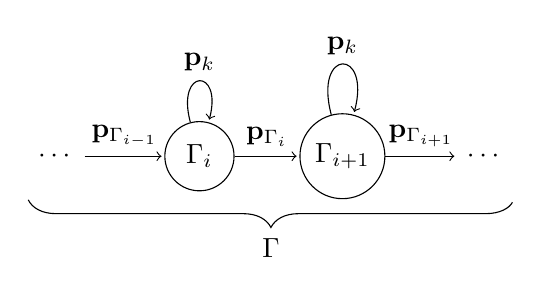
\begin{tikzpicture}[shorten >=1pt,node distance=12ex,on grid,auto] 
    \node        (q_dots0) {$\cdots$};
    \node[state] (q_0) [right=of q_dots0] {$\Gamma_i$};
    \node[state] (q_1) [right=of q_0] {$\Gamma_{i+1}$};
    \node        (q_dots1) [right=of q_1] {$\cdots$};   
    \path[->]
    (q_dots0) edge node{$\mathbf{p}_{\Gamma_{i-1}}$} (q_0)
    (q_0) edge node {$\mathbf{p}_{\Gamma_i}$} (q_1)    
    (q_0) edge [loop above] node {$\mathbf{p}_{k}$} (q_0)
    (q_1) edge node {$\mathbf{p}_{\Gamma_{i+1}}$} (q_dots1)
    (q_1) edge [loop above] node {$\mathbf{p}_{k}$} (q_1)
    ; %end path 
    \draw [decorate,decoration={brace,amplitude=10pt,mirror,raise=10pt},yshift=0pt]
    (q_dots0.south west) -- (q_dots1.south east) node [black,midway,yshift=-8ex]{$\Gamma$};
  \end{tikzpicture}
  \caption{The plan defined as a finite state machine}
  \label{fig:state-machine}
\end{figure}

A slice of the plan in Figure~\ref{fig:state-machine} shows the transition between the stages. The triggering point $\mathbf{p}_{\Gamma_{i-1}}$ allows the transition to stage $\Gamma_i$. The UAV remains in the stage with any generic point $\mathbf{p}_k$. It eventually enters the stage $\Gamma_{i+1}$ with the triggerint point $\mathbf{p}_{\Gamma_i}$ and so on, until it reaches the last triggering point.

\subsection{Plan specification file format}
\label{sec:plan}

The algorithm reads the plan $\Gamma$ from a file--the plan specification--with a specific file format. We refer the reader to Appendix~\ref{app:plan-example} for an example.

The first stage $\Gamma_1$ is expressed in the first line of the file
\begin{algorithmic}[1]
  \State\textbf{\texttt{$k_e$;$r$;$\varphi_1(\mathbf{p}_k,c_{1,1},\dots,c_{1,\rho})$}}\label{code:stage}
\end{algorithmic}
where $k_e$ is a convergence value, $r$ a rotation, and $\varphi_1$ the TEE. In the next subsection where we discuss the physical meaning of the convergence value and rotation. The rotation is expressed in binary format with zero being the counter-clockwise rotation, one the clockwise rotation.

The next line specifies the triggering point $\mathbf{p}_{\Gamma_1}$
\begin{algorithmic}[1]
  \setcounterref{ALG@line}{code:stage}
  \State\textbf{\texttt{$x$,$y$}}\label{code:trigger-pt}
\end{algorithmic}
where $x$ and $y$ are the two coordinates of the point. The UAV reaches the point within a given radius (a parameter of the algorithm) and enters the next stage $\Gamma_2$. The coordinates can be expressed in function of the TEE parameters $c_{1,1},\dots,c_{1,\rho}$. Generally, one can express the coordinates in function of the $i$-th TEE parameters $c_{i,1},\dots,c_{i,\rho}$, or any previous TEE parameters, propagating the information therein if necessary. See Figure~\ref{fig:state-machine2} where, for simplicity, we neglected the $\sigma=0$ computations parameters $c_i=c_{i,1},\dots,c_{i,\rho}$.

\begin{figure}[h]
  \center
  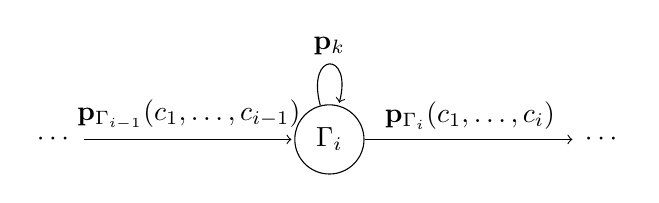
\begin{tikzpicture}[shorten >=1pt,node distance=23ex,on grid,auto] 
    \node        (q_dots0) {$\cdots$};
    \node[state] (q_0) [right=of q_dots0] {$\Gamma_i$};
    \node        (q_dots1) [right=of q_0] {$\cdots$};   
    \path[->]
    (q_dots0) edge node{$\mathbf{p}_{\Gamma_{i-1}}(c_1,\dots,c_{i-1})$} (q_0)
    (q_0) edge node {$\mathbf{p}_{\Gamma_i}(c_1,\dots,c_{i})$} (q_dots1)    
    (q_0) edge [loop above] node {$\mathbf{p}_{k}$} (q_0)
    ; %end path
  \end{tikzpicture}
  \caption{Detail of the stage $\Gamma_i$ in the finite state machine}
  \label{fig:state-machine2}
  \end{figure}

We refer the reader again to the example in Appendix~\ref{app:plan-example} for a detailed implementation. In the example, the first TEE parameter is propagated to all the following TEEs and triggering points. 

The line
\begin{algorithmic}[1]
  \setcounterref{ALG@line}{code:trigger-pt}
  \State\textbf{\texttt{[$\underline{c}_1$,$\overline{c}_1$]}}\label{code:tee-set}
\end{algorithmic}
specifies the lower $\underline{c}_{1}$ and upper $\overline{c}_{1}$ bounds of the TEE $\varphi_1$.

The following $\sigma$ lines
\begin{algorithmic}[1]
  \setcounterref{ALG@line}{code:tee-set}
  \State\textbf{\texttt{[$\underline{c}_{1,j}$,$\overline{c}_{1,j}$]}}\label{code:parameter-set}
\end{algorithmic}
specifies the lower $\underline{c}_{1,j}$ and upper $\overline{c}_{1,j}$ bounds of the $j$-th computation parameter set. They are in ascending order. 

This means that for the first stage, the algorithm can alter the TEE satisfying $\varphi_1\in\mathbb{C}_1$, and it can alter the computations individually. In fact the $j$-th computation parameter has to be in $\mathbb{S}_{1,j}$.

Follows the entries for stage $\Gamma_2$ (equivalent to lines~\ref{code:stage}--\ref{code:parameter-set}), $\Gamma_3$ and so on, until the last stage. We assume that the last triggering point is the final UAV position.

\subsection{State: position $\mathbf{p}$}
\label{sec:model}

We model the position with $(x,y)\in\mathbf{p}$ coordinates and the altitude $h$, and derive its evolution using vector field~\cite{de2017guidance}.

Let us assume that the set
\begin{equation}\label{eq:area}
  \mathcal{P}_i:=\{\mathbf{p}_k\mid\varphi_i(\mathbf{p}_k,c_{i,1},\dots,c_{i,\rho})\in\mathbb{C}_i\},
\end{equation}
delimits the area where the $i$-th TEE $\varphi_i$ is free to evolve using the TEE parameters $c_{i,1},...,c_{i,\rho}$ (the gray area in Figure~\ref{fig:overview}). $\varphi_i$ is a function of the two coordinates and is equal to zero when a point $\mathbf{p}_k$ is on the TEE. Physically, this means the UAV is flying exactly over the nominal trajectory. The TEE parameters allows to change the TEE. They are a way to alter the nominal trajectory in the initial plan.
In fact, the algorithm uses the set from Equation~(\ref{eq:area}) to alter the optimal TEE parameters $c_i^0$ (here we again neglect for simplicity the $\sigma=0$ computations parameters), such that $\varphi_i(\mathbf{p}_k,c_i^0)$ has the highest instantaneous energy consumption (while still respecting the energy budget). 

We derive the new position $\mathbf{p}_{k+1}$ using the function $\varPhi:=\varphi_i(\mathbf{p}_k,\mathbf{c}_i^0)$, computing its vector field $\nabla\varPhi:=\begin{bmatrix}\partial\varPhi/\partial x & \partial\varPhi/\partial y\end{bmatrix}^T$, and the direction to follow in the form of velocity vector
\begin{equation}\label{eq:pd}
  \dot{\mathbf{p}}_d(\mathbf{p}_k):=E\nabla\varPhi-k_e\varPhi\nabla\varPhi,\,\,\,E=\begin{bmatrix}
    0&1\\-1&0
  \end{bmatrix},
\end{equation}
where $E$ specifies the rotation (which influence the tracking direction), and $k_e\in\mathbb{R}_{\geq 0}$ the gain to adjusts the speed of convergence. The direction the velocity vector $\dot{\mathbf{p}}_d$ is pointing at is generally different from the course heading due to the atmospheric interference, such as wind ($w\in\mathbb{R}$ in Figure~\ref{fig:overview}).

\begin{figure}[h]
  \centering
  
\definecolor{cDEDEDE}{RGB}{222,222,222}
\definecolor{c2B2B2B}{RGB}{43,43,43}
\definecolor{cFFFFFF}{RGB}{255,255,255}
\definecolor{c9B9B9B}{RGB}{155,155,155}
\definecolor{c989898}{RGB}{152,152,152}
\definecolor{c4D4D4D}{RGB}{77,77,77}


\def \globalscale {.870000}
\begin{tikzpicture}[y=0.80pt, x=0.80pt, yscale=-\globalscale, xscale=\globalscale, inner sep=0pt, outer sep=0pt]
\path[fill=cDEDEDE,line join=round,line width=1.280pt] (11.6098,143.2690) -- (11.6381,143.2690) .. controls (12.6918,105.8790) and (43.0061,75.8094) .. (80.4938,75.1490) -- (80.4938,111.5790) .. controls (63.0922,112.2190) and (49.0572,126.0420) .. (48.0821,143.3560) -- (48.0967,157.7040) -- (48.0821,158.0290) -- (48.0821,158.3590) .. controls (48.0975,159.1860) and (48.2166,160.0470) .. (48.1937,160.8610) -- (48.1998,160.8690) -- (48.1998,162.8820) -- (48.0821,208.4660) -- (48.0821,216.6680) -- (48.0610,216.6680) -- (48.0605,216.8310) -- (48.0484,217.7520) -- (48.1143,221.9450) -- (11.4101,221.9530) .. controls (11.4101,220.0520) and (11.3860,223.8120) .. (11.3745,219.6040) -- (11.3745,217.8520) -- (11.3745,217.4970) -- (11.3745,217.0210) -- (11.3745,216.6730) -- (11.3745,145.5000) -- (11.6098,143.2690) -- cycle;



\path[draw=c2B2B2B,line join=round,line width=0.512pt] (81.7300,145.1480) ellipse (1.9796cm and 1.9796cm);



\path[draw=black,line join=round,line width=0.512pt] (84.1885,147.4600) -- (79.3297,142.5950);



\path[draw=black,line join=round,line width=0.512pt] (79.3321,147.4590) -- (84.1972,142.5950);



\path[draw=c2B2B2B,line join=round,line width=0.512pt] (11.6130,57.9496) -- (11.6123,221.7820);



\path[draw=black,line join=round,line width=0.512pt] (81.8116,145.0640) -- (11.5289,145.0640);



\path[fill=black,line join=round,line width=0.256pt] (17.2158,147.6960) -- (17.2088,142.3370) -- (12.3038,145.0230) -- (17.2158,147.6960) -- cycle;



\path[draw=black,line join=round,line width=1.024pt] (86.9347,19.9572) .. controls (95.0742,22.1535) and (96.9997,30.5095) .. (96.9997,30.5095) .. controls (96.9997,30.5095) and (112.2540,68.0133) .. (71.9151,75.7553) .. controls (66.6769,76.7607) and (67.8409,77.7130) .. (70.6628,77.6073);



\path[draw=black,fill=cFFFFFF,line join=round,line width=0.512pt] (103.4020,39.3713) -- (99.4578,23.0489) -- (95.8475,27.2484) -- (90.3755,28.7747) -- (103.4020,39.3713) -- cycle;



  \path[fill=cFFFFFF,line join=round,line width=1.024pt,rounded corners=0.0000cm] (4.7286,68.9128) rectangle (18.8758,87.0599);



  \path[cm={{1.0,0.0,0.0,1.0,(3.0,83.0)}}] (0.0000,0.0000) node[above right] () {$\varphi_2$};



  \path[fill=cFFFFFF,line join=round,line width=1.024pt,rounded corners=0.0000cm] (100.3810,72.5529) rectangle (118.5282,86.7001);



  \path[cm={{1.0,0.0,0.0,1.0,(102.0,86.0)}}] (0.0000,0.0000) node[above right] () {$\varphi_1$};



  \path[fill=cFFFFFF,line join=round,line width=1.024pt] (55.4211,215.8850) -- (41.2739,215.8850) -- (41.2532,229.5530) -- (55.4334,229.5530) -- (55.4211,215.8850) -- cycle;



  \path[cm={{1.0,0.0,0.0,1.0,(44.0,228.0)}}] (0.0000,0.0000) node[above right] () {$\underline{c}_1$};



  \path[fill=cFFFFFF,line join=round,line width=1.024pt] (69.0222,142.0810) -- (48.8751,142.0800) -- (48.8751,156.2270) -- (69.0222,156.2280) -- (69.0222,142.0810) -- cycle;



  \path[cm={{1.0,0.0,0.0,1.0,(50.0,156.0)}}] (0.0000,0.0000) node[above right] () {$c_{1,1}$};



\path[line join=round,line width=1.280pt] (96.2907,30.0560) -- (102.5890,72.8363);



\path[draw=black,line join=round,line width=0.512pt] (97.7561,30.2009) -- (87.0057,56.4820);



\path[draw=black,line join=round,line width=0.512pt] (97.6471,30.4476) -- (102.6580,4.6067);



\path[draw=black,line join=round,line width=0.512pt] (97.7199,30.4068) -- (117.4940,50.2130);



\path[cm={{1.0,0.0,0.0,1.0,(109.0,10.0)}}] (0.0000,0.0000) node[above right] () {$\nabla\varPhi$};



\path[cm={{1.0,0.0,0.0,1.0,(124.0,54.0)}}] (0.0000,0.0000) node[above right] () {$\dot{\mathbf{p}}$};



\path[cm={{1.0,0.0,0.0,1.0,(64.0,58.0)}}] (0.0000,0.0000) node[above right] () {$\dot{\mathbf{p}}_d$};



\path[fill=black,line join=round,line width=0.256pt] (11.3215,210.9780) -- (11.3443,205.6440) -- (12.6243,205.6500) -- (12.6015,210.9830) -- (11.3215,210.9780) -- cycle(11.3670,200.3110) -- (11.3898,194.9780) -- (12.6698,194.9830) -- (12.6470,200.3160) -- (11.3670,200.3110) -- cycle(11.4126,189.6440) -- (11.4353,184.3110) -- (12.7153,184.3170) -- (12.6925,189.6500) -- (11.4126,189.6440) -- cycle(11.4581,178.9780) -- (11.4808,173.6450) -- (12.7608,173.6500) -- (12.7381,178.9830) -- (11.4581,178.9780) -- cycle(11.5036,168.3110) -- (11.5264,162.9780) -- (12.8063,162.9830) -- (12.7836,168.3170) -- (11.5036,168.3110) -- cycle(11.5491,157.6450) -- (11.5719,152.3110) -- (12.8519,152.3170) -- (12.8291,157.6500) -- (11.5491,157.6450) -- cycle(11.5946,146.9780) -- (11.6174,141.6450) -- (12.8974,141.6500) -- (12.8746,146.9840) -- (11.5946,146.9780) -- cycle(11.6402,136.3120) -- (11.6456,135.0380) -- (11.6568,134.9130) -- (11.6932,134.7930) -- (11.7530,134.6830) -- (11.8340,134.5870) -- (11.9300,134.5070) -- (12.0405,134.4480) -- (12.1606,134.4120) -- (12.2856,134.4010) -- (11.7546,134.3300) -- (12.0956,132.6080) -- (12.4947,130.9340) -- (13.7459,131.2040) -- (13.3469,132.8780) -- (13.0149,134.5540) -- (12.2856,135.6810) -- (12.9256,135.0440) -- (12.9201,136.3170) -- (11.6402,136.3120) -- cycle(13.9627,125.7500) -- (15.1381,122.2860) -- (15.7773,120.7010) -- (16.9782,121.1440) -- (16.3390,122.7300) -- (15.1854,126.1290) -- (13.9627,125.7500) -- cycle(17.9048,115.7710) -- (19.4398,112.5680) -- (20.3445,110.9840) -- (21.4793,111.5760) -- (20.5746,113.1600) -- (19.0771,116.2850) -- (17.9048,115.7710) -- cycle(23.0920,106.3590) -- (26.1148,101.9430) -- (26.1387,101.9140) -- (27.1624,102.6830) -- (27.1385,102.7120) -- (24.1782,107.0360) -- (23.0920,106.3590) -- cycle(29.5404,97.8067) -- (30.4915,96.6583) -- (33.2732,93.9193) -- (34.2182,94.7827) -- (31.4365,97.5218) -- (30.5641,98.5752) -- (29.5404,97.8067) -- cycle(37.2744,90.3026) -- (41.4654,87.0041) -- (42.3134,87.9630) -- (38.1224,91.2613) -- (37.2744,90.3026) -- cycle(46.0669,84.1674) -- (48.4869,82.6899) -- (50.8339,81.6290) -- (51.4336,82.7599) -- (49.0866,83.8208) -- (46.7993,85.2173) -- (46.0669,84.1674) -- cycle(55.6938,79.4321) -- (56.2989,79.1584) -- (60.8364,77.7568) -- (61.2906,78.9536) -- (56.7531,80.3552) -- (56.2934,80.5630) -- (55.6938,79.4321) -- cycle(66.0352,76.2711) -- (71.2852,75.3315) -- (71.5875,76.5753) -- (66.3376,77.5149) -- (66.0352,76.2711) -- cycle(11.2760,221.6440) -- (11.2988,216.3110) -- (12.5788,216.3160) -- (12.5560,221.6500) -- (11.2760,221.6440) -- cycle;



  \path[fill=cFFFFFF,line join=round,line width=1.024pt] (17.0292,215.8850) -- (2.8821,215.8850) -- (2.8439,229.6060) -- (17.0241,229.5710) -- (17.0292,215.8850) -- cycle;



  \path[cm={{1.0,0.0,0.0,1.0,(0.0,228.0)}}] (0.0000,0.0000) node[above right] () {$\overline{c}_1$};



\path[draw=black,fill=c9B9B9B,line join=round,line width=0.512pt] (61.6373,78.2313) -- (78.4070,79.1025) -- (74.0128,75.1019) -- (75.5070,68.7650) -- (61.6373,78.2313) -- cycle;



\path[cm={{1.0,0.0,0.0,1.0,(44.0,74.0)}}] (0.0000,0.0000) node[above right] () {$\mathbf{q}_{k_2}$};



\path[draw=black,line join=round,line width=0.512pt] (16.6794,16.7674) -- (16.6794,42.6379);



\path[draw=black,line join=round,line width=0.512pt] (42.3726,42.4284) -- (16.5020,42.4284);



\path[cm={{1.0,0.0,0.0,1.0,(3.0,56.0)}}] (0.0000,0.0000) node[above right] () {$\mathcal{O}_W$};



\path[draw=black,line join=round,line width=0.512pt] (16.7257,42.3088) -- (97.1806,30.4695);



  \path[fill=cFFFFFF,line join=round,line width=1.024pt,rounded corners=0.0000cm] (49.9754,26.6677) rectangle (72.1225,40.8148);



  \path[cm={{1.0,0.0,0.0,1.0,(52.0,39.0)}}] (0.0000,0.0000) node[above right] () {$\mathbf{p}_{k_1}$};



\path[draw=black,line join=round,line width=0.512pt] (38.6977,10.4359) -- (58.2164,10.4359);



\path[cm={{1.0,0.0,0.0,1.0,(41.0,7.0)}}] (0.0000,0.0000) node[above right] () {$w$};



\path[draw=black,line join=round,line width=0.512pt] (62.0076,78.1286) -- (73.9018,75.1006);



\path[draw=black,line join=round,line width=0.512pt] (95.8349,27.2494) -- (103.2960,39.2649);



\path[fill=cDEDEDE,line join=round,even odd rule,line width=1.280pt] (224.1960,79.0527) .. controls (230.8220,76.8331) and (237.6090,75.2867) .. (244.9510,75.1573) -- (244.9510,111.5880) .. controls (227.5490,112.2270) and (213.5140,126.0500) .. (212.5390,143.3640) -- (212.5540,157.7130) -- (212.5390,158.0380) -- (212.5390,158.3670) .. controls (212.5540,159.1950) and (212.6730,160.0560) .. (212.6510,160.8690) -- (212.6570,160.8770) -- (212.6570,162.8900) -- (212.5390,208.4750) -- (212.5390,216.6770) -- (212.5180,216.6770) -- (212.5170,216.8390) -- (212.5050,217.7600) -- (212.5710,221.9540) -- (192.3530,221.9580) .. controls (192.6700,199.1980) and (191.5340,166.8170) .. (192.5090,145.6400) .. controls (192.9850,135.2980) and (195.2800,127.3770) .. (195.9520,125.0400) .. controls (198.4750,116.2690) and (196.6740,90.4278) .. (223.6900,79.2456) -- (224.1960,79.0527) -- cycle;



\path[draw=c989898,line join=round,line width=0.512pt] (246.1920,145.1650) ellipse (1.9796cm and 1.9796cm);



\path[draw=black,line join=round,line width=0.512pt] (248.6570,147.4780) -- (243.7920,142.6130);



\path[draw=black,line join=round,line width=0.512pt] (243.7940,147.4760) -- (248.6590,142.6110);



\path[draw=c2B2B2B,line join=round,line width=0.512pt] (246.8040,145.4130) ellipse (1.5285cm and 1.5285cm);



\path[draw=c4D4D4D,line join=round,line width=0.512pt] (192.6100,57.9662) -- (192.6090,221.7990);



\path[draw=black,line join=round,line width=0.512pt] (296.9870,164.5190) -- (246.4180,145.1250);



\path[draw=black,line join=round,line width=1.024pt] (251.3970,19.9740) .. controls (259.5360,22.1703) and (261.4620,30.5262) .. (261.4620,30.5262) .. controls (261.4620,30.5262) and (276.8830,68.0926) .. (236.4940,75.5674) .. controls (196.1050,83.0422) and (198.8250,115.0770) .. (195.9570,125.0480) .. controls (192.9930,135.3560) and (192.5400,144.9810) .. (192.5400,144.9810) -- (192.5560,145.2830) -- (192.6030,145.7910);



\path[draw=black,fill=cFFFFFF,line join=round,line width=0.512pt] (267.8640,39.3875) -- (263.9200,23.0652) -- (260.3100,27.2647) -- (254.8380,28.7911) -- (267.8640,39.3875) -- cycle;



\path[draw=black,fill=c9B9B9B,line join=round,line width=0.512pt] (193.0920,137.5170) -- (202.1750,123.3930) -- (196.2420,124.2600) -- (191.7620,120.7770) -- (193.0920,137.5170) -- cycle;



\path[fill=black,line join=round,line width=0.256pt] (191.9100,211.5420) -- (191.9100,206.2080) -- (193.1900,206.2080) -- (193.1900,211.5420) -- (191.9100,211.5420) -- cycle(191.9100,200.8750) -- (191.9100,195.5420) -- (193.1900,195.5420) -- (193.1900,200.8750) -- (191.9100,200.8750) -- cycle(191.9100,190.2080) -- (191.9100,184.8750) -- (193.1900,184.8750) -- (193.1900,190.2080) -- (191.9100,190.2080) -- cycle(191.9100,179.5420) -- (191.9100,174.2080) -- (193.1900,174.2080) -- (193.1900,179.5420) -- (191.9100,179.5420) -- cycle(191.9100,168.8750) -- (191.9100,163.5420) -- (193.1900,163.5420) -- (193.1900,168.8750) -- (191.9100,168.8750) -- cycle(191.9100,158.2080) -- (191.9100,152.8750) -- (193.1900,152.8750) -- (193.1900,158.2080) -- (191.9100,158.2080) -- cycle(191.9100,147.5420) -- (191.9100,145.4240) -- (193.1900,145.4240) -- (193.1900,147.5420) -- (191.9100,147.5420) -- cycle(191.9100,222.2080) -- (191.9100,216.8750) -- (193.1900,216.8750) -- (193.1900,222.2080) -- (191.9100,222.2080) -- cycle;



  \path[fill=cFFFFFF,line join=round,line width=1.024pt,rounded corners=0.0000cm] (185.7260,68.9295) rectangle (199.8732,87.0767);



  \path[cm={{1.0,0.0,0.0,1.0,(184.0,83.0)}}] (0.0000,0.0000) node[above right] () {$\varphi_2$};



  \path[fill=cFFFFFF,line join=round,line width=1.024pt] (197.3250,215.8840) -- (183.1780,215.8840) -- (183.1390,229.6050) -- (197.3200,229.5700) -- (197.3250,215.8840) -- cycle;



  \path[cm={{1.0,0.0,0.0,1.0,(180.0,230.0)}}] (0.0000,0.0000) node[above right] () {$\overline{c}_1^-$};



  \path[fill=cFFFFFF,line join=round,line width=1.024pt,rounded corners=0.0000cm] (257.2650,146.4430) rectangle (281.4121,164.5902);



  \path[cm={{1.0,0.0,0.0,1.0,(259.0,160.0)}}] (0.0000,0.0000) node[above right] () {$c_{1,1}^-$};



\path[line join=round,line width=1.280pt] (260.7530,30.0728) -- (267.0510,72.8529);



\path[draw=black,fill=cFFFFFF,line join=round,line width=0.512pt] (226.1000,78.2477) -- (242.8690,79.1187) -- (238.4750,75.1181) -- (239.9690,68.7813) -- (226.1000,78.2477) -- cycle;



  \path[fill=cFFFFFF,line join=round,line width=1.024pt] (222.2130,114.2280) -- (204.0660,114.2280) -- (204.0660,132.3750) -- (222.2130,132.3750) -- (222.2130,114.2280) -- cycle;



  \path[cm={{1.0,0.0,0.0,1.0,(206.0,129.0)}}] (0.0000,0.0000) node[above right] () {$\mathbf{q}_{k_3}$};



  \path[fill=cFFFFFF,line join=round,line width=1.024pt,rounded corners=0.0000cm] (214.1760,59.6814) rectangle (228.3232,73.8285);



  \path[cm={{1.0,0.0,0.0,1.0,(217.0,69.0)}}] (0.0000,0.0000) node[above right] () {$\mathbf{p}_{k_2}$};



\path[draw=black,line join=round,line width=0.512pt] (226.4700,78.1454) -- (238.3640,75.1173);



\path[draw=black,line join=round,line width=0.512pt] (193.2910,136.7850) -- (196.1980,124.3340);



\path[draw=black,line join=round,line width=0.512pt] (260.2970,27.2662) -- (267.7580,39.2815);



  \path[fill=cFFFFFF,line join=round,line width=1.024pt] (244.6550,186.5990) -- (226.5070,186.6000) -- (226.5070,204.7470) -- (244.6550,204.7460) -- (244.6550,186.5990) -- cycle;



  \path[cm={{1.0,0.0,0.0,1.0,(229.0,201.0)}}] (0.0000,0.0000) node[above right] () {$\varphi_1$};



\path[draw=c989898,line join=round,line width=0.512pt] (176.0540,57.9854) -- (176.0540,221.8180);



\path[cm={{1.0,0.0,0.0,1.0,(40.0,242.0)}}] (0.0000,0.0000) node[above right] () {\footnotesize (a) initial path};



\path[cm={{1.0,0.0,0.0,1.0,(201.0,242.0)}}] (0.0000,0.0000) node[above right] () {\footnotesize (b) path adjustment};



\path[fill=black,line join=round,line width=0.256pt] (293.9350,160.3200) -- (291.8540,165.2580) -- (297.4170,164.6960) -- (293.9350,160.3200) -- cycle;



\path[fill=black,line join=round,line width=0.256pt] (40.6563,39.7237) -- (40.6634,45.0822) -- (45.5684,42.3968) -- (40.6563,39.7237) -- cycle;



\path[fill=black,line join=round,line width=0.256pt] (14.0109,18.2453) -- (19.3694,18.2414) -- (16.6871,13.3348) -- (14.0109,18.2453) -- cycle;



\path[fill=black,line join=round,line width=0.256pt] (116.9490,45.7122) -- (113.0620,49.4016) -- (118.3850,51.1170) -- (116.9490,45.7122) -- cycle;



\path[fill=black,line join=round,line width=0.256pt] (99.7091,6.2037) -- (104.9810,7.1609) -- (103.2230,1.8527) -- (99.7091,6.2037) -- cycle;



\path[fill=black,line join=round,line width=0.256pt] (85.7351,59.6833) -- (89.9853,56.4200) -- (84.8713,54.1581) -- (85.7351,59.6833) -- cycle;



\path[fill=black,line join=round,line width=0.256pt] (57.4367,7.5138) -- (57.4438,12.8723) -- (62.3487,10.1869) -- (57.4367,7.5138) -- cycle;



\path[fill=black,line join=round,line width=0.256pt] (92.5154,28.4558) -- (93.3888,33.7428) -- (97.7950,30.2997) -- (92.5154,28.4558) -- cycle;




\end{tikzpicture}


  \caption{Example of the alteration of a TEE parameter}
  \label{fig:overview}
\end{figure}

\subsection{State: energy $\mathbf{q}$}
\label{sec:energy-model}

We model the energy using some energy coefficients $\mathbf{q}\in\mathbb{R}^m$ that characterize the energy signal. We refer to the instantaneous energy consumption evolution simply as the energy signal. The coefficients are derived from Fourier analysis (the size of the energy coefficients vector $m$ is related to the order of a Fourier series). We enhance the energy model with the energy contribution of the computations in Subsection~\ref{sec:computations-model}. 

We proof a relation between the energy signal and the energy coefficients in Theorem~\ref{thm:state-vs-energy}. We show after the main results how this approach allows us variability in terms of the systems behaving periodically, piece-wise periodically, or merely linearly with sporadic periodicity.

Let us consider a periodic signal of period $T\in\mathbb{Z}_{> 0}$, and a Fourier series of an arbitrary order $r\in\mathbb{Z}_{\geq 0}$ for the purpose of modeling of the signal
\begin{equation}\label{eq:fourier}
  h(t)=a_0/T+(2/T)\sum_{j=1}^{r}{\left(a_j\cos{\omega jt}+b_j\sin{\omega jt}\right)},
\end{equation}
where $h:\mathbb{R}_{\geq 0}\rightarrow\mathbb{R}$ maps time to the instantaneous energy consumption, $\omega:=2\pi/T$ is the angular frequency, and $a,b\in\mathbb{R}$ the Fourier series coefficients.

We use extensively the following assumption for the purpose of energy signal modeling.
\begin{assm}[Energy signal periodicity]\label{assm:periodic} 
Given two time instants $k_1,k_2$ s.t. $k_1>k_2$ and a constant value $n\in\mathbb{Z}_{> 0}$
\begin{equation}
  \abs{y_{k}-y_{k+n}}\in\mathbb{E}\subset\mathbb{R}_{\geq 0} \,\,\,\forall k\in[k_1,k_2].
\end{equation}
\end{assm}

Physically this means that the energy signal is assumed to be approximately periodic.

Let us consider a linear time-invariant (LTI) state-space model
\begin{equation}\label{eq:state-perf}\begin{split}
  \dot{\mathbf{q}}&=A\mathbf{q}+B\mathbf{u}+\mathbf{w},\\
  y&=C\mathbf{q}+v,
\end{split}\end{equation}
where $y\in\mathbb{R}_{\geq 0}$ is the instantaneous energy consumption, and $\mathbf{w}\in\mathbb{R}^m,v\in\mathbb{R}$ are the contributions of the noice. 

The state $\mathbf{q}$ are the energy coefficients
\begin{equation}\label{eq:state-details}\begin{split}
  \mathbf{q}&=\left[\begin{array}{cccccc}
    \alpha_0 & \alpha_1 & \beta_1 & \cdots & \alpha_r & \beta_r
  \end{array}\right]^T,\\
  A&=\left[\begin{array}{cccc}
    0&    &       &  \\
     & A_1&       &  \\
     &    & \ddots&  \\
     &    &       & A_r 
  \end{array}\right],\,A_j\begin{bmatrix}0 & \omega j \\ -\omega j & 0\end{bmatrix},\\
  C&=(1/T)\left[\begin{array}{cccccc}
    1 & 1 & 0 &\cdots & 1 & 0
  \end{array}\right],
\end{split}\end{equation}
where $\mathbf{q}\in\mathbb{R}^m$ with $m=2r+1$, $A\in\mathbb{R}^{m\times m}$ is the state transmission matrix, and $C\in\mathbb{R}^m$ is the output matrix. In matrix $A$, the top left entry is zero, the diagonal entries are $A_1,\dots,A_r$, the remaining entries are zeros.

\begin{lem}[Signals equality]\label{lem:eqv}Suppose there is no state and output uncertainty (the contributions $\mathbf{w},v$ are zeros) and the control is zero. Suppose further matrices $A,C$ are described by Equation~(\ref{eq:state-details}), and the initial guess $\mathbf{q}_0$ is $\mathbf{q}_0=\begin{bmatrix}a_0 & a_1/2 & b_1/2 & \cdots & a_r/2 & b_r/2\end{bmatrix}$. Then, the signal $h$ in Equation~(\ref{eq:fourier}) is equal to the signal $y$ in Equation~(\ref{eq:state-perf}).
\end{lem}
\begin{proof}
The equivalence of the models is trivial and the equality of the two signals is achieved by a proper choice of items of matrices $A,C$ and the initial guess $\mathbf{q}_0$. We refer the reader to Appendix~\ref{app:proof-eqv} for a formal proof of the equality where we justify the choices of the items of the matrices and of the initial guess. 
\end{proof}

Let us consider the discretized version $A_d:=A\Delta t+I$ of the matrix $A$. We denote the continuous and discrete time with the standard notation $t,k$. We use the forward Euler approximation with a small enough value of the time step $\Delta t$. We note that one can guarantee to have the same outputs rather than an approximation with $A_d:=e^{At}$.

Let us suppose that at time instant $k$ the plan reached the $i$-th stage $\Gamma_i$.

The control along with the input matrix
\begin{equation}\label{eq:state-control}\begin{split}
  \mathbf{u}&=\begin{bmatrix}c_{i,1} & \cdots & c_{i,\rho} & c_{i,\rho+1} & \cdots & c_{i,\rho+\sigma}\end{bmatrix}^T,\\
  B\mathbf{u}&:=B_i(\mathbf{u}_k-\mathbf{u}_{k-1}),\,\,\,B_i=\left[\begin{array}{c} \nu_i\\\mathbf{0}\end{array}\right],
\end{split}\end{equation}
where $\mathbf{u}\in\mathbb{R}^n$ is the control with $n=\rho+\sigma$, $B\in\mathbb{R}^{m\times n}$, and $\mathbf{u}_{-1}=\mathbf{0}$. Moreover, the top row of $B$ contains gain factors $\nu_i=\begin{bmatrix}\nu_{i,1} & \cdots & \nu_{i,\rho} & \nu_{i,\rho + 1}& \cdots & \nu_{i,\rho+\sigma}\end{bmatrix}$, quantifying the contribution of a given parameter to the instantaneous energy consumption. The other entries of $B$ are zeros. 

The first $\rho$ gain factors quantifies the contribution of the $i$-th TEE parameters. A first guess of these parameters is derived empirically. They are later refined by the algorithm. The following $\sigma$ gain factors quantifies the contribution of the computations parameters. They are derived using the modeling tool. We use the gain factors to select the optimal control $\mathbf{u}^0$. 

Equation~(\ref{eq:state-control}) accounts for the energy due to the change of parameters $\mathbf{u}_k-\mathbf{u}_{k-1}$. For instance, when the TEE $\varphi_1$ is a circle (see Figure~\ref{fig:overview}), a decrement in the TEE parameter $c_{1,1}$--the radius of the circle--adds a negative contribution. It thus simulates the lowering of instantaneous energy consumption $\nu_{1,1}(c_{1,1}-c_{1,1}^-)<0$. 

\subsection{Computations parameters energy contribution}
\label{sec:computations-model}

Let us recall from Definition~\ref{def:mission} that the $i$-th stage $\Gamma_i$ of the plan $\Gamma$ contains the computations parameters which characterize the computations. We assess the energy cost of these computations using \powprof{}, the open-source modeling tool. The tool is adapted from our earlier work on computational energy analysis~\cite{seewald2019coarse, seewald2019component}, and energy estimation of a fixed-wing UAV~\cite{seewald2020mechanical}. 

We assume the UAV carries an embedded board that runs the computations. The tool measures the instantaneous energy consumption of a subset of possible computations parameters within the computations sets and builds an energy model: a linear interpolation, one per each computation. 

Specifically, the computations are implemented by software components, such as ROS nodes in a ROS based system. The user implements these in the following fashion. They change the computational load by node-specific ROS parameters--the computations parameters. In a generic software component system, the computational load is mapped to arguments. In both cases, with ROS~\cite{zamanakos2020energy} or with generic software components system~\cite{seewald2019component}, the tool performs automatic modeling. For instance, if the computation is a CNN object detector, the computation parameter $c_{i,\rho+1}$ corresponds frames-per-second (fps) rate and it changes the detection frequency. We note that while the TEE can differ for each stage, the tasks remain the same. However, the user can inhibit or enable a computation varying its computation set.

Let us further define $g:\mathbb{Z}_{\geq 0}\rightarrow\mathbb{R}_{\geq 0}$ as the instantaneous computational energy consumption value obtained using \powprof{}
\begin{equation}\label{eq:energy-comp}
  \begin{bmatrix}\nu_{i,\rho+1} \\ \vdots \\ \nu_{i,\rho+\sigma}\end{bmatrix}^T=\begin{bmatrix}g(c_{i,\rho+1}) \\ \vdots \\ g(c_{i,\rho+\sigma})\end{bmatrix}/\begin{bmatrix}c_{i,\rho+1} & \cdots & c_{i,\rho+\sigma}\end{bmatrix}.
\end{equation}
Moreover, let $g(\{\emptyset\})$ be zero.

\leavevmode\thispagestyle{empty}\newpage
\leavevmode\thispagestyle{empty}\newpage

%%%%%%%%%%%%%%%%%%%
\section{Algorithm}
\label{sec:algo}

Given $l$ stages $\mathcal{M}_i$ (TEE $\varphi_i$, tasks $\Psi$, computations $\mathbf{s}_i\in\mathbb{S}_i$, and adaptations $\mathbf{c}_i\in\mathbb{C}_i$ for all $i\in[l]$), the main purpose of the algorithm is to output a control input sequence $\mathbf{u}^a:=\{\mathbf{u}_0^a,\mathbf{u}_1^a,\dots\}$ in a valid mission.

\begin{defn}[Valid mission]\label{def:valid}
  A mission is valid if for every stage $\mathcal{M}_{i-1},\,i\in[l]^+$ there exist a control input $\mathbf{u}_k^{a}$ that produce the next stage $\mathcal{M}_i$
  \begin{equation}\begin{split}\label{eq:mission-valid}
    \mathbf{u}^a_{k}=\{&\langle\mathbf{c}_{k},\mathbf{s}_{k}\rangle\mid\,\exists n\in\mathbb{Z}_{>0},\\&\langle\varphi_{i-1}(\mathbf{p}_{k-n},\mathbf{c}_{k-n}),\Psi(\mathbf{s}_{k-n})\rangle\in\mathcal{M}_{i-1}\\
    &\Longrightarrow\langle\varphi_i(\mathbf{p}_{k},\mathbf{c}_{k}),\Psi(\mathbf{s}_{k})\rangle\in\mathcal{M}_{i}\}.
  \end{split}\end{equation}
\end{defn}

Let us proof that if the mission is valid, the instantaneous energy consumption can be modeled as linear combination of the state from the Equation~(\ref{eq:state-perf}).

\begin{thm}[Periodic energy model]\label{thm:state-vs-energy}
  Consider the mission from Definition~\ref{def:mission}, the valid mission from~\ref{def:valid}. Assume Assumption~\ref{assm:periodic} holds, the model of Equation~(\ref{eq:state-perf}) behaves ideally ($\mathbf{w}=\mathbf{0},v=0$), the initial energy coefficients state $\mathbf{q}_0$ is $y_0^a/m$ for the first coefficient where $y_0^a\in\mathbb{R}_{>0}$ is an initial measurement\footnote{$y_0^a$ can be the initial measurement or the measurement from a previous instance of the algorithm}, $(1/2)y_0^a/m$ for all the others, and the mission is valid.
  Then, the instantaneous energy consumption $y_k$ is a linear combination of the state $\mathbf{q}_k$.
\end{thm}
\begin{proof}
  The proof is based on mathematical induction. 
  Base case: we proof that $y_0=y_0^a$. Recall the definition of the state in Equation~(\ref{eq:state-details}). The output is $y_{0}=\alpha_{0,0}+\alpha_{0,1}+\dots+\alpha_{0,r}=y_0^a/m+(1/2)y_0^a/m+\cdots+(1/2)y_0^a/m=y_0^a$.
  
  Induction step: by inspection of Equation~(\ref{eq:state-perf}), the output at instant $k$ can be expressed $y_{k}=(\alpha_{0,0}+B\mathbf{u}_0+\dots+B\mathbf{u}_{k-1})+p_1(k)\alpha_{0,1}+\dots+p_r(k)\alpha_{0,r}$, where $\forall t\in\mathbb{Z}_{\geq 2}$
  \begin{equation}\label{eq:proof-pr}
    p_r(t):=\begin{cases}
      \prod_{i=1}^{t/2}{r^3/\xi^3}&\text{ for even }t\\
      (r/\xi)\prod_{i=1}^{(t-1)/2}{r^3/\xi^3}&\text{ for odd }t
    \end{cases}.
  \end{equation}
  
  Suppose $k$ is even and the theorem holds up to $k$. Initial energy coefficients state $\mathbf{q}_0$ leads to $y_{k}=(y_0^a/m+B\mathbf{u}_0+\dots+B\mathbf{u}_{k-1})+p_1(k)(1/2)y_0^a/m+\dots+p_r(k)(1/2)y_0^a/m=y_{k}^a$. 
  
  We prove now that the instantaneous energy consumption at $k+1$ is still a linear combination of the state. We express the output in function of the previous state $y_{k+1}=(\alpha_{0,0}+B\mathbf{u}_0+\dots+B\mathbf{u}_{k})+(1/\xi)\beta_{k,1}+\dots+(r/\xi)\beta_{k,r}$. Notice that the coefficients $\alpha,\beta$ have an equivalent evolution (indeed this allows to simulate the periodicity) and $\beta_{k,r}=p_r(k)\beta_{0,r}$. Thus, the output can be expressed $y_{k+1}=(\alpha_{0,0}+B\mathbf{u}_0+\dots+B\mathbf{u}_{k})+(1/\xi)p_1(k)\beta_{0,1}+\dots+(r/\xi)p_r(k)\beta_{0,r}$. The expression is equivalent to $y_{k+1}=(\alpha_{0,0}+B\mathbf{u}_0+\dots+B\mathbf{u}_{k})+p_r(k+1)\beta_{0,r}+\dots+p_r(k+1)\beta_{0,r}$ using the definition of $p_r$ in Equation~(\ref{eq:proof-pr}). Again, the state $\mathbf{q}_0$ leads to $y_{k+1}=(y_0^a/m+B\mathbf{u}_0+\dots+B\mathbf{u}_{k})+p_r(k+1)(1/2)y_0^a/m+\dots+p_r(k+1)(1/2)y_0^a/m=y_{k+1}^a$, alike the previous statement, but at instant $k+1$. The proof for odd $k$ is equivalent.
\end{proof}

\subsection{Output constraints set}

We stated earlier the output $y_k$--the instantaneous energy consumption--evolves in $\mathbb{R}_{\geq 0}$. This is generally untrue. Physical UAVs are bounded by strict energy budgets due to battery limitations.

Let us hence consider the state of charge (SoC) of such battery with a simplistic difference equation~\cite{seewald2020mechanical}
\begin{equation}\begin{split}
  \mathrm{SoC}_k=-\left(V-
  \sqrt{
    V^2-
    4R_r\tilde{V}y_kV^{-1}}
  \right)/2R_rQ_c,\\ 
\end{split}\end{equation}
where $V\in\mathbb{R}$ is the internal battery and $\tilde{V}\in\mathbb{R}$ the stabilized voltage, $R_r\in\mathbb{R}$ the resistance, and $Q_c\in\mathbb{R}$ the constant nominal capacity. We define the output constraints set
\begin{equation}
  \mathbb{Y}_k:=\{y_k\mid y_k\in[0,\mathrm{SoC}_kQ_cV]\subseteq{\mathbb{R}_{\geq 0}}\},
\end{equation}
and $\max{\mathbb{Y}}_k$ is the maximum discharge capacity by the internal battery voltage--the maximum instantaneous energy consumption.

\subsection{Deployment algorithm}

\begin{algorithmic}[1]
  \Procedure{Step}{$\mathbf{q}_{k-1}$, $\mathbf{u}_{k-1}^a$, $\mathbf{u}_{k-2}^a$, $P_{k-1}$}\label{alg:step}
  
  \State $\mathbf{u}_{k-1}\gets {\mathbf{u}_{k-1}(\max{\mathbf{u}}_{k-1}^a,\mathbf{u}_{k-2}^a)}$\label{alg:max_cont_sequence}

  \State $\mathbf{u}^0_{k-1}\gets\argmax_{\mathbf{u}}{\sum_{i=k-1}^{k+N-2}{l(\mathbf{q}_i,\mathbf{u}_i)+V_f(\mathbf{q}_{k+N-1})}}$\label{alg:mpc}

  \State $\hat{\mathbf{q}}_k^-\gets A\hat{\mathbf{q}}_{k-1} + B\mathbf{u}^0_{k-1}$
  \If{$C\hat{\mathbf{q}}_k^-\notin\mathbb{Y}_k$}\label{alg:output_constraints}
    \State $\mathbf{u}^a_{k-1}\gets\mathbf{u}^a_{k-1}/\{\max{\mathbf{u}}^a_{k-1}\}$
    \State\Return{\Call{Step}{$\mathbf{q}_{k-1}$, $\mathbf{u}^a_{k-1}$, $\mathbf{u}_{k-2}^a$,$P_{k-1}$}}\label{alg:recursion}
  \Else
    \If{$\abs{y_k^a-C\hat{\mathbf{q}}_k^-}\leq \varepsilon$}
      \State $\hat{\mathbf{q}}_k\gets\hat{\mathbf{q}}_k^-$\label{alg:evolution}
      \State $P_k\gets P_k^-$
    \Else 
      \State $P_k^-\gets AP_{k-1}A^T+Q$\label{alg:kalman_start}
      \State $K\gets P_k^-C^T/(CP_k^-C^T+R)$
      \State $\hat{\mathbf{q}}_k\gets \hat{\mathbf{q}}_k^-+K(y_k^a-C\hat{\mathbf{q}}_k^-)$
      \State $P_k\gets(I+KC)P_k^-$\label{alg:kalman_end}
    \EndIf
    \State $\mathbf{u}_{k}^a\gets \mathbf{u}_{k-1}^a$
    \State\Return{$(\hat{\mathbf{q}}_k,P_k,\mathbf{u}_k^a)$}
  \EndIf
  \EndProcedure
\vspace*{1ex}
  \Procedure{EADMPA}{$\mathcal{M}$, $\mathbf{p}_0$, $\mathbf{q}_0$}
  \State $k\gets 0$
%  \State $\mathbf{y}\gets \{\emptyset\}$
  \State $\mathbf{u}_{k-1}^a\gets\{\emptyset\}$
  \State $\mathbf{p}_k\gets\mathbf{p}_0$
  \State $\mathbf{q}_k\gets\mathbf{q}_0$
  \While{$k \leq t_f$}
    
    \State $\mathbf{u}_{k}^a\gets \{\mathbf{u}_{k}^a\mid(\varphi_i(\mathbf{p}_{k},\mathbf{c}_{i}),\Psi(\mathbf{s_{i}}))\in\lambda(\mathbf{p}_k)\}$
    \State $(\mathbf{q}_k,P_k,\mathbf{u}_k^a)\gets$\Call{Step}{$\mathbf{q}_{k}$, $\mathbf{u}^a_{k}$, $\mathbf{u}_{k-1}^a$, $P_k$}\label{alg:en}
    \State $\mathbf{p}_{k}\gets\mathbf{p}_k\dot{\mathbf{p}}_d(\mathbf{p}_k)/v$\label{alg:pos}
    \State $\mathbf{u}_{k-1}^a\gets\mathbf{u}_{k}^a$

%    \State $\mathbf{y}\gets\mathbf{y}\cup C\hat{\mathbf{q}}_k$
    \State $k\gets k + 1$
  \EndWhile 
  \EndProcedure
\end{algorithmic}

Per each time step $k$ (the final time $t_f$ is unknown), the algorithm updates the state--the position at line~\ref{alg:pos} and the energy coefficients at line~\ref{alg:en}--and the control input. Note that the position can be computed directly from Equation~(\ref{eq:pd}). If the velocity is $v\in\mathbb{R}_{\geq 0}$, and the starting point $\mathbf{p}_0$, $\mathbf{p}_{k+1}=\mathbf{p}_k\dot{\mathbf{p}}_d(\mathbf{p}_k)/v$.
  
In detail, initial guess for $P_0\in\mathbb{R}^{j\times j}$ is positive definite and derived empirically, for $\mathbf{q}_0$ the initial measurement is distributed to the coefficients (see Theorem~\ref{thm:state-vs-energy}). Line~\ref{alg:max_cont_sequence} selects the maximum possible control from the current control input. Line~\ref{alg:mpc} uses robust output feedback model predictive control (MPC)~\cite{rawlings2017model} to select the optimal control $\mathbf{u}^0$ for a given horizon $N\in\mathbb{Z}_{>0}$ from the cost function
\begin{equation}\begin{split}
  l(\mathbf{q}_k,\mathbf{u}_k)&:=(1/2)(\mathbf{q}_k^TQ\mathbf{q}_k+\mathbf{u}_k^TR\mathbf{u}_k),\\
  V_f(\mathbf{q}_k)&:=(1/2)(\mathbf{q}_k^TP_f\mathbf{q}_k),
\end{split}\end{equation}
where matrices $Q\in\mathbb{R}^{j\times j},R\in\mathbb{R}^{l\times l}$ are positive definite.

Follows a check if the mission can finish without the eventuality of battery discharge (output constraints satisfaction) at line~\ref{alg:output_constraints}, with the control input being eventually updated and the process reiterated at line~\ref{alg:recursion}.

Before the next step, state estimator--the discrete-time Kalman filter~\cite{simon2006optimal} at lines~\ref{alg:kalman_start}--\ref{alg:kalman_end}--predicts the state $\mathbf{q}$ if the modeled instantaneous energy consumption diverges from the sensor's value $y_k^a$ more than a given $\varepsilon\in\mathbb{R}_{\geq  0}$, or sensor measurements are unavailable ($y_k^a=0$).


%%%%%%%%%%%%%%%%%%%%
\section{Results}
\label{sec:experimental}

Some preliminary results are discussed. Further analysis and re-implementation of the functionality of the algorithm is needed.

\begin{figure}[h]
  \centering
  
\definecolor{c808080}{RGB}{128,128,128}


\def \globalscale {1.000000}
\begin{tikzpicture}[y=0.80pt, x=0.80pt, yscale=-\globalscale, xscale=\globalscale, inner sep=0pt, outer sep=0pt]
\begin{scope}[draw=black,line join=bevel,line cap=rect,even odd rule,line width=0.800pt]
  \begin{scope}[cm={{1.0,0.0,0.0,1.0,(0.0,0.0)}},draw=black,line join=bevel,line cap=rect,line width=0.800pt]
  \end{scope}
  \begin{scope}[cm={{1.00714,0.0,0.0,1.00714,(0.0,0.0)}},draw=black,line join=bevel,line cap=rect,line width=0.800pt]
  \end{scope}
  \begin{scope}[cm={{1.00714,0.0,0.0,1.00714,(0.0,0.0)}},draw=c808080,dash pattern=on 0.80pt off 1.60pt,line join=round,line cap=round,line width=0.800pt]
    \path[draw] (65.5000,230.5000) -- (258.5000,230.5000);



  \end{scope}
  \begin{scope}[cm={{1.00714,0.0,0.0,1.00714,(0.0,0.0)}},draw=c808080,line join=round,line cap=round,line width=0.800pt]
    \path[draw] (65.5000,230.5000) -- (60.5000,230.5000);



  \end{scope}
  \begin{scope}[cm={{1.00714,0.0,0.0,1.00714,(0.0,0.0)}},draw=black,line join=bevel,line cap=rect,line width=0.800pt]
  \end{scope}
  \begin{scope}[cm={{1.00714,0.0,0.0,1.00714,(43.3071,235.671)}},draw=black,line join=bevel,line cap=rect,line width=0.800pt]
  \end{scope}
  \begin{scope}[cm={{1.00714,0.0,0.0,1.00714,(43.3071,235.671)}},draw=black,line join=bevel,line cap=rect,line width=0.800pt]
  \end{scope}
  \begin{scope}[cm={{1.00714,0.0,0.0,1.00714,(43.3071,235.671)}},draw=black,line join=bevel,line cap=rect,line width=0.800pt]
  \end{scope}
  \begin{scope}[cm={{1.00714,0.0,0.0,1.00714,(43.3071,235.671)}},draw=black,line join=bevel,line cap=rect,line width=0.800pt]
  \end{scope}
  \begin{scope}[cm={{1.00714,0.0,0.0,1.00714,(43.3071,235.671)}},draw=black,line join=bevel,line cap=rect,line width=0.800pt]
  \end{scope}
  \begin{scope}[cm={{1.00714,0.0,0.0,1.00714,(43.3071,235.671)}},draw=c808080,line join=bevel,line cap=rect,line width=0.800pt]
    \path[fill=c808080] (0.0000,0.0000) node[above right] () {\footnotesize -60};



  \end{scope}
  \begin{scope}[cm={{1.00714,0.0,0.0,1.00714,(43.3071,235.671)}},draw=black,line join=bevel,line cap=rect,line width=0.800pt]
  \end{scope}
  \begin{scope}[cm={{1.00714,0.0,0.0,1.00714,(0.0,0.0)}},draw=black,line join=bevel,line cap=rect,line width=0.800pt]
  \end{scope}
  \begin{scope}[cm={{1.00714,0.0,0.0,1.00714,(0.0,0.0)}},draw=c808080,dash pattern=on 0.80pt off 1.60pt,line join=round,line cap=round,line width=0.800pt]
    \path[draw] (65.5000,189.5000) -- (258.5000,189.5000);



  \end{scope}
  \begin{scope}[cm={{1.00714,0.0,0.0,1.00714,(0.0,0.0)}},draw=c808080,line join=round,line cap=round,line width=0.800pt]
    \path[draw] (65.5000,189.5000) -- (60.5000,189.5000);



  \end{scope}
  \begin{scope}[cm={{1.00714,0.0,0.0,1.00714,(0.0,0.0)}},draw=black,line join=bevel,line cap=rect,line width=0.800pt]
  \end{scope}
  \begin{scope}[cm={{1.00714,0.0,0.0,1.00714,(46.8321,195.386)}},draw=black,line join=bevel,line cap=rect,line width=0.800pt]
  \end{scope}
  \begin{scope}[cm={{1.00714,0.0,0.0,1.00714,(46.8321,195.386)}},draw=black,line join=bevel,line cap=rect,line width=0.800pt]
  \end{scope}
  \begin{scope}[cm={{1.00714,0.0,0.0,1.00714,(46.8321,195.386)}},draw=black,line join=bevel,line cap=rect,line width=0.800pt]
  \end{scope}
  \begin{scope}[cm={{1.00714,0.0,0.0,1.00714,(46.8321,195.386)}},draw=black,line join=bevel,line cap=rect,line width=0.800pt]
  \end{scope}
  \begin{scope}[cm={{1.00714,0.0,0.0,1.00714,(46.8321,195.386)}},draw=black,line join=bevel,line cap=rect,line width=0.800pt]
  \end{scope}
  \begin{scope}[cm={{1.00714,0.0,0.0,1.00714,(46.8321,195.386)}},draw=c808080,line join=bevel,line cap=rect,line width=0.800pt]
    \path[fill=c808080] (0.0000,0.0000) node[above right] () {\footnotesize 0};



  \end{scope}
  \begin{scope}[cm={{1.00714,0.0,0.0,1.00714,(46.8321,195.386)}},draw=black,line join=bevel,line cap=rect,line width=0.800pt]
  \end{scope}
  \begin{scope}[cm={{1.00714,0.0,0.0,1.00714,(0.0,0.0)}},draw=black,line join=bevel,line cap=rect,line width=0.800pt]
  \end{scope}
  \begin{scope}[cm={{1.00714,0.0,0.0,1.00714,(0.0,0.0)}},draw=c808080,dash pattern=on 0.80pt off 1.60pt,line join=round,line cap=round,line width=0.800pt]
    \path[draw] (65.5000,149.5000) -- (258.5000,149.5000);



  \end{scope}
  \begin{scope}[cm={{1.00714,0.0,0.0,1.00714,(0.0,0.0)}},draw=c808080,line join=round,line cap=round,line width=0.800pt]
    \path[draw] (65.5000,149.5000) -- (60.5000,149.5000);



  \end{scope}
  \begin{scope}[cm={{1.00714,0.0,0.0,1.00714,(0.0,0.0)}},draw=black,line join=bevel,line cap=rect,line width=0.800pt]
  \end{scope}
  \begin{scope}[cm={{1.00714,0.0,0.0,1.00714,(43.8107,155.1)}},draw=black,line join=bevel,line cap=rect,line width=0.800pt]
  \end{scope}
  \begin{scope}[cm={{1.00714,0.0,0.0,1.00714,(43.8107,155.1)}},draw=black,line join=bevel,line cap=rect,line width=0.800pt]
  \end{scope}
  \begin{scope}[cm={{1.00714,0.0,0.0,1.00714,(43.8107,155.1)}},draw=black,line join=bevel,line cap=rect,line width=0.800pt]
  \end{scope}
  \begin{scope}[cm={{1.00714,0.0,0.0,1.00714,(43.8107,155.1)}},draw=black,line join=bevel,line cap=rect,line width=0.800pt]
  \end{scope}
  \begin{scope}[cm={{1.00714,0.0,0.0,1.00714,(43.8107,155.1)}},draw=black,line join=bevel,line cap=rect,line width=0.800pt]
  \end{scope}
  \begin{scope}[cm={{1.00714,0.0,0.0,1.00714,(43.8107,155.1)}},draw=c808080,line join=bevel,line cap=rect,line width=0.800pt]
    \path[fill=c808080] (0.0000,0.0000) node[above right] () {\footnotesize 60};



  \end{scope}
  \begin{scope}[cm={{1.00714,0.0,0.0,1.00714,(43.8107,155.1)}},draw=black,line join=bevel,line cap=rect,line width=0.800pt]
  \end{scope}
  \begin{scope}[cm={{1.00714,0.0,0.0,1.00714,(0.0,0.0)}},draw=black,line join=bevel,line cap=rect,line width=0.800pt]
  \end{scope}
  \begin{scope}[cm={{1.00714,0.0,0.0,1.00714,(0.0,0.0)}},draw=c808080,dash pattern=on 0.80pt off 1.60pt,line join=round,line cap=round,line width=0.800pt]
    \path[draw] (65.5000,109.5000) -- (258.5000,109.5000);



  \end{scope}
  \begin{scope}[cm={{1.00714,0.0,0.0,1.00714,(0.0,0.0)}},draw=c808080,line join=round,line cap=round,line width=0.800pt]
    \path[draw] (65.5000,109.5000) -- (60.5000,109.5000);



  \end{scope}
  \begin{scope}[cm={{1.00714,0.0,0.0,1.00714,(0.0,0.0)}},draw=black,line join=bevel,line cap=rect,line width=0.800pt]
  \end{scope}
  \begin{scope}[cm={{1.00714,0.0,0.0,1.00714,(40.7893,113.807)}},draw=black,line join=bevel,line cap=rect,line width=0.800pt]
  \end{scope}
  \begin{scope}[cm={{1.00714,0.0,0.0,1.00714,(40.7893,113.807)}},draw=black,line join=bevel,line cap=rect,line width=0.800pt]
  \end{scope}
  \begin{scope}[cm={{1.00714,0.0,0.0,1.00714,(40.7893,113.807)}},draw=black,line join=bevel,line cap=rect,line width=0.800pt]
  \end{scope}
  \begin{scope}[cm={{1.00714,0.0,0.0,1.00714,(40.7893,113.807)}},draw=black,line join=bevel,line cap=rect,line width=0.800pt]
  \end{scope}
  \begin{scope}[cm={{1.00714,0.0,0.0,1.00714,(40.7893,113.807)}},draw=black,line join=bevel,line cap=rect,line width=0.800pt]
  \end{scope}
  \begin{scope}[cm={{1.00714,0.0,0.0,1.00714,(40.7893,113.807)}},draw=c808080,line join=bevel,line cap=rect,line width=0.800pt]
    \path[fill=c808080] (0.0000,0.0000) node[above right] () {\footnotesize 120};



  \end{scope}
  \begin{scope}[cm={{1.00714,0.0,0.0,1.00714,(40.7893,113.807)}},draw=black,line join=bevel,line cap=rect,line width=0.800pt]
  \end{scope}
  \begin{scope}[cm={{1.00714,0.0,0.0,1.00714,(0.0,0.0)}},draw=black,line join=bevel,line cap=rect,line width=0.800pt]
  \end{scope}
  \begin{scope}[cm={{1.00714,0.0,0.0,1.00714,(0.0,0.0)}},draw=c808080,dash pattern=on 0.80pt off 1.60pt,line join=round,line cap=round,line width=0.800pt]
    \path[draw] (65.5000,68.5000) -- (258.5000,68.5000);



  \end{scope}
  \begin{scope}[cm={{1.00714,0.0,0.0,1.00714,(0.0,0.0)}},draw=c808080,line join=round,line cap=round,line width=0.800pt]
    \path[draw] (65.5000,68.5000) -- (60.5000,68.5000);



  \end{scope}
  \begin{scope}[cm={{1.00714,0.0,0.0,1.00714,(0.0,0.0)}},draw=black,line join=bevel,line cap=rect,line width=0.800pt]
  \end{scope}
  \begin{scope}[cm={{1.00714,0.0,0.0,1.00714,(40.7893,73.5214)}},draw=black,line join=bevel,line cap=rect,line width=0.800pt]
  \end{scope}
  \begin{scope}[cm={{1.00714,0.0,0.0,1.00714,(40.7893,73.5214)}},draw=black,line join=bevel,line cap=rect,line width=0.800pt]
  \end{scope}
  \begin{scope}[cm={{1.00714,0.0,0.0,1.00714,(40.7893,73.5214)}},draw=black,line join=bevel,line cap=rect,line width=0.800pt]
  \end{scope}
  \begin{scope}[cm={{1.00714,0.0,0.0,1.00714,(40.7893,73.5214)}},draw=black,line join=bevel,line cap=rect,line width=0.800pt]
  \end{scope}
  \begin{scope}[cm={{1.00714,0.0,0.0,1.00714,(40.7893,73.5214)}},draw=black,line join=bevel,line cap=rect,line width=0.800pt]
  \end{scope}
  \begin{scope}[cm={{1.00714,0.0,0.0,1.00714,(40.7893,73.5214)}},draw=c808080,line join=bevel,line cap=rect,line width=0.800pt]
    \path[fill=c808080] (0.0000,0.0000) node[above right] () {\footnotesize 180};



  \end{scope}
  \begin{scope}[cm={{1.00714,0.0,0.0,1.00714,(40.7893,73.5214)}},draw=black,line join=bevel,line cap=rect,line width=0.800pt]
  \end{scope}
  \begin{scope}[cm={{1.00714,0.0,0.0,1.00714,(0.0,0.0)}},draw=black,line join=bevel,line cap=rect,line width=0.800pt]
  \end{scope}
  \begin{scope}[cm={{1.00714,0.0,0.0,1.00714,(0.0,0.0)}},draw=c808080,dash pattern=on 0.80pt off 1.60pt,line join=round,line cap=round,line width=0.800pt]
    \path[draw] (65.5000,28.5000) -- (165.5000,28.5000);



    \path[draw] (251.5000,28.5000) -- (258.5000,28.5000);



  \end{scope}
  \begin{scope}[cm={{1.00714,0.0,0.0,1.00714,(0.0,0.0)}},draw=c808080,line join=round,line cap=round,line width=0.800pt]
    \path[draw] (65.5000,28.5000) -- (60.5000,28.5000);



  \end{scope}
  \begin{scope}[cm={{1.00714,0.0,0.0,1.00714,(0.0,0.0)}},draw=black,line join=bevel,line cap=rect,line width=0.800pt]
  \end{scope}
  \begin{scope}[cm={{1.00714,0.0,0.0,1.00714,(40.7893,33.2357)}},draw=black,line join=bevel,line cap=rect,line width=0.800pt]
  \end{scope}
  \begin{scope}[cm={{1.00714,0.0,0.0,1.00714,(40.7893,33.2357)}},draw=black,line join=bevel,line cap=rect,line width=0.800pt]
  \end{scope}
  \begin{scope}[cm={{1.00714,0.0,0.0,1.00714,(40.7893,33.2357)}},draw=black,line join=bevel,line cap=rect,line width=0.800pt]
  \end{scope}
  \begin{scope}[cm={{1.00714,0.0,0.0,1.00714,(40.7893,33.2357)}},draw=black,line join=bevel,line cap=rect,line width=0.800pt]
  \end{scope}
  \begin{scope}[cm={{1.00714,0.0,0.0,1.00714,(40.7893,33.2357)}},draw=black,line join=bevel,line cap=rect,line width=0.800pt]
  \end{scope}
  \begin{scope}[cm={{1.00714,0.0,0.0,1.00714,(40.7893,33.2357)}},draw=c808080,line join=bevel,line cap=rect,line width=0.800pt]
    \path[fill=c808080] (0.0000,0.0000) node[above right] () {\footnotesize 240};



  \end{scope}
  \begin{scope}[cm={{1.00714,0.0,0.0,1.00714,(40.7893,33.2357)}},draw=black,line join=bevel,line cap=rect,line width=0.800pt]
  \end{scope}
  \begin{scope}[cm={{1.00714,0.0,0.0,1.00714,(0.0,0.0)}},draw=black,line join=bevel,line cap=rect,line width=0.800pt]
  \end{scope}
  \begin{scope}[cm={{1.00714,0.0,0.0,1.00714,(0.0,0.0)}},draw=c808080,dash pattern=on 0.80pt off 1.60pt,line join=round,line cap=round,line width=0.800pt]
    \path[draw] (76.5000,241.5000) -- (76.5000,15.5000);



  \end{scope}
  \begin{scope}[cm={{1.00714,0.0,0.0,1.00714,(0.0,0.0)}},draw=c808080,line join=round,line cap=round,line width=0.800pt]
    \path[draw] (76.5000,241.5000) -- (76.5000,245.5000);



  \end{scope}
  \begin{scope}[cm={{1.00714,0.0,0.0,1.00714,(0.0,0.0)}},draw=black,line join=bevel,line cap=rect,line width=0.800pt]
  \end{scope}
  \begin{scope}[cm={{1.00714,0.0,0.0,1.00714,(69.4929,258.836)}},draw=black,line join=bevel,line cap=rect,line width=0.800pt]
  \end{scope}
  \begin{scope}[cm={{1.00714,0.0,0.0,1.00714,(69.4929,258.836)}},draw=black,line join=bevel,line cap=rect,line width=0.800pt]
  \end{scope}
  \begin{scope}[cm={{1.00714,0.0,0.0,1.00714,(69.4929,258.836)}},draw=black,line join=bevel,line cap=rect,line width=0.800pt]
  \end{scope}
  \begin{scope}[cm={{1.00714,0.0,0.0,1.00714,(69.4929,258.836)}},draw=black,line join=bevel,line cap=rect,line width=0.800pt]
  \end{scope}
  \begin{scope}[cm={{1.00714,0.0,0.0,1.00714,(69.4929,258.836)}},draw=black,line join=bevel,line cap=rect,line width=0.800pt]
  \end{scope}
  \begin{scope}[cm={{1.00714,0.0,0.0,1.00714,(69.4929,258.836)}},draw=c808080,line join=bevel,line cap=rect,line width=0.800pt]
    \path[fill=c808080] (0.0000,0.0000) node[above right] () {\footnotesize -120};



  \end{scope}
  \begin{scope}[cm={{1.00714,0.0,0.0,1.00714,(69.4929,258.836)}},draw=black,line join=bevel,line cap=rect,line width=0.800pt]
  \end{scope}
  \begin{scope}[cm={{1.00714,0.0,0.0,1.00714,(0.0,0.0)}},draw=black,line join=bevel,line cap=rect,line width=0.800pt]
  \end{scope}
  \begin{scope}[cm={{1.00714,0.0,0.0,1.00714,(0.0,0.0)}},draw=c808080,dash pattern=on 0.80pt off 1.60pt,line join=round,line cap=round,line width=0.800pt]
    \path[draw] (127.5000,241.5000) -- (127.5000,15.5000);



  \end{scope}
  \begin{scope}[cm={{1.00714,0.0,0.0,1.00714,(0.0,0.0)}},draw=c808080,line join=round,line cap=round,line width=0.800pt]
    \path[draw] (127.5000,241.5000) -- (127.5000,245.5000);



  \end{scope}
  \begin{scope}[cm={{1.00714,0.0,0.0,1.00714,(0.0,0.0)}},draw=black,line join=bevel,line cap=rect,line width=0.800pt]
  \end{scope}
  \begin{scope}[cm={{1.00714,0.0,0.0,1.00714,(123.879,258.836)}},draw=black,line join=bevel,line cap=rect,line width=0.800pt]
  \end{scope}
  \begin{scope}[cm={{1.00714,0.0,0.0,1.00714,(123.879,258.836)}},draw=black,line join=bevel,line cap=rect,line width=0.800pt]
  \end{scope}
  \begin{scope}[cm={{1.00714,0.0,0.0,1.00714,(123.879,258.836)}},draw=black,line join=bevel,line cap=rect,line width=0.800pt]
  \end{scope}
  \begin{scope}[cm={{1.00714,0.0,0.0,1.00714,(123.879,258.836)}},draw=black,line join=bevel,line cap=rect,line width=0.800pt]
  \end{scope}
  \begin{scope}[cm={{1.00714,0.0,0.0,1.00714,(123.879,258.836)}},draw=black,line join=bevel,line cap=rect,line width=0.800pt]
  \end{scope}
  \begin{scope}[cm={{1.00714,0.0,0.0,1.00714,(123.879,258.836)}},draw=c808080,line join=bevel,line cap=rect,line width=0.800pt]
    \path[fill=c808080] (0.0000,0.0000) node[above right] () {\footnotesize -60};



  \end{scope}
  \begin{scope}[cm={{1.00714,0.0,0.0,1.00714,(123.879,258.836)}},draw=black,line join=bevel,line cap=rect,line width=0.800pt]
  \end{scope}
  \begin{scope}[cm={{1.00714,0.0,0.0,1.00714,(0.0,0.0)}},draw=black,line join=bevel,line cap=rect,line width=0.800pt]
  \end{scope}
  \begin{scope}[cm={{1.00714,0.0,0.0,1.00714,(0.0,0.0)}},draw=c808080,dash pattern=on 0.80pt off 1.60pt,line join=round,line cap=round,line width=0.800pt]
    \path[draw] (178.5000,241.5000) -- (178.5000,37.5000);



    \path[draw] (178.5000,21.5000) -- (178.5000,15.5000);



  \end{scope}
  \begin{scope}[cm={{1.00714,0.0,0.0,1.00714,(0.0,0.0)}},draw=c808080,line join=round,line cap=round,line width=0.800pt]
    \path[draw] (178.5000,241.5000) -- (178.5000,245.5000);



  \end{scope}
  \begin{scope}[cm={{1.00714,0.0,0.0,1.00714,(0.0,0.0)}},draw=black,line join=bevel,line cap=rect,line width=0.800pt]
  \end{scope}
  \begin{scope}[cm={{1.00714,0.0,0.0,1.00714,(178.768,258.836)}},draw=black,line join=bevel,line cap=rect,line width=0.800pt]
  \end{scope}
  \begin{scope}[cm={{1.00714,0.0,0.0,1.00714,(178.768,258.836)}},draw=black,line join=bevel,line cap=rect,line width=0.800pt]
  \end{scope}
  \begin{scope}[cm={{1.00714,0.0,0.0,1.00714,(178.768,258.836)}},draw=black,line join=bevel,line cap=rect,line width=0.800pt]
  \end{scope}
  \begin{scope}[cm={{1.00714,0.0,0.0,1.00714,(178.768,258.836)}},draw=black,line join=bevel,line cap=rect,line width=0.800pt]
  \end{scope}
  \begin{scope}[cm={{1.00714,0.0,0.0,1.00714,(178.768,258.836)}},draw=black,line join=bevel,line cap=rect,line width=0.800pt]
  \end{scope}
  \begin{scope}[cm={{1.00714,0.0,0.0,1.00714,(178.768,258.836)}},draw=c808080,line join=bevel,line cap=rect,line width=0.800pt]
    \path[fill=c808080] (0.0000,0.0000) node[above right] () {\footnotesize 0};



  \end{scope}
  \begin{scope}[cm={{1.00714,0.0,0.0,1.00714,(178.768,258.836)}},draw=black,line join=bevel,line cap=rect,line width=0.800pt]
  \end{scope}
  \begin{scope}[cm={{1.00714,0.0,0.0,1.00714,(0.0,0.0)}},draw=black,line join=bevel,line cap=rect,line width=0.800pt]
  \end{scope}
  \begin{scope}[cm={{1.00714,0.0,0.0,1.00714,(0.0,0.0)}},draw=c808080,dash pattern=on 0.80pt off 1.60pt,line join=round,line cap=round,line width=0.800pt]
    \path[draw] (229.5000,241.5000) -- (229.5000,37.5000);



    \path[draw] (229.5000,21.5000) -- (229.5000,15.5000);



  \end{scope}
  \begin{scope}[cm={{1.00714,0.0,0.0,1.00714,(0.0,0.0)}},draw=c808080,line join=round,line cap=round,line width=0.800pt]
    \path[draw] (229.5000,241.5000) -- (229.5000,245.5000);



  \end{scope}
  \begin{scope}[cm={{1.00714,0.0,0.0,1.00714,(0.0,0.0)}},draw=black,line join=bevel,line cap=rect,line width=0.800pt]
  \end{scope}
  \begin{scope}[cm={{1.00714,0.0,0.0,1.00714,(227.111,258.836)}},draw=black,line join=bevel,line cap=rect,line width=0.800pt]
  \end{scope}
  \begin{scope}[cm={{1.00714,0.0,0.0,1.00714,(227.111,258.836)}},draw=black,line join=bevel,line cap=rect,line width=0.800pt]
  \end{scope}
  \begin{scope}[cm={{1.00714,0.0,0.0,1.00714,(227.111,258.836)}},draw=black,line join=bevel,line cap=rect,line width=0.800pt]
  \end{scope}
  \begin{scope}[cm={{1.00714,0.0,0.0,1.00714,(227.111,258.836)}},draw=black,line join=bevel,line cap=rect,line width=0.800pt]
  \end{scope}
  \begin{scope}[cm={{1.00714,0.0,0.0,1.00714,(227.111,258.836)}},draw=black,line join=bevel,line cap=rect,line width=0.800pt]
  \end{scope}
  \begin{scope}[cm={{1.00714,0.0,0.0,1.00714,(227.111,258.836)}},draw=c808080,line join=bevel,line cap=rect,line width=0.800pt]
    \path[fill=c808080] (0.0000,0.0000) node[above right] () {\footnotesize 60};



  \end{scope}
  \begin{scope}[cm={{1.00714,0.0,0.0,1.00714,(227.111,258.836)}},draw=black,line join=bevel,line cap=rect,line width=0.800pt]
  \end{scope}
  \begin{scope}[cm={{1.00714,0.0,0.0,1.00714,(0.0,0.0)}},draw=black,line join=bevel,line cap=rect,line width=0.800pt]
  \end{scope}
  \begin{scope}[cm={{1.00714,0.0,0.0,1.00714,(0.0,0.0)}},draw=c808080,line join=round,line cap=round,line width=0.800pt]
    \path[draw] (65.5000,15.5000) -- (65.5000,241.5000) -- (258.5000,241.5000);



  \end{scope}
  \begin{scope}[cm={{1.00714,0.0,0.0,1.00714,(0.0,0.0)}},draw=black,line join=bevel,line cap=rect,line width=0.800pt]
  \end{scope}
  \begin{scope}[cm={{0.0,-1.00714,1.00714,0.0,(28.7036,163.157)}},draw=black,line join=bevel,line cap=rect,line width=0.800pt]
  \end{scope}
  \begin{scope}[cm={{0.0,-1.00714,1.00714,0.0,(28.7036,163.157)}},draw=black,line join=bevel,line cap=rect,line width=0.800pt]
  \end{scope}
  \begin{scope}[cm={{0.0,-1.00714,1.00714,0.0,(28.7036,163.157)}},draw=black,line join=bevel,line cap=rect,line width=0.800pt]
  \end{scope}
  \begin{scope}[cm={{0.0,-1.00714,1.00714,0.0,(28.7036,163.157)}},draw=black,line join=bevel,line cap=rect,line width=0.800pt]
  \end{scope}
  \begin{scope}[cm={{0.0,-1.00714,1.00714,0.0,(28.7036,163.157)}},draw=black,line join=bevel,line cap=rect,line width=0.800pt]
  \end{scope}
  \begin{scope}[cm={{0.0,-1.00714,1.00714,0.0,(28.7036,163.157)}},draw=black,line join=bevel,line cap=rect,line width=0.800pt]
    \path[fill=black] (0.0000,0.0000) node[above right] () {\rotatebox{90}{y (m)}};



  \end{scope}
  \begin{scope}[cm={{0.0,-1.00714,1.00714,0.0,(28.7036,163.157)}},draw=black,line join=bevel,line cap=rect,line width=0.800pt]
  \end{scope}
  \begin{scope}[cm={{1.00714,0.0,0.0,1.00714,(135.964,277.468)}},draw=black,line join=bevel,line cap=rect,line width=0.800pt]
  \end{scope}
  \begin{scope}[cm={{1.00714,0.0,0.0,1.00714,(135.964,277.468)}},draw=black,line join=bevel,line cap=rect,line width=0.800pt]
  \end{scope}
  \begin{scope}[cm={{1.00714,0.0,0.0,1.00714,(135.964,277.468)}},draw=black,line join=bevel,line cap=rect,line width=0.800pt]
  \end{scope}
  \begin{scope}[cm={{1.00714,0.0,0.0,1.00714,(135.964,277.468)}},draw=black,line join=bevel,line cap=rect,line width=0.800pt]
  \end{scope}
  \begin{scope}[cm={{1.00714,0.0,0.0,1.00714,(135.964,277.468)}},draw=black,line join=bevel,line cap=rect,line width=0.800pt]
  \end{scope}
  \begin{scope}[cm={{1.00714,0.0,0.0,1.00714,(135.964,277.468)}},draw=black,line join=bevel,line cap=rect,line width=0.800pt]
    \path[fill=black] (0.0000,0.0000) node[above right] () {x (m)};



  \end{scope}
  \begin{scope}[cm={{1.00714,0.0,0.0,1.00714,(135.964,277.468)}},draw=black,line join=bevel,line cap=rect,line width=0.800pt]
  \end{scope}
  \begin{scope}[cm={{1.00714,0.0,0.0,1.00714,(169.2,33.2357)}},draw=black,line join=bevel,line cap=rect,line width=0.800pt]
  \end{scope}
  \begin{scope}[cm={{1.00714,0.0,0.0,1.00714,(169.2,33.2357)}},draw=black,line join=bevel,line cap=rect,line width=0.800pt]
  \end{scope}
  \begin{scope}[cm={{1.00714,0.0,0.0,1.00714,(169.2,33.2357)}},draw=black,line join=bevel,line cap=rect,line width=0.800pt]
  \end{scope}
  \begin{scope}[cm={{1.00714,0.0,0.0,1.00714,(169.2,33.2357)}},draw=black,line join=bevel,line cap=rect,line width=0.800pt]
  \end{scope}
  \begin{scope}[cm={{1.00714,0.0,0.0,1.00714,(169.2,33.2357)}},draw=black,line join=bevel,line cap=rect,line width=0.800pt]
  \end{scope}
  \begin{scope}[cm={{1.00714,0.0,0.0,1.00714,(174.2,34.2357)}},draw=black,line join=bevel,line cap=rect,line width=0.800pt]
    \path[fill=black] (0.0000,0.0000) node[above right] () {\footnotesize Trajectory};



  \end{scope}
  \begin{scope}[cm={{1.00714,0.0,0.0,1.00714,(169.2,33.2357)}},draw=black,line join=bevel,line cap=rect,line width=0.800pt]
  \end{scope}
  \begin{scope}[cm={{1.00714,0.0,0.0,1.00714,(0.0,0.0)}},draw=black,line join=bevel,line cap=rect,line width=0.800pt]
  \end{scope}
  \begin{scope}[cm={{1.00714,0.0,0.0,1.00714,(0.0,0.0)}},draw=black,line join=round,line cap=round,line width=0.800pt]
    \path[draw,even odd rule] (220.5000,29.5000) -- (246.5000,29.5000);



  \end{scope}
  \begin{scope}[cm={{1.00714,0.0,0.0,1.00714,(0.0,0.0)}},draw=black,line join=bevel,line cap=rect,line width=0.800pt]
  \end{scope}
  \begin{scope}[cm={{1.00714,0.0,0.0,1.00714,(0.0,0.0)}},draw=black,line join=bevel,line cap=rect,line width=0.800pt]
  \end{scope}
  \begin{scope}[cm={{1.00714,0.0,0.0,1.00714,(0.0,0.0)}},draw=black,line join=bevel,line cap=rect,line width=0.800pt]
  \end{scope}
  \begin{scope}[cm={{1.00714,0.0,0.0,1.00714,(0.0,0.0)}},draw=black,line join=bevel,line cap=rect,line width=0.800pt]
  \end{scope}
  \begin{scope}[cm={{1.00714,0.0,0.0,1.00714,(0.0,0.0)}},draw=black,line join=round,line cap=round,line width=0.800pt]
    \path[draw] (106.7000,48.0000) -- (106.7000,48.0000) -- (94.8000,54.1000) -- (82.9000,65.5000) -- (76.1000,79.6000) -- (74.4000,93.1000) -- (77.8000,108.6000) -- (82.0000,120.0000) -- (82.0000,129.4000) -- (78.6000,144.9000) -- (76.1000,153.6000) -- (73.5000,169.1000) -- (74.4000,177.8000) -- (77.8000,187.9000) -- (80.3000,198.6000) -- (83.7000,208.7000) -- (88.8000,216.8000) -- (96.5000,222.2000) -- (107.5000,224.9000) -- (113.5000,226.2000) -- (124.5000,228.9000) -- (131.3000,230.2000) -- (139.8000,232.9000) -- (148.3000,234.3000) -- (158.5000,232.3000) -- (164.5000,230.2000) -- (173.9000,224.9000) -- (179.8000,222.2000) -- (189.2000,216.1000) -- (194.3000,212.8000) -- (201.1000,204.0000) -- (203.6000,198.6000) -- (206.2000,190.6000) -- (206.2000,181.2000) -- (204.5000,172.4000) -- (203.6000,162.3000) -- (202.8000,152.9000) -- (204.5000,142.2000) -- (206.2000,133.4000) -- (207.0000,124.7000) -- (207.0000,118.0000) -- (206.2000,108.6000) -- (205.3000,99.1000) -- (205.3000,90.4000) -- (205.3000,81.0000) -- (206.2000,71.6000) -- (203.6000,62.2000) -- (195.1000,52.7000) -- (178.1000,44.7000) -- (160.2000,42.0000) -- (141.5000,42.7000) -- (122.8000,46.7000) -- (105.8000,53.4000) -- (91.4000,63.5000) -- (82.0000,76.3000) -- (78.6000,89.7000) -- (81.2000,102.5000) -- (87.1000,111.9000) -- (91.4000,119.3000) -- (93.1000,131.4000) -- (87.1000,146.9000) -- (80.3000,159.0000) -- (77.8000,171.1000) -- (81.2000,182.5000) -- (86.3000,191.9000) -- (92.2000,202.0000) -- (98.2000,211.4000) -- (105.0000,219.5000) -- (113.5000,226.2000) -- (120.3000,228.9000) -- (130.5000,230.2000) -- (140.7000,230.9000) -- (150.0000,230.2000) -- (159.4000,230.2000) -- (168.8000,228.9000) -- (178.1000,226.9000) -- (186.6000,223.5000) -- (195.1000,218.8000) -- (201.1000,213.4000) -- (207.0000,206.7000) -- (212.1000,196.6000) -- (214.7000,189.9000) -- (215.5000,177.8000) -- (213.8000,170.4000) -- (212.1000,157.6000) -- (211.3000,148.2000) -- (212.1000,140.8000) -- (213.0000,131.4000) -- (213.8000,120.0000) -- (213.8000,113.3000) -- (213.8000,101.8000) -- (213.0000,94.4000) -- (213.0000,85.7000) -- (213.0000,74.9000) -- (211.3000,67.5000) -- (206.2000,58.8000) -- (191.7000,48.7000) -- (180.7000,45.4000) -- (158.5000,43.3000) -- (140.7000,45.4000) -- (122.8000,50.7000) -- (110.1000,57.5000) -- (97.3000,68.2000) -- (88.8000,82.3000) -- (86.3000,95.8000) -- (89.7000,108.6000) -- (96.5000,122.7000) -- (98.2000,134.1000) -- (97.3000,143.5000) -- (93.9000,156.3000) -- (90.5000,168.4000) -- (90.5000,180.5000) -- (93.1000,191.9000) -- (97.3000,202.0000) -- (102.4000,211.4000) -- (110.9000,218.1000) -- (120.3000,223.5000) -- (129.6000,226.9000) -- (139.8000,228.9000) -- (149.2000,230.2000) -- (159.4000,230.9000) -- (171.3000,231.6000) -- (180.7000,230.2000) -- (186.6000,227.6000) -- (196.0000,222.2000) -- (203.6000,217.5000) -- (210.4000,211.4000) -- (214.7000,206.7000) -- (220.6000,196.6000) -- (223.2000,191.2000) -- (224.0000,181.2000) -- (222.3000,169.1000) -- (219.8000,159.0000) -- (219.8000,151.6000) -- (221.5000,140.8000) -- (222.3000,134.1000) -- (224.0000,123.3000) -- (224.0000,115.9000) -- (222.3000,104.5000) -- (221.5000,95.8000) -- (221.5000,87.0000) -- (222.3000,79.0000) -- (222.3000,70.2000) -- (218.9000,60.8000) -- (213.0000,54.8000) -- (196.8000,46.7000) -- (180.7000,43.3000) -- (163.7000,42.7000) -- (150.0000,43.3000) -- (133.0000,47.4000) -- (118.6000,55.4000) -- (108.4000,66.9000) -- (102.4000,79.6000) -- (103.3000,91.7000) -- (106.7000,103.2000) -- (110.1000,114.6000) -- (109.2000,130.1000) -- (106.7000,138.8000) -- (102.4000,150.9000) -- (100.7000,163.7000) -- (101.6000,174.4000) -- (105.8000,187.9000) -- (107.5000,198.0000) -- (110.1000,208.7000) -- (115.2000,217.5000) -- (122.8000,223.5000) -- (132.2000,225.5000) -- (141.5000,225.5000) -- (148.3000,225.5000) -- (157.7000,226.9000) -- (167.9000,228.9000) -- (178.1000,230.9000) -- (188.3000,230.2000) -- (197.7000,226.9000) -- (206.2000,221.5000) -- (213.0000,215.5000) -- (218.9000,208.7000) -- (224.9000,202.0000) -- (229.1000,194.6000) -- (231.7000,185.9000) -- (232.5000,174.4000) -- (230.0000,165.0000) -- (229.1000,158.3000) -- (228.3000,149.6000) -- (230.0000,138.8000) -- (230.8000,130.1000) -- (231.7000,122.0000) -- (231.7000,115.3000) -- (230.8000,107.2000) -- (230.8000,99.1000) -- (231.7000,91.1000) -- (232.5000,83.0000) -- (234.2000,74.9000) -- (232.5000,66.9000) -- (226.6000,58.1000) -- (216.4000,50.1000) -- (198.5000,44.0000) -- (186.6000,42.0000) -- (164.5000,42.0000) -- (150.9000,44.0000) -- (133.9000,50.1000) -- (119.4000,60.1000) -- (110.9000,72.9000) -- (106.7000,86.4000) -- (109.2000,101.2000) -- (113.5000,109.9000) -- (116.9000,124.0000) -- (115.2000,136.1000) -- (110.1000,148.2000) -- (106.7000,160.3000) -- (106.7000,172.4000) -- (110.1000,183.2000) -- (111.8000,190.6000) -- (115.2000,200.7000) -- (118.6000,210.7000) -- (125.4000,218.1000) -- (135.6000,224.2000) -- (142.4000,225.5000) -- (151.7000,226.2000) -- (161.1000,227.6000) -- (173.9000,228.9000) -- (183.2000,230.2000) -- (190.9000,230.2000) -- (200.2000,228.9000) -- (207.9000,224.2000) -- (214.7000,218.1000) -- (223.2000,210.1000) -- (228.3000,205.4000) -- (235.1000,196.6000) -- (238.5000,187.9000) -- (239.3000,179.1000) -- (238.5000,172.4000) -- (235.9000,161.0000) -- (235.9000,154.3000) -- (237.6000,143.5000) -- (238.5000,137.5000) -- (239.3000,126.7000) -- (239.3000,120.7000) -- (238.5000,111.2000) -- (238.5000,103.2000) -- (239.3000,95.8000) -- (241.0000,88.4000) -- (241.9000,80.3000) -- (241.9000,74.3000) -- (237.6000,64.2000) -- (230.8000,56.1000) -- (218.9000,48.7000) -- (204.5000,44.0000) -- (188.3000,41.3000) -- (170.5000,42.0000) -- (153.4000,45.4000) -- (141.5000,51.4000) -- (129.6000,62.2000) -- (122.8000,75.6000) -- (120.3000,88.4000) -- (122.8000,100.5000) -- (127.1000,114.6000) -- (127.9000,123.3000) -- (126.2000,138.8000) -- (122.8000,148.2000) -- (116.9000,163.7000) -- (115.2000,173.1000) -- (118.6000,186.5000) -- (121.1000,195.3000) -- (127.1000,207.4000) -- (133.0000,216.8000) -- (141.5000,223.5000) -- (151.7000,226.9000) -- (161.1000,228.2000) -- (171.3000,228.9000) -- (180.7000,230.2000) -- (190.9000,231.6000) -- (201.1000,230.9000) -- (211.3000,228.9000) -- (217.2000,225.5000) -- (224.9000,219.5000) -- (231.7000,212.8000) -- (240.2000,203.3000) -- (246.1000,196.0000) -- (249.5000,185.9000) -- (250.4000,177.8000) -- (247.8000,167.7000) -- (243.6000,157.6000) -- (241.9000,146.9000) -- (242.7000,136.1000) -- (245.3000,129.4000) -- (247.8000,119.3000) -- (247.8000,112.6000) -- (246.1000,101.8000) -- (245.3000,95.1000) -- (246.1000,85.0000) -- (247.0000,79.6000) -- (247.0000,69.6000) -- (243.6000,63.5000) -- (233.4000,54.1000) -- (220.6000,48.0000) -- (209.6000,44.7000) -- (189.2000,42.7000) -- (175.6000,43.3000) -- (158.5000,48.0000) -- (143.2000,56.1000) -- (131.3000,71.6000) -- (127.9000,85.0000) -- (128.8000,95.1000) -- (132.2000,106.5000) -- (135.6000,118.0000) -- (134.7000,134.1000) -- (129.6000,146.9000) -- (126.2000,159.0000) -- (125.4000,168.4000) -- (128.8000,183.2000) -- (130.5000,194.6000) -- (133.0000,205.4000) -- (135.6000,213.4000) -- (145.8000,222.2000) -- (152.6000,224.2000) -- (165.4000,224.2000) -- (173.0000,224.2000) -- (186.6000,226.2000) -- (196.8000,228.9000) -- (207.0000,230.2000);



  \end{scope}
  \begin{scope}[cm={{1.00714,0.0,0.0,1.00714,(0.0,0.0)}},draw=black,line join=bevel,line cap=rect,line width=0.800pt]
  \end{scope}
  \begin{scope}[cm={{1.0,0.0,0.0,1.0,(0.0,0.0)}},draw=black,line join=bevel,line cap=rect,line width=0.800pt]
  \end{scope}
\end{scope}

\end{tikzpicture}


  \caption{The true trajectory. The trajectory is retrieved from the flight log.}
  \label{fig:trajectory}
\end{figure}

\begin{figure}[h]
  \centering
  
\definecolor{c808080}{RGB}{128,128,128}
\definecolor{cff0000}{RGB}{255,0,0}


\def \globalscale {1.000000}
\begin{tikzpicture}[y=0.80pt, x=0.80pt, yscale=-\globalscale, xscale=\globalscale, inner sep=0pt, outer sep=0pt]
\begin{scope}[draw=black,line join=bevel,line cap=rect,even odd rule,line width=0.800pt]
  \begin{scope}[cm={{1.0,0.0,0.0,1.0,(0.0,0.0)}},draw=black,line join=bevel,line cap=rect,line width=0.800pt]
  \end{scope}
  \begin{scope}[cm={{1.00625,0.0,0.0,1.00625,(0.0,0.0)}},draw=black,line join=bevel,line cap=rect,line width=0.800pt]
  \end{scope}
  \begin{scope}[cm={{1.00625,0.0,0.0,1.00625,(0.0,0.0)}},draw=c808080,dash pattern=on 0.80pt off 1.60pt,line join=round,line cap=round,line width=0.800pt]
    \path[draw] (58.5000,169.5000) -- (298.5000,169.5000);



  \end{scope}
  \begin{scope}[cm={{1.00625,0.0,0.0,1.00625,(0.0,0.0)}},draw=c808080,line join=round,line cap=round,line width=0.800pt]
    \path[draw] (58.5000,169.5000) -- (53.5000,169.5000);



  \end{scope}
  \begin{scope}[cm={{1.00625,0.0,0.0,1.00625,(0.0,0.0)}},draw=black,line join=bevel,line cap=rect,line width=0.800pt]
  \end{scope}
  \begin{scope}[cm={{1.00625,0.0,0.0,1.00625,(34.2125,176.597)}},draw=black,line join=bevel,line cap=rect,line width=0.800pt]
  \end{scope}
  \begin{scope}[cm={{1.00625,0.0,0.0,1.00625,(34.2125,176.597)}},draw=black,line join=bevel,line cap=rect,line width=0.800pt]
  \end{scope}
  \begin{scope}[cm={{1.00625,0.0,0.0,1.00625,(34.2125,176.597)}},draw=black,line join=bevel,line cap=rect,line width=0.800pt]
  \end{scope}
  \begin{scope}[cm={{1.00625,0.0,0.0,1.00625,(34.2125,176.597)}},draw=black,line join=bevel,line cap=rect,line width=0.800pt]
  \end{scope}
  \begin{scope}[cm={{1.00625,0.0,0.0,1.00625,(34.2125,176.597)}},draw=black,line join=bevel,line cap=rect,line width=0.800pt]
  \end{scope}
  \begin{scope}[cm={{1.00625,0.0,0.0,1.00625,(34.2125,176.597)}},draw=c808080,line join=bevel,line cap=rect,line width=0.800pt]
    \path[fill=c808080] (0.0000,0.0000) node[above right] () {\footnotesize 30};



  \end{scope}
  \begin{scope}[cm={{1.00625,0.0,0.0,1.00625,(34.2125,176.597)}},draw=black,line join=bevel,line cap=rect,line width=0.800pt]
  \end{scope}
  \begin{scope}[cm={{1.00625,0.0,0.0,1.00625,(0.0,0.0)}},draw=black,line join=bevel,line cap=rect,line width=0.800pt]
  \end{scope}
  \begin{scope}[cm={{1.00625,0.0,0.0,1.00625,(0.0,0.0)}},draw=c808080,dash pattern=on 0.80pt off 1.60pt,line join=round,line cap=round,line width=0.800pt]
    \path[draw] (58.5000,136.5000) -- (298.5000,136.5000);



  \end{scope}
  \begin{scope}[cm={{1.00625,0.0,0.0,1.00625,(0.0,0.0)}},draw=c808080,line join=round,line cap=round,line width=0.800pt]
    \path[draw] (58.5000,136.5000) -- (53.5000,136.5000);



  \end{scope}
  \begin{scope}[cm={{1.00625,0.0,0.0,1.00625,(0.0,0.0)}},draw=black,line join=bevel,line cap=rect,line width=0.800pt]
  \end{scope}
  \begin{scope}[cm={{1.00625,0.0,0.0,1.00625,(34.7156,143.391)}},draw=black,line join=bevel,line cap=rect,line width=0.800pt]
  \end{scope}
  \begin{scope}[cm={{1.00625,0.0,0.0,1.00625,(34.7156,143.391)}},draw=black,line join=bevel,line cap=rect,line width=0.800pt]
  \end{scope}
  \begin{scope}[cm={{1.00625,0.0,0.0,1.00625,(34.7156,143.391)}},draw=black,line join=bevel,line cap=rect,line width=0.800pt]
  \end{scope}
  \begin{scope}[cm={{1.00625,0.0,0.0,1.00625,(34.7156,143.391)}},draw=black,line join=bevel,line cap=rect,line width=0.800pt]
  \end{scope}
  \begin{scope}[cm={{1.00625,0.0,0.0,1.00625,(34.7156,143.391)}},draw=black,line join=bevel,line cap=rect,line width=0.800pt]
  \end{scope}
  \begin{scope}[cm={{1.00625,0.0,0.0,1.00625,(34.7156,143.391)}},draw=c808080,line join=bevel,line cap=rect,line width=0.800pt]
    \path[fill=c808080] (0.0000,0.0000) node[above right] () {\footnotesize 33};



  \end{scope}
  \begin{scope}[cm={{1.00625,0.0,0.0,1.00625,(34.7156,143.391)}},draw=black,line join=bevel,line cap=rect,line width=0.800pt]
  \end{scope}
  \begin{scope}[cm={{1.00625,0.0,0.0,1.00625,(0.0,0.0)}},draw=black,line join=bevel,line cap=rect,line width=0.800pt]
  \end{scope}
  \begin{scope}[cm={{1.00625,0.0,0.0,1.00625,(0.0,0.0)}},draw=c808080,dash pattern=on 0.80pt off 1.60pt,line join=round,line cap=round,line width=0.800pt]
    \path[draw] (58.5000,103.5000) -- (298.5000,103.5000);



  \end{scope}
  \begin{scope}[cm={{1.00625,0.0,0.0,1.00625,(0.0,0.0)}},draw=c808080,line join=round,line cap=round,line width=0.800pt]
    \path[draw] (58.5000,103.5000) -- (53.5000,103.5000);



  \end{scope}
  \begin{scope}[cm={{1.00625,0.0,0.0,1.00625,(0.0,0.0)}},draw=black,line join=bevel,line cap=rect,line width=0.800pt]
  \end{scope}
  \begin{scope}[cm={{1.00625,0.0,0.0,1.00625,(34.2125,110.184)}},draw=black,line join=bevel,line cap=rect,line width=0.800pt]
  \end{scope}
  \begin{scope}[cm={{1.00625,0.0,0.0,1.00625,(34.2125,110.184)}},draw=black,line join=bevel,line cap=rect,line width=0.800pt]
  \end{scope}
  \begin{scope}[cm={{1.00625,0.0,0.0,1.00625,(34.2125,110.184)}},draw=black,line join=bevel,line cap=rect,line width=0.800pt]
  \end{scope}
  \begin{scope}[cm={{1.00625,0.0,0.0,1.00625,(34.2125,110.184)}},draw=black,line join=bevel,line cap=rect,line width=0.800pt]
  \end{scope}
  \begin{scope}[cm={{1.00625,0.0,0.0,1.00625,(34.2125,110.184)}},draw=black,line join=bevel,line cap=rect,line width=0.800pt]
  \end{scope}
  \begin{scope}[cm={{1.00625,0.0,0.0,1.00625,(34.2125,110.184)}},draw=c808080,line join=bevel,line cap=rect,line width=0.800pt]
    \path[fill=c808080] (0.0000,0.0000) node[above right] () {\footnotesize 36};



  \end{scope}
  \begin{scope}[cm={{1.00625,0.0,0.0,1.00625,(34.2125,110.184)}},draw=black,line join=bevel,line cap=rect,line width=0.800pt]
  \end{scope}
  \begin{scope}[cm={{1.00625,0.0,0.0,1.00625,(0.0,0.0)}},draw=black,line join=bevel,line cap=rect,line width=0.800pt]
  \end{scope}
  \begin{scope}[cm={{1.00625,0.0,0.0,1.00625,(0.0,0.0)}},draw=c808080,dash pattern=on 0.80pt off 1.60pt,line join=round,line cap=round,line width=0.800pt]
    \path[draw] (58.5000,70.5000) -- (298.5000,70.5000);



  \end{scope}
  \begin{scope}[cm={{1.00625,0.0,0.0,1.00625,(0.0,0.0)}},draw=c808080,line join=round,line cap=round,line width=0.800pt]
    \path[draw] (58.5000,70.5000) -- (53.5000,70.5000);



  \end{scope}
  \begin{scope}[cm={{1.00625,0.0,0.0,1.00625,(0.0,0.0)}},draw=black,line join=bevel,line cap=rect,line width=0.800pt]
  \end{scope}
  \begin{scope}[cm={{1.00625,0.0,0.0,1.00625,(34.2125,75.9719)}},draw=black,line join=bevel,line cap=rect,line width=0.800pt]
  \end{scope}
  \begin{scope}[cm={{1.00625,0.0,0.0,1.00625,(34.2125,75.9719)}},draw=black,line join=bevel,line cap=rect,line width=0.800pt]
  \end{scope}
  \begin{scope}[cm={{1.00625,0.0,0.0,1.00625,(34.2125,75.9719)}},draw=black,line join=bevel,line cap=rect,line width=0.800pt]
  \end{scope}
  \begin{scope}[cm={{1.00625,0.0,0.0,1.00625,(34.2125,75.9719)}},draw=black,line join=bevel,line cap=rect,line width=0.800pt]
  \end{scope}
  \begin{scope}[cm={{1.00625,0.0,0.0,1.00625,(34.2125,75.9719)}},draw=black,line join=bevel,line cap=rect,line width=0.800pt]
  \end{scope}
  \begin{scope}[cm={{1.00625,0.0,0.0,1.00625,(34.2125,75.9719)}},draw=c808080,line join=bevel,line cap=rect,line width=0.800pt]
    \path[fill=c808080] (0.0000,0.0000) node[above right] () {\footnotesize 39};



  \end{scope}
  \begin{scope}[cm={{1.00625,0.0,0.0,1.00625,(34.2125,75.9719)}},draw=black,line join=bevel,line cap=rect,line width=0.800pt]
  \end{scope}
  \begin{scope}[cm={{1.00625,0.0,0.0,1.00625,(0.0,0.0)}},draw=black,line join=bevel,line cap=rect,line width=0.800pt]
  \end{scope}
  \begin{scope}[cm={{1.00625,0.0,0.0,1.00625,(0.0,0.0)}},draw=c808080,dash pattern=on 0.80pt off 1.60pt,line join=round,line cap=round,line width=0.800pt]
    \path[draw] (58.5000,37.5000) -- (210.5000,37.5000);



    \path[draw] (291.5000,37.5000) -- (298.5000,37.5000);



  \end{scope}
  \begin{scope}[cm={{1.00625,0.0,0.0,1.00625,(0.0,0.0)}},draw=c808080,line join=round,line cap=round,line width=0.800pt]
    \path[draw] (58.5000,37.5000) -- (53.5000,37.5000);



  \end{scope}
  \begin{scope}[cm={{1.00625,0.0,0.0,1.00625,(0.0,0.0)}},draw=black,line join=bevel,line cap=rect,line width=0.800pt]
  \end{scope}
  \begin{scope}[cm={{1.00625,0.0,0.0,1.00625,(34.2125,42.7656)}},draw=black,line join=bevel,line cap=rect,line width=0.800pt]
  \end{scope}
  \begin{scope}[cm={{1.00625,0.0,0.0,1.00625,(34.2125,42.7656)}},draw=black,line join=bevel,line cap=rect,line width=0.800pt]
  \end{scope}
  \begin{scope}[cm={{1.00625,0.0,0.0,1.00625,(34.2125,42.7656)}},draw=black,line join=bevel,line cap=rect,line width=0.800pt]
  \end{scope}
  \begin{scope}[cm={{1.00625,0.0,0.0,1.00625,(34.2125,42.7656)}},draw=black,line join=bevel,line cap=rect,line width=0.800pt]
  \end{scope}
  \begin{scope}[cm={{1.00625,0.0,0.0,1.00625,(34.2125,42.7656)}},draw=black,line join=bevel,line cap=rect,line width=0.800pt]
  \end{scope}
  \begin{scope}[cm={{1.00625,0.0,0.0,1.00625,(34.2125,42.7656)}},draw=c808080,line join=bevel,line cap=rect,line width=0.800pt]
    \path[fill=c808080] (0.0000,0.0000) node[above right] () {\footnotesize 42};



  \end{scope}
  \begin{scope}[cm={{1.00625,0.0,0.0,1.00625,(34.2125,42.7656)}},draw=black,line join=bevel,line cap=rect,line width=0.800pt]
  \end{scope}
  \begin{scope}[cm={{1.00625,0.0,0.0,1.00625,(0.0,0.0)}},draw=black,line join=bevel,line cap=rect,line width=0.800pt]
  \end{scope}
  \begin{scope}[cm={{1.00625,0.0,0.0,1.00625,(0.0,0.0)}},draw=c808080,dash pattern=on 0.80pt off 1.60pt,line join=round,line cap=round,line width=0.800pt]
    \path[draw] (58.5000,181.5000) -- (58.5000,15.5000);



  \end{scope}
  \begin{scope}[cm={{1.00625,0.0,0.0,1.00625,(0.0,0.0)}},draw=c808080,line join=round,line cap=round,line width=0.800pt]
    \path[draw] (58.5000,181.5000) -- (58.5000,185.5000);



  \end{scope}
  \begin{scope}[cm={{1.00625,0.0,0.0,1.00625,(0.0,0.0)}},draw=black,line join=bevel,line cap=rect,line width=0.800pt]
  \end{scope}
  \begin{scope}[cm={{1.00625,0.0,0.0,1.00625,(56.35,199.741)}},draw=black,line join=bevel,line cap=rect,line width=0.800pt]
  \end{scope}
  \begin{scope}[cm={{1.00625,0.0,0.0,1.00625,(56.35,199.741)}},draw=black,line join=bevel,line cap=rect,line width=0.800pt]
  \end{scope}
  \begin{scope}[cm={{1.00625,0.0,0.0,1.00625,(56.35,199.741)}},draw=black,line join=bevel,line cap=rect,line width=0.800pt]
  \end{scope}
  \begin{scope}[cm={{1.00625,0.0,0.0,1.00625,(56.35,199.741)}},draw=black,line join=bevel,line cap=rect,line width=0.800pt]
  \end{scope}
  \begin{scope}[cm={{1.00625,0.0,0.0,1.00625,(56.35,199.741)}},draw=black,line join=bevel,line cap=rect,line width=0.800pt]
  \end{scope}
  \begin{scope}[cm={{1.00625,0.0,0.0,1.00625,(56.35,199.741)}},draw=c808080,line join=bevel,line cap=rect,line width=0.800pt]
    \path[fill=c808080] (0.0000,0.0000) node[above right] () {\footnotesize 0};



  \end{scope}
  \begin{scope}[cm={{1.00625,0.0,0.0,1.00625,(56.35,199.741)}},draw=black,line join=bevel,line cap=rect,line width=0.800pt]
  \end{scope}
  \begin{scope}[cm={{1.00625,0.0,0.0,1.00625,(0.0,0.0)}},draw=black,line join=bevel,line cap=rect,line width=0.800pt]
  \end{scope}
  \begin{scope}[cm={{1.00625,0.0,0.0,1.00625,(0.0,0.0)}},draw=c808080,dash pattern=on 0.80pt off 1.60pt,line join=round,line cap=round,line width=0.800pt]
    \path[draw] (103.5000,181.5000) -- (103.5000,15.5000);



  \end{scope}
  \begin{scope}[cm={{1.00625,0.0,0.0,1.00625,(0.0,0.0)}},draw=c808080,line join=round,line cap=round,line width=0.800pt]
    \path[draw] (103.5000,181.5000) -- (103.5000,185.5000);



  \end{scope}
  \begin{scope}[cm={{1.00625,0.0,0.0,1.00625,(0.0,0.0)}},draw=black,line join=bevel,line cap=rect,line width=0.800pt]
  \end{scope}
  \begin{scope}[cm={{1.00625,0.0,0.0,1.00625,(97.6063,199.741)}},draw=black,line join=bevel,line cap=rect,line width=0.800pt]
  \end{scope}
  \begin{scope}[cm={{1.00625,0.0,0.0,1.00625,(97.6063,199.741)}},draw=black,line join=bevel,line cap=rect,line width=0.800pt]
  \end{scope}
  \begin{scope}[cm={{1.00625,0.0,0.0,1.00625,(97.6063,199.741)}},draw=black,line join=bevel,line cap=rect,line width=0.800pt]
  \end{scope}
  \begin{scope}[cm={{1.00625,0.0,0.0,1.00625,(97.6063,199.741)}},draw=black,line join=bevel,line cap=rect,line width=0.800pt]
  \end{scope}
  \begin{scope}[cm={{1.00625,0.0,0.0,1.00625,(97.6063,199.741)}},draw=black,line join=bevel,line cap=rect,line width=0.800pt]
  \end{scope}
  \begin{scope}[cm={{1.00625,0.0,0.0,1.00625,(97.6063,199.741)}},draw=c808080,line join=bevel,line cap=rect,line width=0.800pt]
    \path[fill=c808080] (0.0000,0.0000) node[above right] () {\footnotesize 60};



  \end{scope}
  \begin{scope}[cm={{1.00625,0.0,0.0,1.00625,(97.6063,199.741)}},draw=black,line join=bevel,line cap=rect,line width=0.800pt]
  \end{scope}
  \begin{scope}[cm={{1.00625,0.0,0.0,1.00625,(0.0,0.0)}},draw=black,line join=bevel,line cap=rect,line width=0.800pt]
  \end{scope}
  \begin{scope}[cm={{1.00625,0.0,0.0,1.00625,(0.0,0.0)}},draw=c808080,dash pattern=on 0.80pt off 1.60pt,line join=round,line cap=round,line width=0.800pt]
    \path[draw] (148.5000,181.5000) -- (148.5000,15.5000);



  \end{scope}
  \begin{scope}[cm={{1.00625,0.0,0.0,1.00625,(0.0,0.0)}},draw=c808080,line join=round,line cap=round,line width=0.800pt]
    \path[draw] (148.5000,181.5000) -- (148.5000,185.5000);



  \end{scope}
  \begin{scope}[cm={{1.00625,0.0,0.0,1.00625,(0.0,0.0)}},draw=black,line join=bevel,line cap=rect,line width=0.800pt]
  \end{scope}
  \begin{scope}[cm={{1.00625,0.0,0.0,1.00625,(139.869,199.741)}},draw=black,line join=bevel,line cap=rect,line width=0.800pt]
  \end{scope}
  \begin{scope}[cm={{1.00625,0.0,0.0,1.00625,(139.869,199.741)}},draw=black,line join=bevel,line cap=rect,line width=0.800pt]
  \end{scope}
  \begin{scope}[cm={{1.00625,0.0,0.0,1.00625,(139.869,199.741)}},draw=black,line join=bevel,line cap=rect,line width=0.800pt]
  \end{scope}
  \begin{scope}[cm={{1.00625,0.0,0.0,1.00625,(139.869,199.741)}},draw=black,line join=bevel,line cap=rect,line width=0.800pt]
  \end{scope}
  \begin{scope}[cm={{1.00625,0.0,0.0,1.00625,(139.869,199.741)}},draw=black,line join=bevel,line cap=rect,line width=0.800pt]
  \end{scope}
  \begin{scope}[cm={{1.00625,0.0,0.0,1.00625,(139.869,199.741)}},draw=c808080,line join=bevel,line cap=rect,line width=0.800pt]
    \path[fill=c808080] (0.0000,0.0000) node[above right] () {\footnotesize 120};



  \end{scope}
  \begin{scope}[cm={{1.00625,0.0,0.0,1.00625,(139.869,199.741)}},draw=black,line join=bevel,line cap=rect,line width=0.800pt]
  \end{scope}
  \begin{scope}[cm={{1.00625,0.0,0.0,1.00625,(0.0,0.0)}},draw=black,line join=bevel,line cap=rect,line width=0.800pt]
  \end{scope}
  \begin{scope}[cm={{1.00625,0.0,0.0,1.00625,(0.0,0.0)}},draw=c808080,dash pattern=on 0.80pt off 1.60pt,line join=round,line cap=round,line width=0.800pt]
    \path[draw] (193.5000,181.5000) -- (193.5000,15.5000);



  \end{scope}
  \begin{scope}[cm={{1.00625,0.0,0.0,1.00625,(0.0,0.0)}},draw=c808080,line join=round,line cap=round,line width=0.800pt]
    \path[draw] (193.5000,181.5000) -- (193.5000,185.5000);



  \end{scope}
  \begin{scope}[cm={{1.00625,0.0,0.0,1.00625,(0.0,0.0)}},draw=black,line join=bevel,line cap=rect,line width=0.800pt]
  \end{scope}
  \begin{scope}[cm={{1.00625,0.0,0.0,1.00625,(185.15,199.741)}},draw=black,line join=bevel,line cap=rect,line width=0.800pt]
  \end{scope}
  \begin{scope}[cm={{1.00625,0.0,0.0,1.00625,(185.15,199.741)}},draw=black,line join=bevel,line cap=rect,line width=0.800pt]
  \end{scope}
  \begin{scope}[cm={{1.00625,0.0,0.0,1.00625,(185.15,199.741)}},draw=black,line join=bevel,line cap=rect,line width=0.800pt]
  \end{scope}
  \begin{scope}[cm={{1.00625,0.0,0.0,1.00625,(185.15,199.741)}},draw=black,line join=bevel,line cap=rect,line width=0.800pt]
  \end{scope}
  \begin{scope}[cm={{1.00625,0.0,0.0,1.00625,(185.15,199.741)}},draw=black,line join=bevel,line cap=rect,line width=0.800pt]
  \end{scope}
  \begin{scope}[cm={{1.00625,0.0,0.0,1.00625,(185.15,199.741)}},draw=c808080,line join=bevel,line cap=rect,line width=0.800pt]
    \path[fill=c808080] (0.0000,0.0000) node[above right] () {\footnotesize 180};



  \end{scope}
  \begin{scope}[cm={{1.00625,0.0,0.0,1.00625,(185.15,199.741)}},draw=black,line join=bevel,line cap=rect,line width=0.800pt]
  \end{scope}
  \begin{scope}[cm={{1.00625,0.0,0.0,1.00625,(0.0,0.0)}},draw=black,line join=bevel,line cap=rect,line width=0.800pt]
  \end{scope}
  \begin{scope}[cm={{1.00625,0.0,0.0,1.00625,(0.0,0.0)}},draw=c808080,dash pattern=on 0.80pt off 1.60pt,line join=round,line cap=round,line width=0.800pt]
    \path[draw] (238.5000,181.5000) -- (238.5000,53.5000);



    \path[draw] (238.5000,21.5000) -- (238.5000,15.5000);



  \end{scope}
  \begin{scope}[cm={{1.00625,0.0,0.0,1.00625,(0.0,0.0)}},draw=c808080,line join=round,line cap=round,line width=0.800pt]
    \path[draw] (238.5000,181.5000) -- (238.5000,185.5000);



  \end{scope}
  \begin{scope}[cm={{1.00625,0.0,0.0,1.00625,(0.0,0.0)}},draw=black,line join=bevel,line cap=rect,line width=0.800pt]
  \end{scope}
  \begin{scope}[cm={{1.00625,0.0,0.0,1.00625,(230.431,199.741)}},draw=black,line join=bevel,line cap=rect,line width=0.800pt]
  \end{scope}
  \begin{scope}[cm={{1.00625,0.0,0.0,1.00625,(230.431,199.741)}},draw=black,line join=bevel,line cap=rect,line width=0.800pt]
  \end{scope}
  \begin{scope}[cm={{1.00625,0.0,0.0,1.00625,(230.431,199.741)}},draw=black,line join=bevel,line cap=rect,line width=0.800pt]
  \end{scope}
  \begin{scope}[cm={{1.00625,0.0,0.0,1.00625,(230.431,199.741)}},draw=black,line join=bevel,line cap=rect,line width=0.800pt]
  \end{scope}
  \begin{scope}[cm={{1.00625,0.0,0.0,1.00625,(230.431,199.741)}},draw=black,line join=bevel,line cap=rect,line width=0.800pt]
  \end{scope}
  \begin{scope}[cm={{1.00625,0.0,0.0,1.00625,(230.431,199.741)}},draw=c808080,line join=bevel,line cap=rect,line width=0.800pt]
    \path[fill=c808080] (0.0000,0.0000) node[above right] () {\footnotesize 240};



  \end{scope}
  \begin{scope}[cm={{1.00625,0.0,0.0,1.00625,(230.431,199.741)}},draw=black,line join=bevel,line cap=rect,line width=0.800pt]
  \end{scope}
  \begin{scope}[cm={{1.00625,0.0,0.0,1.00625,(0.0,0.0)}},draw=black,line join=bevel,line cap=rect,line width=0.800pt]
  \end{scope}
  \begin{scope}[cm={{1.00625,0.0,0.0,1.00625,(0.0,0.0)}},draw=c808080,dash pattern=on 0.80pt off 1.60pt,line join=round,line cap=round,line width=0.800pt]
    \path[draw] (283.5000,181.5000) -- (283.5000,53.5000);



    \path[draw] (283.5000,21.5000) -- (283.5000,15.5000);



  \end{scope}
  \begin{scope}[cm={{1.00625,0.0,0.0,1.00625,(0.0,0.0)}},draw=c808080,line join=round,line cap=round,line width=0.800pt]
    \path[draw] (283.5000,181.5000) -- (283.5000,185.5000);



  \end{scope}
  \begin{scope}[cm={{1.00625,0.0,0.0,1.00625,(0.0,0.0)}},draw=black,line join=bevel,line cap=rect,line width=0.800pt]
  \end{scope}
  \begin{scope}[cm={{1.00625,0.0,0.0,1.00625,(275.713,199.741)}},draw=black,line join=bevel,line cap=rect,line width=0.800pt]
  \end{scope}
  \begin{scope}[cm={{1.00625,0.0,0.0,1.00625,(275.713,199.741)}},draw=black,line join=bevel,line cap=rect,line width=0.800pt]
  \end{scope}
  \begin{scope}[cm={{1.00625,0.0,0.0,1.00625,(275.713,199.741)}},draw=black,line join=bevel,line cap=rect,line width=0.800pt]
  \end{scope}
  \begin{scope}[cm={{1.00625,0.0,0.0,1.00625,(275.713,199.741)}},draw=black,line join=bevel,line cap=rect,line width=0.800pt]
  \end{scope}
  \begin{scope}[cm={{1.00625,0.0,0.0,1.00625,(275.713,199.741)}},draw=black,line join=bevel,line cap=rect,line width=0.800pt]
  \end{scope}
  \begin{scope}[cm={{1.00625,0.0,0.0,1.00625,(275.713,199.741)}},draw=c808080,line join=bevel,line cap=rect,line width=0.800pt]
    \path[fill=c808080] (0.0000,0.0000) node[above right] () {\footnotesize 300};



  \end{scope}
  \begin{scope}[cm={{1.00625,0.0,0.0,1.00625,(275.713,199.741)}},draw=black,line join=bevel,line cap=rect,line width=0.800pt]
  \end{scope}
  \begin{scope}[cm={{1.00625,0.0,0.0,1.00625,(0.0,0.0)}},draw=black,line join=bevel,line cap=rect,line width=0.800pt]
  \end{scope}
  \begin{scope}[cm={{1.00625,0.0,0.0,1.00625,(0.0,0.0)}},draw=c808080,line join=round,line cap=round,line width=0.800pt]
    \path[draw] (58.5000,15.5000) -- (58.5000,181.5000) -- (298.5000,181.5000);



  \end{scope}
  \begin{scope}[cm={{1.00625,0.0,0.0,1.00625,(0.0,0.0)}},draw=black,line join=bevel,line cap=rect,line width=0.800pt]
  \end{scope}
  \begin{scope}[cm={{0.0,-1.00625,1.00625,0.0,(19.6219,134.334)}},draw=black,line join=bevel,line cap=rect,line width=0.800pt]
  \end{scope}
  \begin{scope}[cm={{0.0,-1.00625,1.00625,0.0,(19.6219,134.334)}},draw=black,line join=bevel,line cap=rect,line width=0.800pt]
  \end{scope}
  \begin{scope}[cm={{0.0,-1.00625,1.00625,0.0,(19.6219,134.334)}},draw=black,line join=bevel,line cap=rect,line width=0.800pt]
  \end{scope}
  \begin{scope}[cm={{0.0,-1.00625,1.00625,0.0,(19.6219,134.334)}},draw=black,line join=bevel,line cap=rect,line width=0.800pt]
  \end{scope}
  \begin{scope}[cm={{0.0,-1.00625,1.00625,0.0,(19.6219,134.334)}},draw=black,line join=bevel,line cap=rect,line width=0.800pt]
  \end{scope}
  \begin{scope}[cm={{0.0,-1.00625,1.00625,0.0,(19.6219,134.334)}},draw=black,line join=bevel,line cap=rect,line width=0.800pt]
    \path[fill=black] (0.0000,0.0000) node[above right] () {\rotatebox{90}{Power (W)}};



  \end{scope}
  \begin{scope}[cm={{0.0,-1.00625,1.00625,0.0,(19.6219,134.334)}},draw=black,line join=bevel,line cap=rect,line width=0.800pt]
  \end{scope}
  \begin{scope}[cm={{1.00625,0.0,0.0,1.00625,(136.85,216.847)}},draw=black,line join=bevel,line cap=rect,line width=0.800pt]
  \end{scope}
  \begin{scope}[cm={{1.00625,0.0,0.0,1.00625,(136.85,216.847)}},draw=black,line join=bevel,line cap=rect,line width=0.800pt]
  \end{scope}
  \begin{scope}[cm={{1.00625,0.0,0.0,1.00625,(136.85,216.847)}},draw=black,line join=bevel,line cap=rect,line width=0.800pt]
  \end{scope}
  \begin{scope}[cm={{1.00625,0.0,0.0,1.00625,(136.85,216.847)}},draw=black,line join=bevel,line cap=rect,line width=0.800pt]
  \end{scope}
  \begin{scope}[cm={{1.00625,0.0,0.0,1.00625,(136.85,216.847)}},draw=black,line join=bevel,line cap=rect,line width=0.800pt]
  \end{scope}
  \begin{scope}[cm={{1.00625,0.0,0.0,1.00625,(136.85,216.847)}},draw=black,line join=bevel,line cap=rect,line width=0.800pt]
    \path[fill=black] (0.0000,0.0000) node[above right] () {Time (sec)};



  \end{scope}
  \begin{scope}[cm={{1.00625,0.0,0.0,1.00625,(136.85,216.847)}},draw=black,line join=bevel,line cap=rect,line width=0.800pt]
  \end{scope}
  \begin{scope}[cm={{1.00625,0.0,0.0,1.00625,(236.469,33.2063)}},draw=black,line join=bevel,line cap=rect,line width=0.800pt]
  \end{scope}
  \begin{scope}[cm={{1.00625,0.0,0.0,1.00625,(236.469,33.2063)}},draw=black,line join=bevel,line cap=rect,line width=0.800pt]
  \end{scope}
  \begin{scope}[cm={{1.00625,0.0,0.0,1.00625,(236.469,33.2063)}},draw=black,line join=bevel,line cap=rect,line width=0.800pt]
  \end{scope}
  \begin{scope}[cm={{1.00625,0.0,0.0,1.00625,(236.469,33.2063)}},draw=black,line join=bevel,line cap=rect,line width=0.800pt]
  \end{scope}
  \begin{scope}[cm={{1.00625,0.0,0.0,1.00625,(236.469,33.2063)}},draw=black,line join=bevel,line cap=rect,line width=0.800pt]
  \end{scope}
  \begin{scope}[cm={{1.00625,0.0,0.0,1.00625,(236.469,33.2063)}},draw=black,line join=bevel,line cap=rect,line width=0.800pt]
    \path[fill=black] (0.0000,0.0000) node[above right] () {\footnotesize Data};



  \end{scope}
  \begin{scope}[cm={{1.00625,0.0,0.0,1.00625,(236.469,33.2063)}},draw=black,line join=bevel,line cap=rect,line width=0.800pt]
  \end{scope}
  \begin{scope}[cm={{1.00625,0.0,0.0,1.00625,(0.0,0.0)}},draw=black,line join=bevel,line cap=rect,line width=0.800pt]
  \end{scope}
  \begin{scope}[cm={{1.00625,0.0,0.0,1.00625,(0.0,0.0)}},draw=black,line join=round,line cap=round,line width=0.800pt]
    \path[draw,even odd rule] (260.5000,29.5000) -- (286.5000,29.5000);



  \end{scope}
  \begin{scope}[cm={{1.00625,0.0,0.0,1.00625,(0.0,0.0)}},draw=black,line join=bevel,line cap=rect,line width=0.800pt]
  \end{scope}
  \begin{scope}[cm={{1.00625,0.0,0.0,1.00625,(0.0,0.0)}},draw=black,line join=bevel,line cap=rect,line width=0.800pt]
  \end{scope}
  \begin{scope}[cm={{1.00625,0.0,0.0,1.00625,(0.0,0.0)}},draw=black,line join=bevel,line cap=rect,line width=0.800pt]
  \end{scope}
  \begin{scope}[cm={{1.00625,0.0,0.0,1.00625,(0.0,0.0)}},draw=black,line join=bevel,line cap=rect,line width=0.800pt]
  \end{scope}
  \begin{scope}[cm={{1.00625,0.0,0.0,1.00625,(0.0,0.0)}},draw=black,line join=round,line cap=round,line width=0.800pt]
    \path[draw] (58.4000,79.1000) -- (58.4000,79.1000) -- (58.8000,71.3000) -- (59.1000,68.9000) -- (59.5000,64.1000) -- (59.9000,65.0000) -- (60.3000,68.9000) -- (60.6000,75.7000) -- (61.0000,81.1000) -- (61.4000,88.0000) -- (61.8000,89.7000) -- (62.1000,95.4000) -- (62.5000,105.2000) -- (62.9000,115.6000) -- (63.3000,123.4000) -- (63.6000,129.2000) -- (64.0000,131.5000) -- (64.4000,140.7000) -- (64.8000,146.1000) -- (65.2000,148.4000) -- (65.5000,149.1000) -- (65.9000,147.4000) -- (66.3000,146.8000) -- (66.7000,147.0000) -- (67.0000,148.2000) -- (67.4000,158.8000) -- (67.8000,162.6000) -- (68.2000,169.0000) -- (68.5000,174.5000) -- (68.9000,176.9000) -- (69.3000,175.3000) -- (69.7000,170.7000) -- (70.0000,166.7000) -- (70.4000,163.9000) -- (70.8000,161.9000) -- (71.2000,163.3000) -- (71.6000,165.1000) -- (71.9000,165.9000) -- (72.3000,166.5000) -- (72.7000,163.8000) -- (73.1000,161.6000) -- (73.4000,161.6000) -- (73.8000,160.8000) -- (74.2000,161.0000) -- (74.6000,160.0000) -- (74.9000,157.3000) -- (75.3000,154.4000) -- (75.7000,152.0000) -- (76.1000,144.8000) -- (76.4000,141.2000) -- (76.8000,140.1000) -- (77.2000,135.3000) -- (77.6000,134.9000) -- (77.9000,134.4000) -- (78.3000,133.9000) -- (78.7000,132.1000) -- (79.1000,126.3000) -- (79.5000,124.0000) -- (79.8000,120.2000) -- (80.2000,117.0000) -- (80.6000,109.5000) -- (81.0000,105.0000) -- (81.3000,102.8000) -- (81.7000,97.7000) -- (82.1000,94.5000) -- (82.5000,90.3000) -- (82.8000,88.4000) -- (83.2000,85.5000) -- (83.6000,86.1000) -- (84.0000,86.9000) -- (84.3000,89.3000) -- (84.7000,92.2000) -- (85.1000,93.2000) -- (85.5000,94.7000) -- (85.9000,96.2000) -- (86.2000,96.5000) -- (86.6000,93.4000) -- (87.0000,91.3000) -- (87.4000,94.9000) -- (87.7000,99.5000) -- (88.1000,102.0000) -- (88.5000,103.5000) -- (88.9000,110.5000) -- (89.2000,116.6000) -- (89.6000,122.2000) -- (90.0000,123.7000) -- (90.4000,126.9000) -- (90.7000,127.7000) -- (91.1000,128.5000) -- (91.5000,126.2000) -- (91.9000,122.8000) -- (92.3000,118.2000) -- (92.6000,113.6000) -- (93.0000,108.1000) -- (93.4000,104.3000) -- (93.8000,97.6000) -- (94.1000,94.6000) -- (94.5000,95.3000) -- (94.9000,98.5000) -- (95.3000,99.3000) -- (95.6000,94.5000) -- (96.0000,89.3000) -- (96.4000,83.7000) -- (96.8000,75.4000) -- (97.1000,66.8000) -- (97.5000,63.7000) -- (97.9000,67.7000) -- (98.3000,67.2000) -- (98.7000,64.2000) -- (99.0000,69.7000) -- (99.4000,77.4000) -- (99.8000,80.0000) -- (100.2000,83.6000) -- (100.5000,98.2000) -- (100.9000,114.4000) -- (101.3000,121.0000) -- (101.7000,120.6000) -- (102.0000,119.7000) -- (102.4000,119.1000) -- (102.8000,119.9000) -- (103.2000,118.9000) -- (103.5000,117.6000) -- (103.9000,113.4000) -- (104.3000,107.2000) -- (104.7000,103.7000) -- (105.1000,104.0000) -- (105.4000,111.2000) -- (105.8000,122.2000) -- (106.2000,130.5000) -- (106.6000,130.0000) -- (106.9000,128.6000) -- (107.3000,129.4000) -- (107.7000,129.8000) -- (108.1000,131.5000) -- (108.4000,135.6000) -- (108.8000,137.8000) -- (109.2000,138.2000) -- (109.6000,137.2000) -- (109.9000,135.5000) -- (110.3000,130.0000) -- (110.7000,126.5000) -- (111.1000,122.4000) -- (111.4000,122.7000) -- (111.8000,124.2000) -- (112.2000,123.6000) -- (112.6000,121.4000) -- (113.0000,120.5000) -- (113.3000,119.8000) -- (113.7000,120.1000) -- (114.1000,119.1000) -- (114.5000,121.2000) -- (114.8000,120.7000) -- (115.2000,121.2000) -- (115.6000,120.4000) -- (116.0000,116.4000) -- (116.3000,112.6000) -- (116.7000,109.4000) -- (117.1000,105.3000) -- (117.5000,103.0000) -- (117.8000,99.5000) -- (118.2000,97.2000) -- (118.6000,96.0000) -- (119.0000,95.9000) -- (119.4000,98.9000) -- (119.7000,102.3000) -- (120.1000,103.6000) -- (120.5000,105.4000) -- (120.9000,110.6000) -- (121.2000,112.8000) -- (121.6000,111.3000) -- (122.0000,108.3000) -- (122.4000,107.4000) -- (122.7000,107.5000) -- (123.1000,108.9000) -- (123.5000,110.4000) -- (123.9000,112.4000) -- (124.2000,111.8000) -- (124.6000,111.5000) -- (125.0000,114.2000) -- (125.4000,114.3000) -- (125.8000,118.1000) -- (126.1000,120.7000) -- (126.5000,124.2000) -- (126.9000,127.5000) -- (127.3000,131.4000) -- (127.6000,131.2000) -- (128.0000,127.2000) -- (128.4000,125.0000) -- (128.8000,122.0000) -- (129.1000,119.9000) -- (129.5000,117.4000) -- (129.9000,110.0000) -- (130.3000,103.8000) -- (130.6000,100.6000) -- (131.0000,95.4000) -- (131.4000,92.9000) -- (131.8000,92.7000) -- (132.2000,91.7000) -- (132.5000,87.2000) -- (132.9000,86.3000) -- (133.3000,86.2000) -- (133.7000,80.9000) -- (134.0000,78.5000) -- (134.4000,72.8000) -- (134.8000,72.8000) -- (135.2000,71.4000) -- (135.5000,72.0000) -- (135.9000,78.6000) -- (136.3000,83.4000) -- (136.7000,87.8000) -- (137.0000,98.8000) -- (137.4000,112.0000) -- (137.8000,121.6000) -- (138.2000,130.4000) -- (138.6000,133.1000) -- (138.9000,131.1000) -- (139.3000,131.2000) -- (139.7000,133.5000) -- (140.1000,133.7000) -- (140.4000,133.5000) -- (140.8000,131.8000) -- (141.2000,130.8000) -- (141.6000,130.9000) -- (141.9000,134.7000) -- (142.3000,140.5000) -- (142.7000,146.8000) -- (143.1000,149.1000) -- (143.4000,149.8000) -- (143.8000,150.8000) -- (144.2000,155.6000) -- (144.6000,158.6000) -- (144.9000,162.5000) -- (145.3000,164.5000) -- (145.7000,165.6000) -- (146.1000,162.2000) -- (146.5000,160.7000) -- (146.8000,162.5000) -- (147.2000,163.8000) -- (147.6000,163.5000) -- (148.0000,161.2000) -- (148.3000,159.5000) -- (148.7000,156.4000) -- (149.1000,154.0000) -- (149.5000,149.3000) -- (149.8000,146.5000) -- (150.2000,146.3000) -- (150.6000,143.9000) -- (151.0000,137.6000) -- (151.3000,130.5000) -- (151.7000,125.7000) -- (152.1000,123.8000) -- (152.5000,119.7000) -- (152.9000,115.8000) -- (153.2000,111.8000) -- (153.6000,110.7000) -- (154.0000,107.8000) -- (154.4000,107.7000) -- (154.7000,107.0000) -- (155.1000,106.9000) -- (155.5000,106.9000) -- (155.9000,106.8000) -- (156.2000,102.1000) -- (156.6000,102.0000) -- (157.0000,102.0000) -- (157.4000,101.4000) -- (157.7000,100.6000) -- (158.1000,101.4000) -- (158.5000,104.6000) -- (158.9000,106.8000) -- (159.3000,105.4000) -- (159.6000,105.0000) -- (160.0000,101.2000) -- (160.4000,100.2000) -- (160.8000,101.2000) -- (161.1000,102.0000) -- (161.5000,104.8000) -- (161.9000,107.2000) -- (162.3000,109.4000) -- (162.6000,111.2000) -- (163.0000,113.5000) -- (163.4000,116.1000) -- (163.8000,117.2000) -- (164.1000,117.6000) -- (164.5000,117.5000) -- (164.9000,115.7000) -- (165.3000,111.2000) -- (165.7000,102.8000) -- (166.0000,93.8000) -- (166.4000,91.0000) -- (166.8000,86.1000) -- (167.2000,85.7000) -- (167.5000,87.8000) -- (167.9000,87.1000) -- (168.3000,84.7000) -- (168.7000,79.9000) -- (169.0000,76.8000) -- (169.4000,75.6000) -- (169.8000,72.3000) -- (170.2000,73.5000) -- (170.5000,70.6000) -- (170.9000,70.5000) -- (171.3000,72.8000) -- (171.7000,71.9000) -- (172.1000,72.5000) -- (172.4000,74.0000) -- (172.8000,80.5000) -- (173.2000,85.3000) -- (173.6000,97.1000) -- (173.9000,110.5000) -- (174.3000,120.6000) -- (174.7000,128.5000) -- (175.1000,133.0000) -- (175.4000,134.9000) -- (175.8000,135.5000) -- (176.2000,136.0000) -- (176.6000,135.0000) -- (176.9000,133.8000) -- (177.3000,130.2000) -- (177.7000,130.9000) -- (178.1000,134.7000) -- (178.5000,138.6000) -- (178.8000,150.1000) -- (179.2000,153.7000) -- (179.6000,154.4000) -- (180.0000,154.5000) -- (180.3000,158.2000) -- (180.7000,159.9000) -- (181.1000,156.7000) -- (181.5000,149.9000) -- (181.8000,141.7000) -- (182.2000,136.2000) -- (182.6000,135.4000) -- (183.0000,133.6000) -- (183.3000,131.1000) -- (183.7000,131.4000) -- (184.1000,131.4000) -- (184.5000,130.2000) -- (184.8000,128.9000) -- (185.2000,128.9000) -- (185.6000,125.8000) -- (186.0000,124.0000) -- (186.4000,123.7000) -- (186.7000,125.2000) -- (187.1000,125.1000) -- (187.5000,127.4000) -- (187.9000,130.1000) -- (188.2000,130.1000) -- (188.6000,129.1000) -- (189.0000,129.1000) -- (189.4000,129.1000) -- (189.7000,129.2000) -- (190.1000,128.9000) -- (190.5000,128.9000) -- (190.9000,130.4000) -- (191.2000,131.1000) -- (191.6000,132.7000) -- (192.0000,132.1000) -- (192.4000,131.8000) -- (192.8000,131.2000) -- (193.1000,127.1000) -- (193.5000,121.6000) -- (193.9000,121.3000) -- (194.3000,122.4000) -- (194.6000,123.6000) -- (195.0000,127.7000) -- (195.4000,132.0000) -- (195.8000,133.3000) -- (196.1000,134.7000) -- (196.5000,139.0000) -- (196.9000,140.4000) -- (197.3000,142.3000) -- (197.6000,146.1000) -- (198.0000,147.4000) -- (198.4000,148.2000) -- (198.8000,149.2000) -- (199.2000,153.1000) -- (199.5000,154.0000) -- (199.9000,154.8000) -- (200.3000,155.5000) -- (200.7000,153.9000) -- (201.0000,153.6000) -- (201.4000,154.3000) -- (201.8000,153.8000) -- (202.2000,152.9000) -- (202.5000,150.1000) -- (202.9000,145.4000) -- (203.3000,138.2000) -- (203.7000,128.3000) -- (204.0000,118.4000) -- (204.4000,107.9000) -- (204.8000,101.1000) -- (205.2000,94.2000) -- (205.6000,90.1000) -- (205.9000,88.5000) -- (206.3000,88.6000) -- (206.7000,83.6000) -- (207.1000,81.2000) -- (207.4000,78.6000) -- (207.8000,76.7000) -- (208.2000,74.3000) -- (208.6000,71.2000) -- (208.9000,69.2000) -- (209.3000,67.6000) -- (209.7000,70.5000) -- (210.1000,71.7000) -- (210.4000,70.9000) -- (210.8000,70.2000) -- (211.2000,80.2000) -- (211.6000,88.7000) -- (212.0000,100.0000) -- (212.3000,106.4000) -- (212.7000,115.1000) -- (213.1000,122.4000) -- (213.5000,123.4000) -- (213.8000,120.7000) -- (214.2000,116.2000) -- (214.6000,113.3000) -- (215.0000,112.4000) -- (215.3000,111.8000) -- (215.7000,112.1000) -- (216.1000,116.1000) -- (216.5000,121.3000) -- (216.8000,126.0000) -- (217.2000,129.1000) -- (217.6000,134.4000) -- (218.0000,141.7000) -- (218.3000,142.2000) -- (218.7000,144.2000) -- (219.1000,144.8000) -- (219.5000,142.8000) -- (219.9000,140.6000) -- (220.2000,132.6000) -- (220.6000,131.2000) -- (221.0000,132.0000) -- (221.4000,130.7000) -- (221.7000,130.4000) -- (222.1000,128.6000) -- (222.5000,127.2000) -- (222.9000,126.6000) -- (223.2000,126.6000) -- (223.6000,125.5000) -- (224.0000,122.8000) -- (224.4000,121.0000) -- (224.7000,116.4000) -- (225.1000,114.3000) -- (225.5000,111.9000) -- (225.9000,110.2000) -- (226.3000,111.0000) -- (226.6000,113.1000) -- (227.0000,114.0000) -- (227.4000,116.5000) -- (227.8000,113.1000) -- (228.1000,109.5000) -- (228.5000,108.9000) -- (228.9000,109.4000) -- (229.3000,110.1000) -- (229.6000,108.6000) -- (230.0000,106.7000) -- (230.4000,107.4000) -- (230.8000,110.0000) -- (231.1000,111.1000) -- (231.5000,111.0000) -- (231.9000,111.4000) -- (232.3000,109.5000) -- (232.7000,108.3000) -- (233.0000,109.6000) -- (233.4000,111.5000) -- (233.8000,115.6000) -- (234.2000,118.3000) -- (234.5000,121.1000) -- (234.9000,122.5000) -- (235.3000,125.2000) -- (235.7000,126.0000) -- (236.0000,125.4000) -- (236.4000,127.9000) -- (236.8000,129.6000) -- (237.2000,127.7000) -- (237.5000,130.4000) -- (237.9000,129.1000) -- (238.3000,127.0000) -- (238.7000,124.2000) -- (239.1000,125.6000) -- (239.4000,127.7000) -- (239.8000,128.1000) -- (240.2000,128.2000) -- (240.6000,127.6000) -- (240.9000,126.8000) -- (241.3000,126.1000) -- (241.7000,122.0000) -- (242.1000,117.8000) -- (242.4000,113.2000) -- (242.8000,107.8000) -- (243.2000,102.4000) -- (243.6000,97.6000) -- (243.9000,92.9000) -- (244.3000,88.3000) -- (244.7000,84.6000) -- (245.1000,78.8000) -- (245.5000,73.8000) -- (245.8000,69.3000) -- (246.2000,65.0000) -- (246.6000,65.0000) -- (247.0000,66.0000) -- (247.3000,72.4000) -- (247.7000,75.3000) -- (248.1000,77.4000) -- (248.5000,76.1000) -- (248.8000,80.2000) -- (249.2000,77.4000) -- (249.6000,77.0000) -- (250.0000,84.0000) -- (250.3000,93.7000) -- (250.7000,101.5000) -- (251.1000,104.5000) -- (251.5000,109.8000) -- (251.8000,111.3000) -- (252.2000,103.2000) -- (252.6000,99.4000) -- (253.0000,96.3000) -- (253.4000,90.1000) -- (253.7000,86.0000) -- (254.1000,82.0000) -- (254.5000,81.5000) -- (254.9000,81.9000) -- (255.2000,92.2000) -- (255.6000,100.8000) -- (256.0000,104.5000) -- (256.4000,112.9000) -- (256.7000,119.5000) -- (257.1000,122.9000) -- (257.5000,123.0000) -- (257.9000,123.1000) -- (258.2000,123.2000) -- (258.6000,124.8000) -- (259.0000,127.3000) -- (259.4000,128.8000) -- (259.8000,126.5000) -- (260.1000,125.5000) -- (260.5000,126.0000) -- (260.9000,125.4000) -- (261.3000,125.0000) -- (261.6000,126.7000) -- (262.0000,128.2000) -- (262.4000,129.3000) -- (262.8000,130.8000) -- (263.1000,130.2000) -- (263.5000,129.2000) -- (263.9000,127.7000) -- (264.3000,127.1000) -- (264.6000,125.3000) -- (265.0000,126.3000) -- (265.4000,127.5000) -- (265.8000,127.5000) -- (266.2000,124.1000) -- (266.5000,117.0000) -- (266.9000,115.9000) -- (267.3000,114.6000) -- (267.7000,109.5000) -- (268.0000,103.8000) -- (268.4000,100.8000) -- (268.8000,100.5000) -- (269.2000,98.6000) -- (269.5000,94.8000) -- (269.9000,96.5000) -- (270.3000,95.5000) -- (270.7000,97.6000) -- (271.0000,96.4000) -- (271.4000,93.8000) -- (271.8000,95.1000) -- (272.2000,96.3000) -- (272.6000,96.8000) -- (272.9000,94.3000) -- (273.3000,91.3000) -- (273.7000,91.5000) -- (274.1000,93.9000) -- (274.4000,98.6000) -- (274.8000,99.4000) -- (275.2000,100.0000) -- (275.6000,100.4000) -- (275.9000,105.1000) -- (276.3000,108.9000) -- (276.7000,114.2000) -- (277.1000,115.9000) -- (277.4000,120.5000) -- (277.8000,122.3000) -- (278.2000,122.2000) -- (278.6000,120.4000) -- (279.0000,113.8000) -- (279.3000,108.1000) -- (279.7000,105.1000) -- (280.1000,102.8000) -- (280.5000,98.2000) -- (280.8000,95.7000) -- (281.2000,90.8000) -- (281.6000,87.8000) -- (282.0000,86.7000) -- (282.3000,80.2000) -- (282.7000,78.5000) -- (283.1000,75.4000) -- (283.5000,69.3000) -- (283.8000,67.6000) -- (284.2000,63.7000) -- (284.6000,58.6000) -- (285.0000,55.1000) -- (285.3000,57.6000) -- (285.7000,60.3000) -- (286.1000,68.6000) -- (286.5000,75.9000) -- (286.9000,84.7000) -- (287.2000,97.1000) -- (287.6000,99.9000) -- (288.0000,103.2000) -- (288.4000,104.5000) -- (288.7000,108.4000) -- (289.1000,112.0000) -- (289.5000,116.0000) -- (289.9000,120.2000) -- (290.2000,125.2000) -- (290.6000,129.5000) -- (291.0000,144.6000) -- (291.4000,152.6000) -- (291.7000,153.3000) -- (292.1000,149.4000) -- (292.5000,147.1000) -- (292.9000,144.1000) -- (293.3000,140.3000) -- (293.6000,138.6000) -- (294.0000,133.4000) -- (294.4000,131.8000) -- (294.8000,132.4000) -- (295.1000,134.6000) -- (295.5000,144.3000) -- (295.9000,148.9000) -- (296.3000,154.5000) -- (296.6000,155.7000) -- (297.0000,159.8000) -- (297.4000,160.3000) -- (297.8000,160.6000) -- (298.1000,159.8000) -- (298.5000,159.1000) -- (298.9000,155.8000);



  \end{scope}
  \begin{scope}[cm={{1.00625,0.0,0.0,1.00625,(0.0,0.0)}},draw=black,line join=bevel,line cap=rect,line width=0.800pt]
  \end{scope}
  \begin{scope}[cm={{1.00625,0.0,0.0,1.00625,(212.319,49.3063)}},draw=black,line join=bevel,line cap=rect,line width=0.800pt]
  \end{scope}
  \begin{scope}[cm={{1.00625,0.0,0.0,1.00625,(212.319,49.3063)}},draw=black,line join=bevel,line cap=rect,line width=0.800pt]
  \end{scope}
  \begin{scope}[cm={{1.00625,0.0,0.0,1.00625,(212.319,49.3063)}},draw=black,line join=bevel,line cap=rect,line width=0.800pt]
  \end{scope}
  \begin{scope}[cm={{1.00625,0.0,0.0,1.00625,(212.319,49.3063)}},draw=black,line join=bevel,line cap=rect,line width=0.800pt]
  \end{scope}
  \begin{scope}[cm={{1.00625,0.0,0.0,1.00625,(212.319,49.3063)}},draw=black,line join=bevel,line cap=rect,line width=0.800pt]
  \end{scope}
  \begin{scope}[cm={{1.00625,0.0,0.0,1.00625,(216.319,48.3063)}},draw=black,line join=bevel,line cap=rect,line width=0.800pt]
    \path[fill=black] (0.0000,0.0000) node[above right] () {\footnotesize Estimated};



  \end{scope}
  \begin{scope}[cm={{1.00625,0.0,0.0,1.00625,(212.319,49.3063)}},draw=black,line join=bevel,line cap=rect,line width=0.800pt]
  \end{scope}
  \begin{scope}[cm={{1.00625,0.0,0.0,1.00625,(0.0,0.0)}},draw=black,line join=bevel,line cap=rect,line width=0.800pt]
  \end{scope}
  \begin{scope}[cm={{1.00625,0.0,0.0,1.00625,(0.0,0.0)}},draw=cff0000,line join=round,line cap=round,line width=0.400pt]
    \path[draw,even odd rule] (260.5000,45.5000) -- (286.5000,45.5000);



  \end{scope}
  \begin{scope}[cm={{1.00625,0.0,0.0,1.00625,(0.0,0.0)}},draw=black,line join=bevel,line cap=rect,line width=0.800pt]
  \end{scope}
  \begin{scope}[cm={{1.00625,0.0,0.0,1.00625,(0.0,0.0)}},draw=black,line join=bevel,line cap=rect,line width=0.800pt]
  \end{scope}
  \begin{scope}[cm={{1.00625,0.0,0.0,1.00625,(0.0,0.0)}},draw=black,line join=bevel,line cap=rect,line width=0.800pt]
  \end{scope}
  \begin{scope}[cm={{1.00625,0.0,0.0,1.00625,(0.0,0.0)}},draw=black,line join=bevel,line cap=rect,line width=0.800pt]
  \end{scope}
  \begin{scope}[cm={{1.00625,0.0,0.0,1.00625,(0.0,0.0)}},draw=cff0000,line join=round,line cap=round,line width=0.400pt]
    \path[draw] (58.4000,118.2000) -- (58.4000,118.2000) -- (58.8000,121.6000) -- (59.1000,119.6000) -- (59.5000,117.2000) -- (59.9000,114.4000) -- (60.3000,111.6000) -- (60.6000,108.9000) -- (61.0000,106.5000) -- (61.4000,104.7000) -- (61.8000,103.0000) -- (62.1000,103.0000) -- (62.5000,103.0000) -- (62.9000,104.7000) -- (63.3000,107.6000) -- (63.6000,111.5000) -- (64.0000,115.7000) -- (64.4000,122.0000) -- (64.8000,129.2000) -- (65.2000,136.1000) -- (65.5000,141.8000) -- (65.9000,141.8000) -- (66.3000,141.8000) -- (66.7000,141.8000) -- (67.0000,141.8000) -- (67.4000,150.8000) -- (67.8000,158.2000) -- (68.2000,158.2000) -- (68.5000,170.2000) -- (68.9000,170.2000) -- (69.3000,170.2000) -- (69.7000,170.2000) -- (70.0000,170.2000) -- (70.4000,170.2000) -- (70.8000,170.2000) -- (71.2000,170.2000) -- (71.6000,170.2000) -- (71.9000,170.2000) -- (72.3000,170.2000) -- (72.7000,170.2000) -- (73.1000,170.2000) -- (73.4000,170.2000) -- (73.8000,170.2000) -- (74.2000,170.2000) -- (74.6000,170.2000) -- (74.9000,159.5000) -- (75.3000,159.5000) -- (75.7000,159.5000) -- (76.1000,146.3000) -- (76.4000,146.3000) -- (76.8000,146.3000) -- (77.2000,146.3000) -- (77.6000,135.5000) -- (77.9000,135.5000) -- (78.3000,135.5000) -- (78.7000,135.5000) -- (79.1000,135.5000) -- (79.5000,124.4000) -- (79.8000,124.4000) -- (80.2000,124.4000) -- (80.6000,109.7000) -- (81.0000,109.7000) -- (81.3000,109.7000) -- (81.7000,97.8000) -- (82.1000,97.8000) -- (82.5000,97.8000) -- (82.8000,97.8000) -- (83.2000,85.6000) -- (83.6000,85.6000) -- (84.0000,85.6000) -- (84.3000,85.6000) -- (84.7000,85.6000) -- (85.1000,85.6000) -- (85.5000,85.6000) -- (85.9000,85.6000) -- (86.2000,85.6000) -- (86.6000,85.6000) -- (87.0000,85.6000) -- (87.4000,85.6000) -- (87.7000,99.5000) -- (88.1000,99.5000) -- (88.5000,99.5000) -- (88.9000,99.5000) -- (89.2000,116.6000) -- (89.6000,116.6000) -- (90.0000,116.6000) -- (90.4000,116.6000) -- (90.7000,127.7000) -- (91.1000,127.7000) -- (91.5000,127.7000) -- (91.9000,127.7000) -- (92.3000,127.7000) -- (92.6000,113.6000) -- (93.0000,113.6000) -- (93.4000,113.6000) -- (93.8000,97.6000) -- (94.1000,97.6000) -- (94.5000,97.6000) -- (94.9000,97.6000) -- (95.3000,97.6000) -- (95.6000,97.6000) -- (96.0000,97.6000) -- (96.4000,83.7000) -- (96.8000,83.7000) -- (97.1000,66.8000) -- (97.5000,66.8000) -- (97.9000,66.8000) -- (98.3000,66.8000) -- (98.7000,66.8000) -- (99.0000,66.8000) -- (99.4000,66.8000) -- (99.8000,80.0000) -- (100.2000,80.0000) -- (100.5000,98.2000) -- (100.9000,114.4000) -- (101.3000,114.4000) -- (101.7000,114.4000) -- (102.0000,114.4000) -- (102.4000,114.4000) -- (102.8000,114.4000) -- (103.2000,114.4000) -- (103.5000,114.4000) -- (103.9000,114.4000) -- (104.3000,114.4000) -- (104.7000,114.4000) -- (105.1000,114.4000) -- (105.4000,114.4000) -- (105.8000,114.4000) -- (106.2000,130.5000) -- (106.6000,130.5000) -- (106.9000,130.5000) -- (107.3000,130.5000) -- (107.7000,130.5000) -- (108.1000,130.5000) -- (108.4000,130.5000) -- (108.8000,130.5000) -- (109.2000,130.5000) -- (109.6000,130.5000) -- (109.9000,130.5000) -- (110.3000,130.5000) -- (110.7000,130.5000) -- (111.1000,130.5000) -- (111.4000,130.5000) -- (111.8000,130.5000) -- (112.2000,130.5000) -- (112.6000,130.5000) -- (113.0000,130.5000) -- (113.3000,130.5000) -- (113.7000,130.5000) -- (114.1000,119.1000) -- (114.5000,119.1000) -- (114.8000,119.1000) -- (115.2000,119.1000) -- (115.6000,119.1000) -- (116.0000,119.1000) -- (116.3000,119.1000) -- (116.7000,119.1000) -- (117.1000,105.3000) -- (117.5000,105.3000) -- (117.8000,105.3000) -- (118.2000,105.3000) -- (118.6000,105.3000) -- (119.0000,105.3000) -- (119.4000,105.3000) -- (119.7000,105.3000) -- (120.1000,105.3000) -- (120.5000,105.3000) -- (120.9000,105.3000) -- (121.2000,105.3000) -- (121.6000,105.3000) -- (122.0000,105.3000) -- (122.4000,105.3000) -- (122.7000,105.3000) -- (123.1000,105.3000) -- (123.5000,105.3000) -- (123.9000,105.3000) -- (124.2000,105.3000) -- (124.6000,105.3000) -- (125.0000,105.3000) -- (125.4000,105.3000) -- (125.8000,118.1000) -- (126.1000,118.1000) -- (126.5000,118.1000) -- (126.9000,118.1000) -- (127.3000,131.4000) -- (127.6000,131.4000) -- (128.0000,131.4000) -- (128.4000,131.4000) -- (128.8000,131.4000) -- (129.1000,119.9000) -- (129.5000,119.9000) -- (129.9000,119.9000) -- (130.3000,103.8000) -- (130.6000,103.8000) -- (131.0000,103.8000) -- (131.4000,103.8000) -- (131.8000,92.7000) -- (132.2000,92.7000) -- (132.5000,92.7000) -- (132.9000,92.7000) -- (133.3000,92.7000) -- (133.7000,80.9000) -- (134.0000,80.9000) -- (134.4000,80.9000) -- (134.8000,80.9000) -- (135.2000,80.9000) -- (135.5000,80.9000) -- (135.9000,80.9000) -- (136.3000,80.9000) -- (136.7000,80.9000) -- (137.0000,98.8000) -- (137.4000,112.0000) -- (137.8000,112.0000) -- (138.2000,130.4000) -- (138.6000,130.4000) -- (138.9000,130.4000) -- (139.3000,130.4000) -- (139.7000,130.4000) -- (140.1000,130.4000) -- (140.4000,130.4000) -- (140.8000,130.4000) -- (141.2000,130.4000) -- (141.6000,130.4000) -- (141.9000,130.4000) -- (142.3000,130.4000) -- (142.7000,146.8000) -- (143.1000,146.8000) -- (143.4000,146.8000) -- (143.8000,146.8000) -- (144.2000,146.8000) -- (144.6000,158.6000) -- (144.9000,158.6000) -- (145.3000,158.6000) -- (145.7000,158.6000) -- (146.1000,158.6000) -- (146.5000,158.6000) -- (146.8000,158.6000) -- (147.2000,158.6000) -- (147.6000,158.6000) -- (148.0000,158.6000) -- (148.3000,158.6000) -- (148.7000,158.6000) -- (149.1000,158.6000) -- (149.5000,158.6000) -- (149.8000,146.5000) -- (150.2000,146.5000) -- (150.6000,146.5000) -- (151.0000,146.5000) -- (151.3000,130.5000) -- (151.7000,130.5000) -- (152.1000,130.5000) -- (152.5000,130.5000) -- (152.9000,115.8000) -- (153.2000,115.8000) -- (153.6000,115.8000) -- (154.0000,115.8000) -- (154.4000,115.8000) -- (154.7000,115.8000) -- (155.1000,115.8000) -- (155.5000,115.8000) -- (155.9000,115.8000) -- (156.2000,102.1000) -- (156.6000,102.1000) -- (157.0000,102.1000) -- (157.4000,102.1000) -- (157.7000,102.1000) -- (158.1000,102.1000) -- (158.5000,102.1000) -- (158.9000,102.1000) -- (159.3000,102.1000) -- (159.6000,102.1000) -- (160.0000,102.1000) -- (160.4000,102.1000) -- (160.8000,102.1000) -- (161.1000,102.1000) -- (161.5000,102.1000) -- (161.9000,102.1000) -- (162.3000,102.1000) -- (162.6000,102.1000) -- (163.0000,113.5000) -- (163.4000,113.5000) -- (163.8000,113.5000) -- (164.1000,113.5000) -- (164.5000,113.5000) -- (164.9000,113.5000) -- (165.3000,113.5000) -- (165.7000,113.5000) -- (166.0000,93.8000) -- (166.4000,93.8000) -- (166.8000,93.8000) -- (167.2000,93.8000) -- (167.5000,93.8000) -- (167.9000,93.8000) -- (168.3000,93.8000) -- (168.7000,79.9000) -- (169.0000,79.9000) -- (169.4000,79.9000) -- (169.8000,79.9000) -- (170.2000,79.9000) -- (170.5000,79.9000) -- (170.9000,79.9000) -- (171.3000,79.9000) -- (171.7000,79.9000) -- (172.1000,79.9000) -- (172.4000,79.9000) -- (172.8000,79.9000) -- (173.2000,79.9000) -- (173.6000,97.1000) -- (173.9000,110.5000) -- (174.3000,110.5000) -- (174.7000,128.5000) -- (175.1000,128.5000) -- (175.4000,128.5000) -- (175.8000,128.5000) -- (176.2000,128.5000) -- (176.6000,128.5000) -- (176.9000,128.5000) -- (177.3000,128.5000) -- (177.7000,128.5000) -- (178.1000,128.5000) -- (178.5000,128.5000) -- (178.8000,150.1000) -- (179.2000,150.1000) -- (179.6000,150.1000) -- (180.0000,150.1000) -- (180.3000,150.1000) -- (180.7000,150.1000) -- (181.1000,150.1000) -- (181.5000,150.1000) -- (181.8000,150.1000) -- (182.2000,136.2000) -- (182.6000,136.2000) -- (183.0000,136.2000) -- (183.3000,136.2000) -- (183.7000,136.2000) -- (184.1000,136.2000) -- (184.5000,136.2000) -- (184.8000,136.2000) -- (185.2000,136.2000) -- (185.6000,136.2000) -- (186.0000,124.0000) -- (186.4000,124.0000) -- (186.7000,124.0000) -- (187.1000,124.0000) -- (187.5000,124.0000) -- (187.9000,124.0000) -- (188.2000,124.0000) -- (188.6000,124.0000) -- (189.0000,124.0000) -- (189.4000,124.0000) -- (189.7000,124.0000) -- (190.1000,124.0000) -- (190.5000,124.0000) -- (190.9000,124.0000) -- (191.2000,124.0000) -- (191.6000,124.0000) -- (192.0000,124.0000) -- (192.4000,124.0000) -- (192.8000,124.0000) -- (193.1000,124.0000) -- (193.5000,124.0000) -- (193.9000,124.0000) -- (194.3000,124.0000) -- (194.6000,124.0000) -- (195.0000,124.0000) -- (195.4000,124.0000) -- (195.8000,124.0000) -- (196.1000,124.0000) -- (196.5000,139.0000) -- (196.9000,139.0000) -- (197.3000,139.0000) -- (197.6000,139.0000) -- (198.0000,139.0000) -- (198.4000,139.0000) -- (198.8000,139.0000) -- (199.2000,153.1000) -- (199.5000,153.1000) -- (199.9000,153.1000) -- (200.3000,153.1000) -- (200.7000,153.1000) -- (201.0000,153.1000) -- (201.4000,153.1000) -- (201.8000,153.1000) -- (202.2000,153.1000) -- (202.5000,153.1000) -- (202.9000,153.1000) -- (203.3000,138.2000) -- (203.7000,138.2000) -- (204.0000,118.4000) -- (204.4000,118.4000) -- (204.8000,101.1000) -- (205.2000,101.1000) -- (205.6000,101.1000) -- (205.9000,88.5000) -- (206.3000,88.5000) -- (206.7000,88.5000) -- (207.1000,88.5000) -- (207.4000,88.5000) -- (207.8000,76.7000) -- (208.2000,76.7000) -- (208.6000,76.7000) -- (208.9000,76.7000) -- (209.3000,76.7000) -- (209.7000,76.7000) -- (210.1000,76.7000) -- (210.4000,76.7000) -- (210.8000,76.7000) -- (211.2000,76.7000) -- (211.6000,88.7000) -- (212.0000,100.0000) -- (212.3000,100.0000) -- (212.7000,115.1000) -- (213.1000,115.1000) -- (213.5000,115.1000) -- (213.8000,115.1000) -- (214.2000,115.1000) -- (214.6000,115.1000) -- (215.0000,115.1000) -- (215.3000,115.1000) -- (215.7000,115.1000) -- (216.1000,115.1000) -- (216.5000,115.1000) -- (216.8000,115.1000) -- (217.2000,129.1000) -- (217.6000,129.1000) -- (218.0000,141.7000) -- (218.3000,141.7000) -- (218.7000,141.7000) -- (219.1000,141.7000) -- (219.5000,141.7000) -- (219.9000,141.7000) -- (220.2000,141.7000) -- (220.6000,141.7000) -- (221.0000,141.7000) -- (221.4000,141.7000) -- (221.7000,130.4000) -- (222.1000,130.4000) -- (222.5000,130.4000) -- (222.9000,130.4000) -- (223.2000,130.4000) -- (223.6000,130.4000) -- (224.0000,130.4000) -- (224.4000,130.4000) -- (224.7000,116.4000) -- (225.1000,116.4000) -- (225.5000,116.4000) -- (225.9000,116.4000) -- (226.3000,116.4000) -- (226.6000,116.4000) -- (227.0000,116.4000) -- (227.4000,116.4000) -- (227.8000,116.4000) -- (228.1000,116.4000) -- (228.5000,116.4000) -- (228.9000,116.4000) -- (229.3000,116.4000) -- (229.6000,116.4000) -- (230.0000,116.4000) -- (230.4000,116.4000) -- (230.8000,116.4000) -- (231.1000,116.4000) -- (231.5000,116.4000) -- (231.9000,116.4000) -- (232.3000,116.4000) -- (232.7000,116.4000) -- (233.0000,116.4000) -- (233.4000,116.4000) -- (233.8000,116.4000) -- (234.2000,116.4000) -- (234.5000,116.4000) -- (234.9000,116.4000) -- (235.3000,116.4000) -- (235.7000,116.4000) -- (236.0000,116.4000) -- (236.4000,127.9000) -- (236.8000,127.9000) -- (237.2000,127.9000) -- (237.5000,127.9000) -- (237.9000,127.9000) -- (238.3000,127.9000) -- (238.7000,127.9000) -- (239.1000,127.9000) -- (239.4000,127.9000) -- (239.8000,127.9000) -- (240.2000,127.9000) -- (240.6000,127.9000) -- (240.9000,127.9000) -- (241.3000,127.9000) -- (241.7000,127.9000) -- (242.1000,127.9000) -- (242.4000,113.2000) -- (242.8000,113.2000) -- (243.2000,113.2000) -- (243.6000,97.6000) -- (243.9000,97.6000) -- (244.3000,97.6000) -- (244.7000,84.6000) -- (245.1000,84.6000) -- (245.5000,84.6000) -- (245.8000,69.3000) -- (246.2000,69.3000) -- (246.6000,69.3000) -- (247.0000,69.3000) -- (247.3000,69.3000) -- (247.7000,69.3000) -- (248.1000,69.3000) -- (248.5000,69.3000) -- (248.8000,69.3000) -- (249.2000,69.3000) -- (249.6000,69.3000) -- (250.0000,84.0000) -- (250.3000,84.0000) -- (250.7000,101.5000) -- (251.1000,101.5000) -- (251.5000,101.5000) -- (251.8000,101.5000) -- (252.2000,101.5000) -- (252.6000,101.5000) -- (253.0000,101.5000) -- (253.4000,90.1000) -- (253.7000,90.1000) -- (254.1000,90.1000) -- (254.5000,90.1000) -- (254.9000,90.1000) -- (255.2000,90.1000) -- (255.6000,90.1000) -- (256.0000,104.5000) -- (256.4000,104.5000) -- (256.7000,119.5000) -- (257.1000,119.5000) -- (257.5000,119.5000) -- (257.9000,119.5000) -- (258.2000,119.5000) -- (258.6000,119.5000) -- (259.0000,119.5000) -- (259.4000,119.5000) -- (259.8000,119.5000) -- (260.1000,119.5000) -- (260.5000,119.5000) -- (260.9000,119.5000) -- (261.3000,119.5000) -- (261.6000,119.5000) -- (262.0000,119.5000) -- (262.4000,119.5000) -- (262.8000,130.8000) -- (263.1000,130.8000) -- (263.5000,130.8000) -- (263.9000,130.8000) -- (264.3000,130.8000) -- (264.6000,130.8000) -- (265.0000,130.8000) -- (265.4000,130.8000) -- (265.8000,130.8000) -- (266.2000,130.8000) -- (266.5000,117.0000) -- (266.9000,117.0000) -- (267.3000,117.0000) -- (267.7000,117.0000) -- (268.0000,103.8000) -- (268.4000,103.8000) -- (268.8000,103.8000) -- (269.2000,103.8000) -- (269.5000,103.8000) -- (269.9000,103.8000) -- (270.3000,103.8000) -- (270.7000,103.8000) -- (271.0000,103.8000) -- (271.4000,103.8000) -- (271.8000,103.8000) -- (272.2000,103.8000) -- (272.6000,103.8000) -- (272.9000,103.8000) -- (273.3000,91.3000) -- (273.7000,91.3000) -- (274.1000,91.3000) -- (274.4000,91.3000) -- (274.8000,91.3000) -- (275.2000,91.3000) -- (275.6000,91.3000) -- (275.9000,105.1000) -- (276.3000,105.1000) -- (276.7000,105.1000) -- (277.1000,105.1000) -- (277.4000,120.5000) -- (277.8000,120.5000) -- (278.2000,120.5000) -- (278.6000,120.5000) -- (279.0000,120.5000) -- (279.3000,108.1000) -- (279.7000,108.1000) -- (280.1000,108.1000) -- (280.5000,108.1000) -- (280.8000,95.7000) -- (281.2000,95.7000) -- (281.6000,95.7000) -- (282.0000,95.7000) -- (282.3000,80.2000) -- (282.7000,80.2000) -- (283.1000,80.2000) -- (283.5000,80.2000) -- (283.8000,67.6000) -- (284.2000,67.6000) -- (284.6000,67.6000) -- (285.0000,55.1000) -- (285.3000,55.1000) -- (285.7000,55.1000) -- (286.1000,68.6000) -- (286.5000,68.6000) -- (286.9000,84.7000) -- (287.2000,97.1000) -- (287.6000,97.1000) -- (288.0000,97.1000) -- (288.4000,97.1000) -- (288.7000,108.4000) -- (289.1000,108.4000) -- (289.5000,108.4000) -- (289.9000,120.2000) -- (290.2000,120.2000) -- (290.6000,120.2000) -- (291.0000,144.6000) -- (291.4000,144.6000) -- (291.7000,144.6000) -- (292.1000,144.6000) -- (292.5000,144.6000) -- (292.9000,144.6000) -- (293.3000,144.6000) -- (293.6000,144.6000) -- (294.0000,133.4000) -- (294.4000,133.4000) -- (294.8000,133.4000) -- (295.1000,133.4000) -- (295.5000,133.4000) -- (295.9000,148.9000) -- (296.3000,148.9000) -- (296.6000,148.9000) -- (297.0000,148.9000) -- (297.4000,160.3000) -- (297.8000,160.3000) -- (298.1000,160.3000) -- (298.5000,160.3000) -- (298.9000,160.3000);



  \end{scope}
  \begin{scope}[cm={{1.00625,0.0,0.0,1.00625,(0.0,0.0)}},draw=black,line join=bevel,line cap=rect,line width=0.800pt]
  \end{scope}
  \begin{scope}[cm={{1.0,0.0,0.0,1.0,(0.0,0.0)}},draw=black,line join=bevel,line cap=rect,line width=0.800pt]
  \end{scope}
\end{scope}

\end{tikzpicture}


  \caption{Derived energy consumption from the sensors (throttle). Red line is the estimated value. We use KF for state estimation when the difference between the sensor and model value is $>\varepsilon$. Otherwise we evolve the state without noise.}
  \label{fig:energy-max}
\end{figure}


%%%%%%%%%%%%%%%%%%%%%%%%%%%%%%%%%%%%
\section{Conclusion and Future Work}
\label{sec:conclusion}

*

\leavevmode\thispagestyle{empty}\newpage % just for now

\bibliographystyle{IEEEtran}
\bibliography{\jobname} 


\appendices

\section{Proof of Lemma~\ref{lem:eqv}}
\label{app:proof-eqv}

We propose a formal proof of Lemma~\ref{lem:eqv}. The proof justifies the choice of the items of the matrices $A,C$ and of the initial guess $\mathbf{q}_0$ in Equation~(\ref{eq:state-details}). We write these elements such that the coefficients of the series $a_0,\dots,b_r$ are the same as the coefficients of the state $\alpha_0,\dots,\beta_r$.

Let us re-write the Fourier series expression in Equation~(\ref{eq:fourier}) in its complex form with the well-known Euler's formula $e^{it}=\cos{t}+i\sin{t}$. With $t=\omega jt$, we find the expression for $\cos{\omega jt}=(e^{i\omega jt}+e^{-i\omega jt})/2$ and $\sin{\omega jt}=(e^{i\omega jt}-e^{-i\omega jt})/(2i)$ by substitution of $\sin{\omega jt}$ and $\cos{\omega jt}$ respectively. This leads~\cite{kuo1967automatic}
\begin{equation}\begin{split}\label{eq:proof-complex}
  h(t)=a_0/T+&(1/T)\sum_{j=1}^{r}{e^{i\omega jt}(a_j-ib_j)}+\\&(1/T)\sum_{j=1}^{r}{e^{-i\omega jt}(a_j+ib_j)},
 \end{split}\end{equation}
where $i$ is the imaginary unit. 

The solution at time $t$ can be expressed $\mathbf{q}=e^{At}\mathbf{q}_0$. Both the solution and the system in Equation~(\ref{eq:state-perf}) are well established expressions derived using standard textbooks~\cite{kuo1967automatic, ogata2002modern}. To solve the matrix exponential $e^{At}$, we use the eigenvectors matrix decomposition method~\cite{moler2003nineteen}.

The method works on the similarity transformation $A=VDV^{-1}$. The power series definition of $e^{At}$ implies $e^{At}=Ve^{Dt}V^{-1}$~\cite{moler2003nineteen}. We consider the non-singular matrix $V$, whose columns are eigenvectors of $A$; $V:=\begin{bmatrix}v_0 & v_1^0 & v_1^1 & \dots & v_r^0 & v_r^1\end{bmatrix}$. We then consider the diagonal matrix of eigenvalues $D=\mathrm{diag}{(\lambda_0,\lambda_1^0,\lambda_1^1,\dots,\lambda_r^0,\lambda_r^1)}$. $\lambda_0$ is the eigenvalue associated to the first item of $A$. $\lambda_j^0,\lambda_j^1$ are the two eigenvalues associated with the block $A_j$. We can write $Av_j=\lambda_jv_j\,\,\,\forall j=\{1,\dots,m\}$, and $AV=VD$. 

We apply the approach in terms of Equation~(\ref{eq:state-perf}), under the assumptions; $\dot{\mathbf{q}}=A\mathbf{q}$. The linear combination of the initial guess and the generic solution
\begin{equation*}\begin{split}
  F\mathbf{q}(0)&=\gamma_0 v_0+\sum_{k=0}^{1}{\sum_{j=1}^{r}{\gamma_j v_j^k}}\\
  F\mathbf{q}(t)&=\gamma_0 e^{\lambda_0 t} v_0+\sum_{k=0}^{1}{\sum_{j=1}^{r}{\gamma_j e^{\lambda_j t} v_j^k}}
\end{split}\end{equation*}
where $F=\begin{bmatrix}1 & \cdots & 1\end{bmatrix}$ is a properly sized vector of ones. 

Let us consider the second expression. It represents the linear combination of all the coefficients of the state at time $t$. It can also be expressed in the following form
\begin{equation}\label{eq:proof-output}\begin{split}
  F\mathbf{q}(t)/T=\gamma_0 e^{\lambda_0t}v_0/T+&(1/T)\sum_{j=1}^r{\gamma_j e^{\lambda_j^0t}v_j^0}+\\&(1/T)\sum_{j=1}^r{\gamma_j e^{\lambda_j^1t}v_j^1}.
\end{split}\end{equation}

We proof that the eigenvalues $\mathbf{\lambda}$ and eigenvectors $V$ are such that Equation~(\ref{eq:proof-output}) is equivalent to Equation~(\ref{eq:proof-complex}).

The matrix $A$ is a block diagonal matrix, so we can express its determinant as the multiplication of the determinants of its blocks $\det{(A)}=\det{(0)}\times\det{(A_1)}\times\cdots\times\det{(A_r)}$. We proof the first determinant and the others separately.

We proof that the first term of both the Equation~(\ref{eq:proof-complex}) and~(\ref{eq:proof-output}) matches. We find the eigenvalue from $\det(0)=0$, which is $\lambda_0=0$. The corresponding eigenvector can be chosen arbitrarily $(0-\lambda_0)v_0=\begin{bmatrix} 0 & \cdots & 0 \end{bmatrix}\,\,\,\forall v_0$, thus we choose $v_0=\begin{bmatrix}1 & 0 & \cdots & 0\end{bmatrix}$. We find the value $\gamma_0$ of the vector $\gamma$ so that the terms are equal $\gamma_0=\begin{bmatrix}a_0 & 0 & \cdots & 0\end{bmatrix}$. 

Then, we proof that all the terms in the sum of both the Equations~(\ref{eq:proof-complex}) and~(\ref{eq:proof-output}) match. 

For the first block $A_1$, we find the eigenvalues from $\det(A_1-\lambda I)=0$. The polynomial $\lambda^2+\omega^2$, gives two complex roots--the two eigenvalues $\lambda_1^0=i\omega$ and $\lambda_1^1=-i\omega$. The eigenvector associated with the eigenvalue $\lambda_1^0$ is $v_1^0=\begin{bmatrix}0 & -i&1&0&\cdots&0\end{bmatrix}^T$. The eigenvector associated with the eigenvalue $\lambda_1^1$ is $v_1^1=\begin{bmatrix}0&i&1&0&\cdots&0\end{bmatrix}^T$. Again, we find the values $\gamma_1$ of the vector $\gamma$ such that the equivalences 
\begin{equation*}\begin{cases}
  e^{i\omega t}(a_1-ib_1)&=\gamma_1 e^{i\omega t}v_1^0\\
  e^{-i\omega t}(a_1+ib_1)&=\gamma_1 e^{i\omega t}v_1^1
\end{cases}\end{equation*}
hold. They hold for $\gamma_1=\begin{bmatrix}b_1&a_1\end{bmatrix}$. The proof for the remaining $r-1$ blocks is equivalent.

The initial guess is build such that the sum of the coefficients is the same in both the signals. The output matrix is built as follows. The coefficient $1/T$ accounts for the period in Equations~(\ref{eq:proof-complex}--\ref{eq:proof-output}) and~(\ref{eq:fourier}). At time instant zero, the coefficients $b_j$ are not present (and the coefficients $a_j$ are doubled for each $j=1,2,\dots,r$). To match the outputs $h(t)=y(t)$--or equivalently $F\mathbf{q}(t)/T=C\mathbf{q}(t)$--we define $C=1/T\begin{bmatrix}1 & 1 & 0 & \cdots & 1 & 0\end{bmatrix}$. We thus conclude that the lemma holds.

We note that the signal would still be periodic with another linear combination of coefficients (for instance, $C=d\begin{bmatrix}1 & 0 & 1 & \cdots & 0 & 1\end{bmatrix}$, or $d\begin{bmatrix}1 & \cdots & 1\end{bmatrix}$ for a constant value $d\in\mathbb{R}$). Even if both the signals $h$ and $y$ would be still periodic, they would not be equal.

\qed

\section{Plan Specification Example}
\label{app:plan-example}
We discuss how to specify an initial mission plan with an example of a survey mission. The reader can later execute the initial mission plan using the simulator in Appendix~\ref{app:simulator}. The plan is user-defined. It specifies the trajectory and tasks of a mission along the QoS and TEEs sets. 

Recall that the mission is composed of a set of stages (Section~\ref{sec:prob}). The plan has a variable number of entries per each stage. We plan the mission in Figures~\ref{fig:overview},~\ref{fig:trajectory}. The first line
\begin{algorithmic}[1]
  \State\textbf{\texttt{0.0003;90;(x+45)\^{}2+(y-146)\^{}2-4900+c1}}\label{code:firstcircle}
\end{algorithmic}
corresponds to TEE $\varphi_0(\mathbf{p}_k,c_{0,1}):=(x+45)^2+(y-146)^2-4900+c_{0,1}$ in the initial stage $\mathcal{M}_0$. The TEE is a circle. The gain is $k_e=3\cdot 10^{-4}$, and the rotation is of ninety degrees--we use the rotation matrix $E$ from Equation~(\ref{eq:pd}). Note that line~\ref{code:firstcircle} further specifies the adjustment {\tt\textbf{c1}} of the radius of the circle. It corresponds to $c_{0,1}$ in Definition~\ref{def:mission} (zero numerates the stage, one the adjustment).

The following line
\begin{algorithmic}[1]
  \setcounterref{ALG@line}{code:firstcircle}
  \State\textbf{\texttt{-sqrt(4900+c1)-45,146}}\label{code:trigger}
\end{algorithmic}
specifies the triggering point. {\tt\textbf{sqrt}} is the square root. The UAV reaches the triggering point within a given $\varepsilon$ (the tolerance), and the algorithm switches to the next stage $\mathcal{M}_1$. The algorithm ensures that the overall mission is still valid--Equation~(\ref{eq:mission-valid}). It ensure that the TEEs and QoS constraints sets are satisfied with the generated control input. Note that the triggering point is in function of the adjustment {\tt\textbf{c1}}. This is necessary; an adjustment in one stage affects the overall flight.

Let us assume the mission has two tasks. One task is the CNN object detection algorithm. Its computation $s_{0,1}$ is the fps rate. Another task is the variable key-size encryption algorithm. Its computation $s_{0,2}$ is the key-size. Then in mission plan
\begin{algorithmic}[1]
  \setcounterref{ALG@line}{code:trigger}
  \State\textbf{\texttt{[-3*10\^{}3,0]}}\label{code:teeset}
  \State\textbf{\texttt{[2,10]}}\label{code:qos1set}
  \State\textbf{\texttt{[32,448]}}\label{code:qos2set}
\end{algorithmic}
line~\ref{code:teeset} corresponds to TEE $\varphi_0$'s set $\mathbb{C}_0=[-3\cdot10^3,0]$. The algorithm selects $c_{0,1}\in\mathbb{C}_0$. Line~\ref{code:qos1set} corresponds to the QoS set $\mathbb{S}_{0,1}$ for the computation $s_{0,1}$. Line~\ref{code:qos1set} corresponds to the QoS set $\mathbb{S}_{0,2}$ for the computation $s_{0,2}$. Lines~\ref{code:teeset}--\ref{code:qos2set} must follow the ascending order of adjustments and computations. Lines~\ref{code:firstcircle}--\ref{code:qos2set} all describe the stage $\mathcal{M}_0$.

Once the UAV reaches the triggering point (line~\ref{code:trigger}) and there are no further lines, the algorithm terminates. If there are further lines, the stage switches to $\mathcal{M}_1$
\begin{algorithmic}[1]
  \setcounterref{ALG@line}{code:qos2set}
  \State\textbf{\texttt{0.05;270;x+sqrt(4900+c1)+45}}\label{code:tee2}
  \State\textbf{\texttt{-sqrt(4900+c1)-45,11}}\label{code:trigger2}
  \State\textbf{\texttt{[-3*10\^{}3,0]}}\label{code:teeset2}
  \State\textbf{\texttt{[2,10]}}
  \State\textbf{\texttt{[32,448]}}\label{code:qosset12}
\end{algorithmic}
line~\ref{code:tee2} corresponds to TEE $\varphi_1(\mathbf{p}_k,c_{0,1}):=x+\sqrt{4900+c_{0,1}}+45$, a linear equation that intersects the triggering point (line~\ref{code:trigger}). The gain is $k_e=5\cdot 10^{-2}$, and the rotation is opposite to line~\ref{code:firstcircle}. The algorithm computes $-E$ from the rotation matrix in Equation~\ref{eq:pd}. 

The gain is different from the one used in $\varphi_0$ as different equations require different convergence rate. When we follow a circle it is useful to turn the rotation direction in advance. When we follow a straight line, it is preferable to turn the rotation direction closer to the line. We refer to the simulator in Appendix~\ref{app:simulator} for more details on how to tune the gain $k_e$. The reader can simulate different rates to see how they affect the flight. The rotation is likewise different. In fact, the rotation matrix $E$ points upwards in the space. It guides the UAV in the counter-clockwise direction (see Figure~\ref{fig:overview}; the UAV is traveling counter-clockwise). The rotation matrix $-E$ points downwards and guides the UAV in the clockwise direction.

The triggering point of the stage $\mathcal{M}_1$ at line~\ref{code:trigger2} also depends on the adjustment {\tt\textbf{c1}}. Lines~\ref{code:teeset2}--\ref{code:qosset12} specifies the constraints sets. They are expressed the same way as lines~\ref{code:teeset}--\ref{code:qos2set}. They have to be specified explicitly for each stage, although they don't change. The current implementation of the algorithm has no other means to distinguish different constraints sets. 

Again, if there are further lines and UAV reaches the triggering point (line~\ref{code:trigger2}), the algorithm switches the stage to $\mathcal{M}_2$
\begin{algorithmic}[1]
  \setcounterref{ALG@line}{code:qosset12}
  \State\textbf{\texttt{0.0003;90;(x+sqrt(4900+c1)-30)\^{}2}}
  \textbf{\texttt{\hspace*{14ex}+(y-11)\^{}2-5625}}\label{code:tee3}
  \State\textbf{\texttt{-sqrt(4900+c1)+105,11}}
  \State\textbf{\texttt{[-3*10\^{}3,0]}}
  \State\textbf{\texttt{[2,10]}}
  \State\textbf{\texttt{[32,448]}}\label{code:qosset32}
\end{algorithmic}
line~\ref{code:tee3} corresponds to TEE $\varphi_2(\mathbf{p}_k,c_{0,1}):=(x+\sqrt{4900+c_{0,1}}-30)^2+(y-11)^2-5625$, a circle of fixed size that changes the coordinates in function of the adjustment {\tt\textbf{c1}}. The rotation is counter-clockwise, alike $\varphi_0$.

The lines
\begin{algorithmic}[1]
  \setcounterref{ALG@line}{code:qosset32}
  \State\textbf{\texttt{0.05;90;x+sqrt(4900+c1)-105}}\label{code:tee4}
  \State\textbf{\texttt{-sqrt(4900+c1)+105,147}}
  \State\textbf{\texttt{[-3*10\^{}3,0]}}
  \State\textbf{\texttt{[2,10]}}
  \State\textbf{\texttt{[32,448]}}\label{code:qosset42}
  \State\textbf{\texttt{0.0003;90;(x-sqrt(4900+c1)+105)\^{}2}}
  \textbf{\texttt{\hspace*{14ex}+(y-147)\^{}2-4900+c1}}\label{code:tee5}
  \State\textbf{\texttt{-3*sqrt(4900+c1)+105,147}}\label{code:triggerlast}
  \State\textbf{\texttt{[-3*10\^{}3,0]}}\label{code:teeset5}
\end{algorithmic}
defines the stages $\mathcal{M}_3$ and $\mathcal{M}_4$. Line~\ref{code:tee4} corresponds to TEE $\varphi_3(\mathbf{p}_k,c_{0,1}):=x+\sqrt{4900+c_{0,1}}-105$. Line~\ref{code:tee5} corresponds to TEE $\varphi_4(\mathbf{p}_k,c_{0,1}):=(x-\sqrt{4900+c_{0,1}}+105)^2+(y-147)^2-4900+c_{0,1}$.

Note that the survey mission example changes the radius of the circular TEE $\varphi_0$ through the parameter $c_{0,1}$. It also changes the radius of $\varphi_4$ in the same way. The other TEEs ($\varphi_1,\varphi_2,\varphi_3$) displacement alters the distance between the lines in the survey. A familiar pattern from Figure~\ref{fig:overview}. For simplicity, we suppose line~\ref{code:triggerlast} describes the last point of the mission. We further suppose the user does not desire to process any task in the last stage $\mathcal{M}_4$. To inhibit the computations
\begin{algorithmic}[1]
  \setcounterref{ALG@line}{code:teeset5}
  \State\textbf{\texttt{[0,0]}}
  \State\textbf{\texttt{[0,0]}}
\end{algorithmic}

If there are any following stages in the survey, they are constructed the same way. The stages $\mathcal{M}_i$ for $i:=\{0,4,8,\dots\}$ contain TEE circle with variable radius. For $i:=\{1,3,5,\dots\}$ TEE line with variable displacement. For $i:=\{2,6,10,\dots\}$ TEE circle with fixed radius and variable displacement.

We need a further abstraction before we can simulate a mission in Appendix~\ref{app:simulator}. The algorithm needs to know how to model the tasks--the software components.

\section{Components Specification Format}

*

\section{Simulator}
\label{app:simulator}

We discuss how to execute the initial mission plan and the component specification in the simulator. The reader can use the simulator to simulate different environmental interference and their effects on the mission.

The simulator is written in MATLAB and released under MIT license. It implements the algorithm (Subsection~\ref{sec:algo}) providing a position $\mathbf{p}_k$ at each time step $k$ and an energy sensor's value $y_k^a$. It is derived from empirical data. It is an abstraction of the physical observations. 

The user is prompted to initialize the trajectory and the algortihm.

\end{document}
